上一章介绍了一些基于预计算的实时渲染方法,这些方法的核心是使用低阶的球谐(或小波)函数来表述某个低频的方向分布函数,例如环境贴图和大面积光源,由于这些方向分布函数可以使用少量的球谐函数系数来近似,这使得实时的间接光照计算被大大加速。然而这些方法的限制也非常明显,即它们只能处理场景的静态部分,并且它们只能处理方向分布函数的低频部分。

从本章开始,我们将介绍两种能够处理动态场景的实时渲染方法,即本章基于体素的全局光照算法和下一章基于距离场的全局光照算法。

通过本书前面的内容已经知道,全局光照的计算量非常大,这主要有两个方面的原因:首先,它需要计算3D场景当中任意两个点之间的可见性,这种可见性判断对于基于光栅化的实时渲染流程更加复杂,光栅化擅长于每次处理一个视图,它通常并不能直接计算出任意两点之间的可见性,因此这就是为什么光栅化通常只计算直接光照,而将更复杂的间接光照(即全局光照)留给其 它一些近似方法(如上一章讨论的那些基于预计算的方法);其次,表面上每个点的光照计算涉及对表面法线方向上半空间范围内所有方向的积分计算,这个积分计算已经被证明是非常复杂以至于(目前还)不太可能被实时计算的。

在本书前面介绍的大部分光照技术中,我们都使用如三角形等曲面作为基元(primitives)来表述物体的表面,这种表述的细节层次(level of details)\myindex{细节层次}{level of details}被存储在纹理当中,在进行着色计算的时候我们需要首先找到光线与之相交的物体,然后选择该物体表面对应细节层次的多级纹理进行着色计算。\cite{a:GigaVoxels:RayGuidedStreamingforEfficientandDetailedVoxelRendering}说明,使用体积数据作为几何基元来表述物体表面,这种数据结构能够更 高效地计算着色需要的细节层次。随后\cite{a:InteractiveIndirectIlluminationUsingVoxelConeTracing}提出了体素圆锥体追踪(voxel cone tracing)\myindex{圆锥体追踪}{voxel cone tracing}的概念,在这种方法中,场景中的网格数据被近 似为一个阶层式的体素八叉树结构,这个八叉树结构可以同时用于加速可见性 和光照的计算,通过对该体积结构执行类似多级纹理的预过滤,围绕多个方向 的光照积分计算被大大加速。

除此之外,这种方法能够动态地更新八叉树结构,因此避免了复杂的预计算步骤,能够实时地计算间接光照,并且它不被局限于低频光照,能够处理从漫反射到光泽反射的全频率光照。通过使用一个固定的八叉树来近似整个场景,它几乎能够实现独立于场景复杂度的计算性能,因此理论上能够以稳定的性能处理任意复杂度的动态场景。

基于体素的全局光照技术是一种非常优雅的光照技术,自从被提出之后,它已经被大量的游戏引擎采用,例如它最先被集成进了虚幻引擎\cite{a:TheTechnologyBehindtheUnrealEngine4Elementaldemo}当中\footnote{出于性能及其它方面的原因,目前虚幻引擎官方已经使用下一章即将介绍的基于距离场的全局光照技术来代替基于体素的全局光照技术,这两种技术在某些方面具有一些相关性,例如都是用某种体积数据结构来加速可见性的计算以及都使用了圆锥体追踪的概念。不同的是,虚幻引擎的距离场体积结构并不包含关于表面颜色的信息,因此它仅被用来计算可见性(例如环境遮挡和软阴影),它的光照积分计算则要使用其它一些技术,例如上一章介绍的那些基于预计算的全局光照技术。在后面学习的时候有必要去比较和思考两种技术之间的区别和联系,这会帮助我们更好地理解这两种技术的核心思路。},此外,该技术也已经被集成进 CryEngine 3中。



\section{圆锥体内的光线追踪}\label{sec:vct-ray-tracing-in-a-cone}
在开始正式介绍基于体素的全局光照技术之前,我们需要了解一个该技术 基于的一个核心概念,即圆锥体追踪(cone tracing)。实际上,圆锥体追踪早至1984年已经被提出\cite{a:RayTracingwithCones},如今它被广泛运用于一些基于体积 基元结构的场景表述中,例如本章介绍的基于体素的全局光照技术和下一章介绍的基于距离场的全局光照技术。由于圆锥体追踪是这两种全局光照技术的核心,本节就先来了解圆锥体追踪的概念。




\subsection{光线追踪的问题}
圆锥体追踪是由光线追踪演变而来的,在光线追踪中,一条光线从摄像机发出,穿过虚拟屏幕上某个像素的中心进入到场景当中,如图\ref{f:vct-ray-vs-cone}(a) 所示,一旦该光线离开这个像素,它与该像素的任何联系都因此而消失,因此光线仅仅 被定义为由一个起点和一个方向组成的一条直线。这种简单的定义使得光线与任意物体的相交计算变得非常直观,然而它也有缺点。

\begin{figure}
	\begin{subfigure}[b]{0.5\textwidth}
		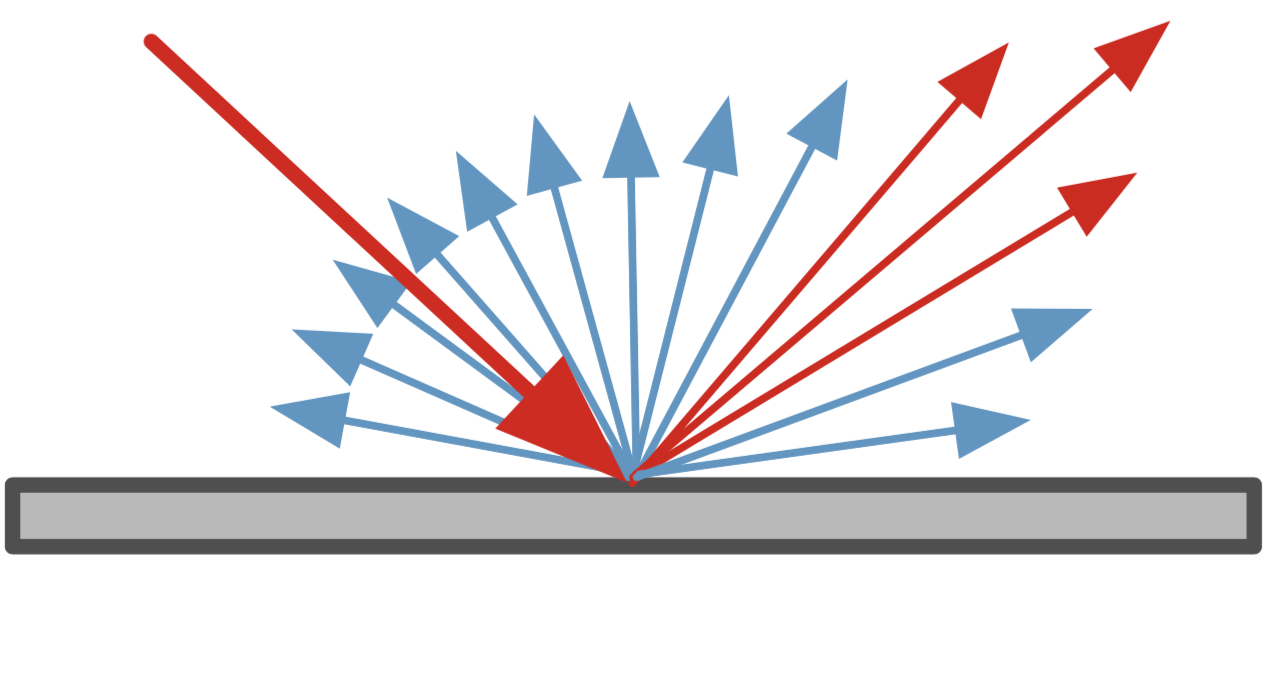
\includegraphics[width=\textwidth]{figures/vct/vct-1-1}
		\caption{光线追踪:大量光线}
	\end{subfigure}
	\begin{subfigure}[b]{0.5\textwidth}
		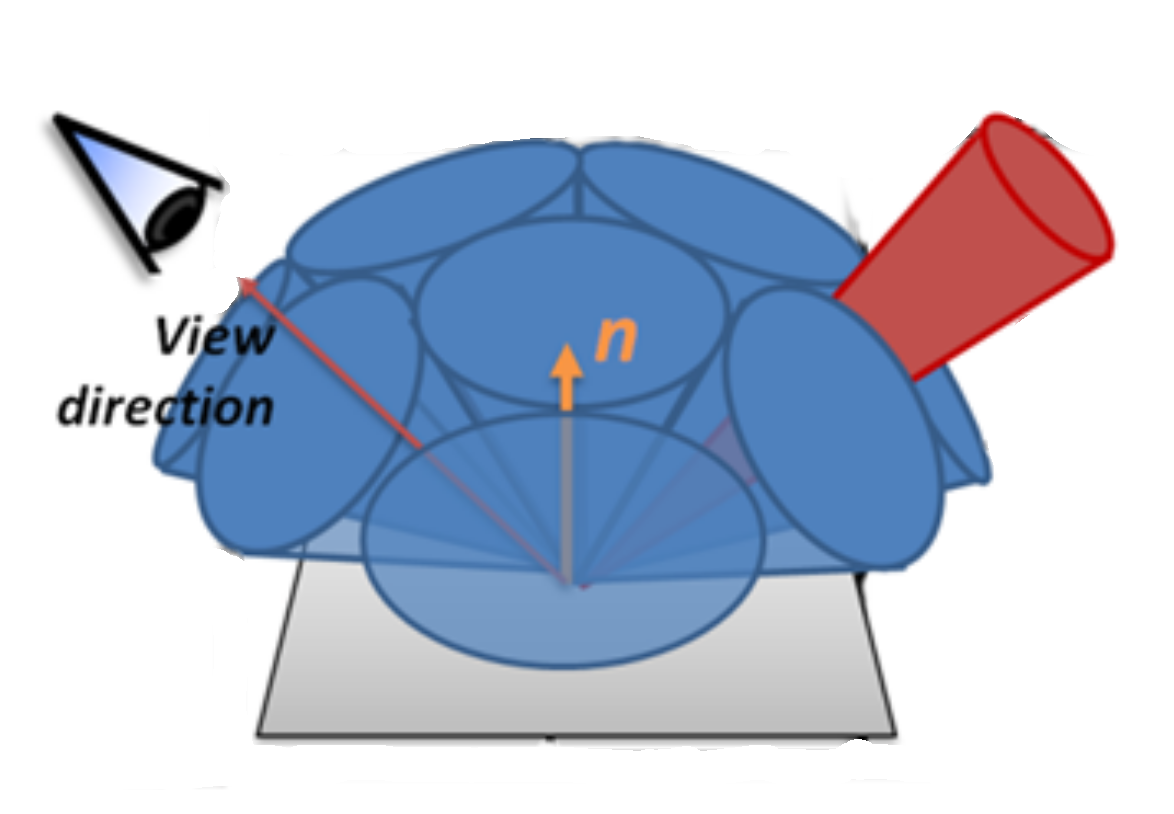
\includegraphics[width=\textwidth]{figures/vct/vct-1-2}
		\caption{圆锥体追踪:少量较大的圆锥体}
	\end{subfigure}
	\caption{光线追踪与圆锥体追踪的比较,在光线追踪中(a),当光线遇到与物体表面的一个交点时停止追踪,而在圆锥体追踪中 (b),沿圆锥方向上所有相交面积中的值被累积起来,大量的光线方向可以被单个圆锥体内的方向集合近似,这大大减少了光线“追踪”的计算量}
	\label{f:vct-ray-vs-cone}
\end{figure}

上述关于光线的定义的主要问题在于,每个像素对应相关的所有光线没有 保留足够的信息去执行反走样(anti-aliasing),每条光线仅仅允许我们在一个像素的面积范围内采样得到一个位置,但是它不知道关于这个采样点周围相邻的任意位置的信息,例如这些位置是否可见,在多大面积内采样是足够等。

在标准的光线追踪中,其唯一能够实现反走样的方法是使用更高的分辨率 进行采样,例如\cite{a:ray-tracing}提出了适应性超采样。但是,这种超采样技术 存在一些问题,首先是那些方差较大的像素对应的光线数量会急剧地增长;其次,一些较小的细节可能被这些样本所忽略。

一种能够应对上述采样问题的方法是修改上述关于“光线”的定义为一个 “圆锥体”,如图\ref{f:vct-ray-vs-cone}(b) 所示,此时一个“像素”表述的是屏幕上的一个“面积”而不是一个“点”,这种扩展的“光线”(即圆锥体)与物体的相交计算不仅能够决定该光线与某物体的相交测试是否发生,并且还能决定该“光线”的多少部分与该物体相交。这种部分覆盖信息足够针对面积执行简单的反走样,同时,一个像素内的任意细节都不会被忽略。



\subsection{工作原理}
那么,圆锥体追踪到底是怎么工作的呢?对于光线追踪和圆锥体追踪两种 技术,我们都尝试从一个点得到一定数量的关于入射辐射亮度的样本,这通过发 射某种形式的基元(例如光线追踪中的直线或者圆锥体追踪中的体积或面积),然后让这些基元与场景相交来进行计算,如图\ref{f:vct-2-1}所示。

\begin{figure}
\begin{center}
	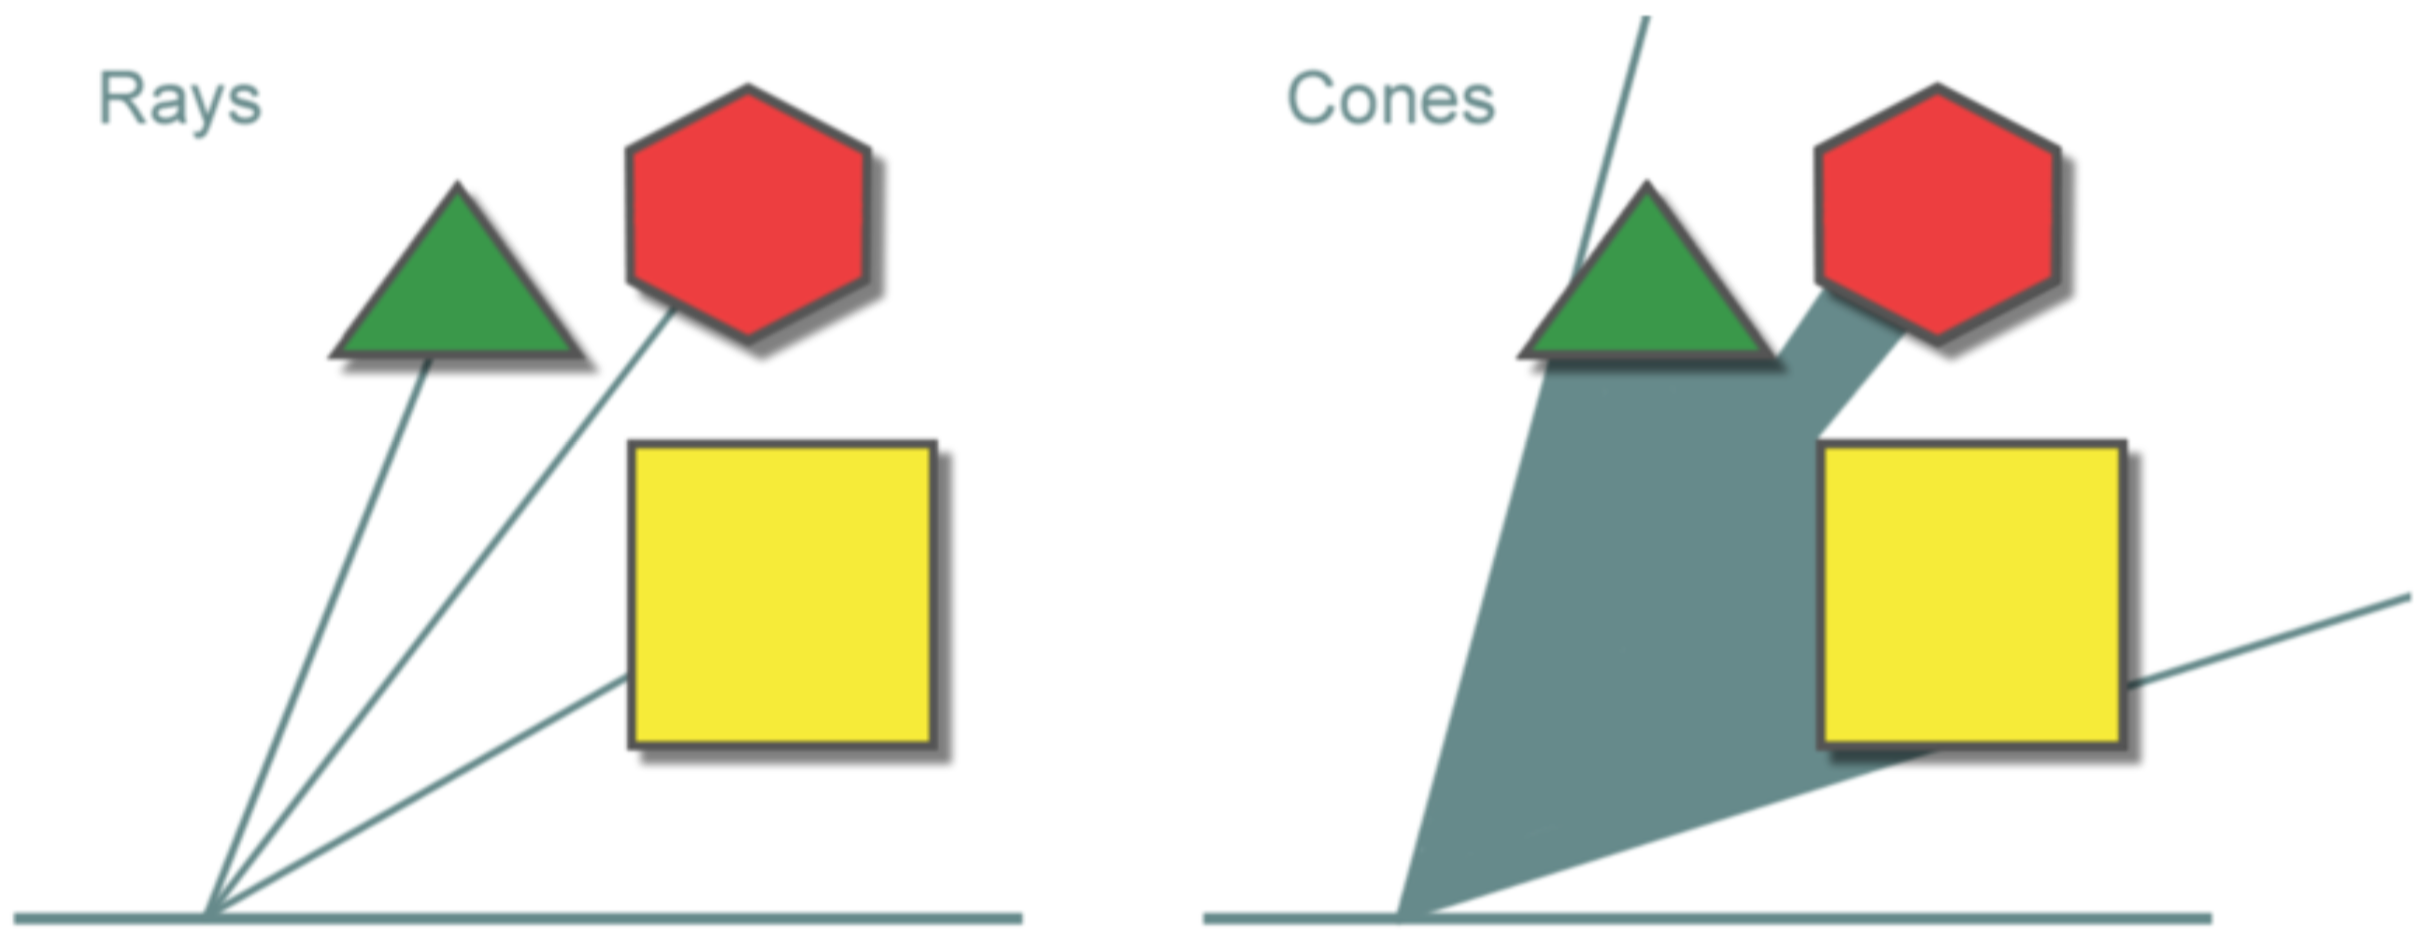
\includegraphics[width=0.8\textwidth]{figures/vct/vct-2-1}
	\end{center}
	\caption{在光线追踪中,光线与物体的相交发生于物体表面的一个点上(左图),而在圆锥体追踪中,相交的结果是一个面积或者一个体积,这取决于怎样看待相交部分(图片来自\cite{a:TheTechnologyofTheTomorrowChildren})}
	\label{f:vct-2-1}
\end{figure}

如果我们的得到足够多分布良好的光线样本,这些样本可以组合起来形成 对一个点处入射光照的一个估计,这些入射光照样本然后被与表面上该点处材质属性中的BRDF分布函数相作用,以计算该点处的出射光照。

所以,光线追踪与圆锥体追踪的主要区别在于,当我们计算各自表述光线 的基元与场景中的表面进行相交时发生了什么。在光线追踪中,光线线段与场景相交于一个点;而在圆锥体追踪中,其圆锥体与物体表面相交的结果是一个面积或一个体积,这取决于怎样看待相交的部分,如图\ref{f:vct-2-1}所示。

最重要的是,由于相交结果不再是一个无限小的点,光照估计的属性发生 了变化。首先,我们不再仅仅是寻找光线与物体表面一个位置处的交点,而是与圆锥体体积相交的物体表面的多个部分的交点;其次,由于需要计算一个相交的面积,因此场景必须是可过滤的,即我们得到的光照结果是一个平均值,因此其光照计算的精度会下降,但是另一方面,由于我们计算的是一个平均值,因此原本光线追踪容易产生的噪点被大大的消除了,因为对面积的积分(或者说 平均值计算)本质上就是一种过滤的思想。通过对体积(而不是单个点)的采样,从而使着色积分方程可以直接使用预过滤的结果,这是本章讲述基于体素全局光照技术的核心思路,因为这些预过滤的结果不仅可以区分不同的细节层次,还能够被重用以提高实时计算的效率。



\subsection{怎样采样}
尽管圆锥体追踪拥有上一节讨论的优点,但是它的相交计算却变得非常复 杂。考虑一个物体A,它的表面只有一部分与圆锥体相交,为了正确地渲染位于A后面的物体,新的光线定义(即圆锥体)必须能够指示位于A后面的物体有多少部分被A所遮挡。

这里的挑战是,怎样通过圆锥体(而不是光线)来进行采样,图\ref{f:vct-2-2}左小图中的紫色部分表示光线与物体表面相交的部分,这看起来并没有一种简单的方法能够计算出任意物体的相交部分,而在原来(即光线追踪)的直线定义中,这只要确定光线与物体是否相交即可,因为在那里只需要得到一个位置(点)采样,而不是一个表面上的任意面积。

\begin{figure}
\begin{center}
	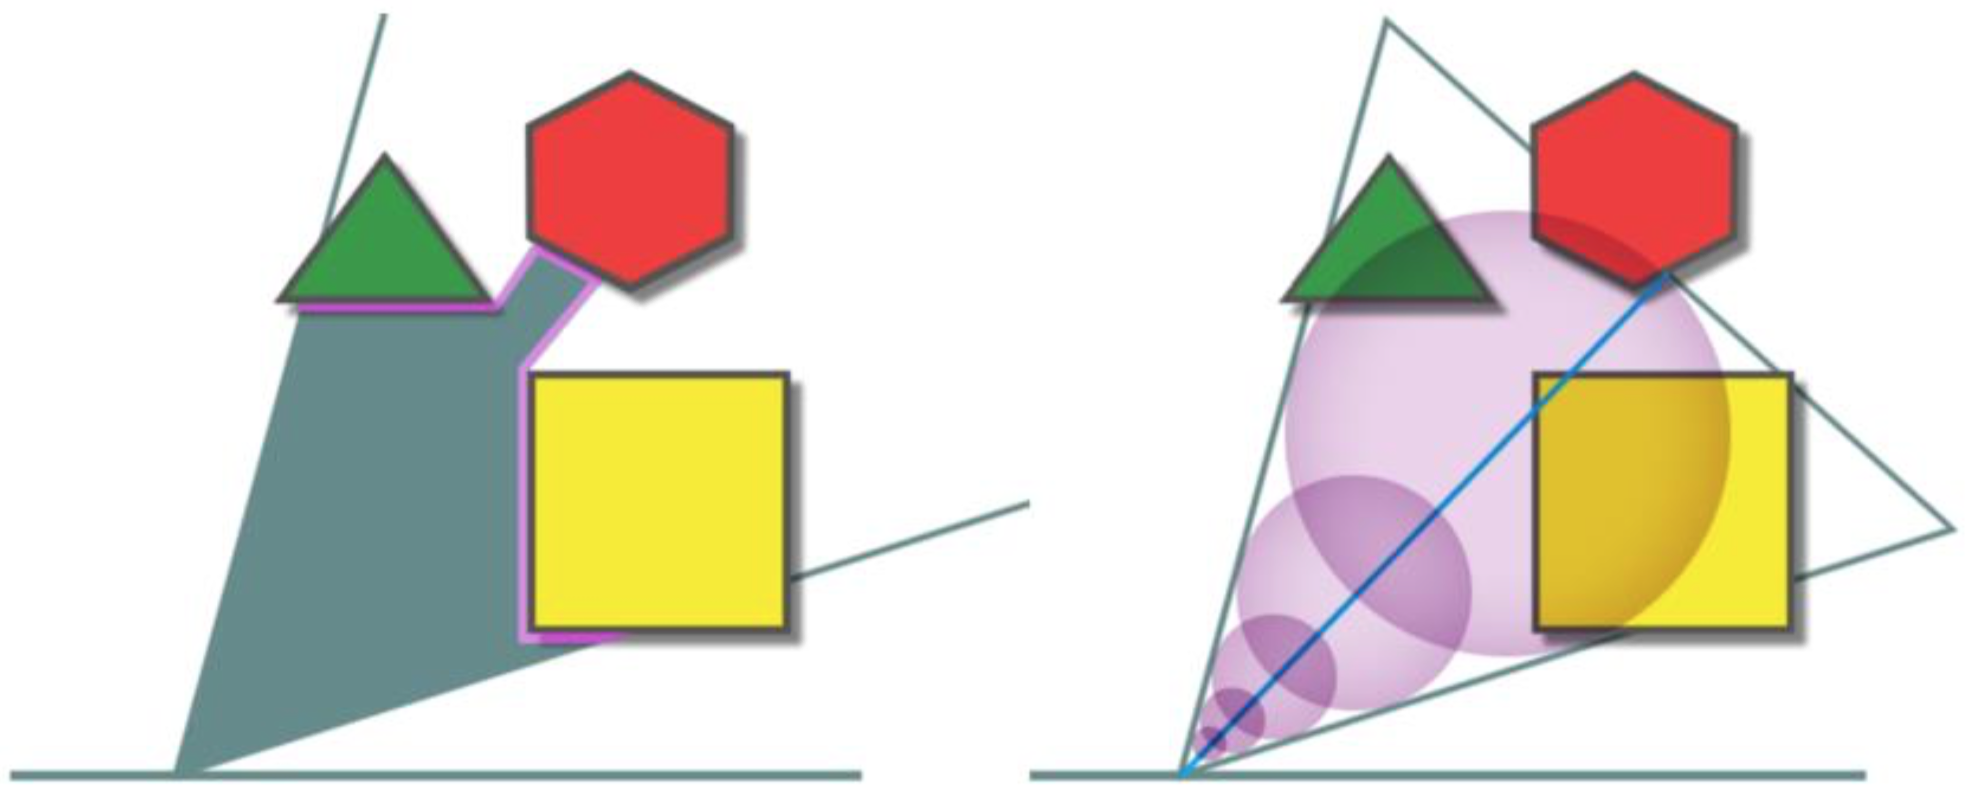
\includegraphics[width=0.8\textwidth]{figures/vct/vct-2-2}
	\end{center}
	\caption{圆锥体追踪对一个体积样本而不是一个点样本进行采样,它累积沿着圆锥体步进的每一个体积样本的贡献,每个体积样本既要返回该部分体积对圆锥体顶点的光照贡献,还要记 录该体积与圆锥体相交部分占据圆锥体截面的比例,即可见性(图片来自\cite{a:TheTechnologyofTheTomorrowChildren})}
	\label{f:vct-2-2}
\end{figure}

显然并没有一种简单而高效的方法能够计算如图\ref{f:vct-2-2}左小图中那种圆锥体与 表面相交的任意表面面积,因此,圆锥体追踪使用了一种近似方法,这种方法的思路来源于光线在参与介质中的步进,在光线的步进过程中,每个选择的位置会发射出光照,同时光线还会接受来自该样本位置后面的光线上样本的光照,这取决于该样本位置处的透射比。我们将会在第\ref{sec:vct-volumetric-presentation}推导这种基于体积渲染积分的采样方法。

所以相较于光线追踪,圆锥体追踪的相交测试需要计算出两个东西:一是 圆锥体是否与某个物体的某个部分相交,这涉及物体与物体之间的相交测试(而不是光线追踪中光线与物体的相交测试);二是每个物体相交部分所占圆锥体截面的比例,这相当于参与介质中的透射比系数。

为了避免求解与物体相交面的真实面积,我们提出一种称为体积样本(volume samples)\myindex{体积样本}{volume samples}的概念,如\ref{f:vct-2-2}右图中的紫色球体,每个体积样本返回两个值: 即该体积对圆锥体顶点处的光照估计,以及该体积对圆锥体遮挡的比例。有了这两个数据,我们可以按照参与介质中的光线步进的方式计算出圆锥体追踪过程中的光照值,即对这些相交物体进行由近到远的排序,然后对每个物体的光照贡献进行累加,而每个物体对圆锥体没有被遮挡的面积比例充当了透射比。



\subsection{精确度问题}
需要注意的是,由于我们使用了体积样本,当圆锥体被部分遮挡时,这可 能会得到不正确的结果,因为我们并没有记录遮挡物体的形状和位置信息,所以无法准确计算它对后面的体积样本的影响。

例如在图\ref{f:vct-2-3}的例子中,这里包含两个部分遮挡的物体,它们各自都遮挡 了 50\% 的光照,在实际情况下,在顶点处观察光照会被全部(即 100\%)遮挡。 然后在上一节讨论的圆锥体追踪的框架下,顶点处仍然能够观察到 25\% 的光照 没有被遮挡,因为这些与圆锥体相交的物体对顶点的光照贡献类似于透明度混合(alpha blending)\myindex{透明度混合}{alpha blending}的原理,即 25\% = 50\% * 50\%。

\begin{figure}
\sidecaption
	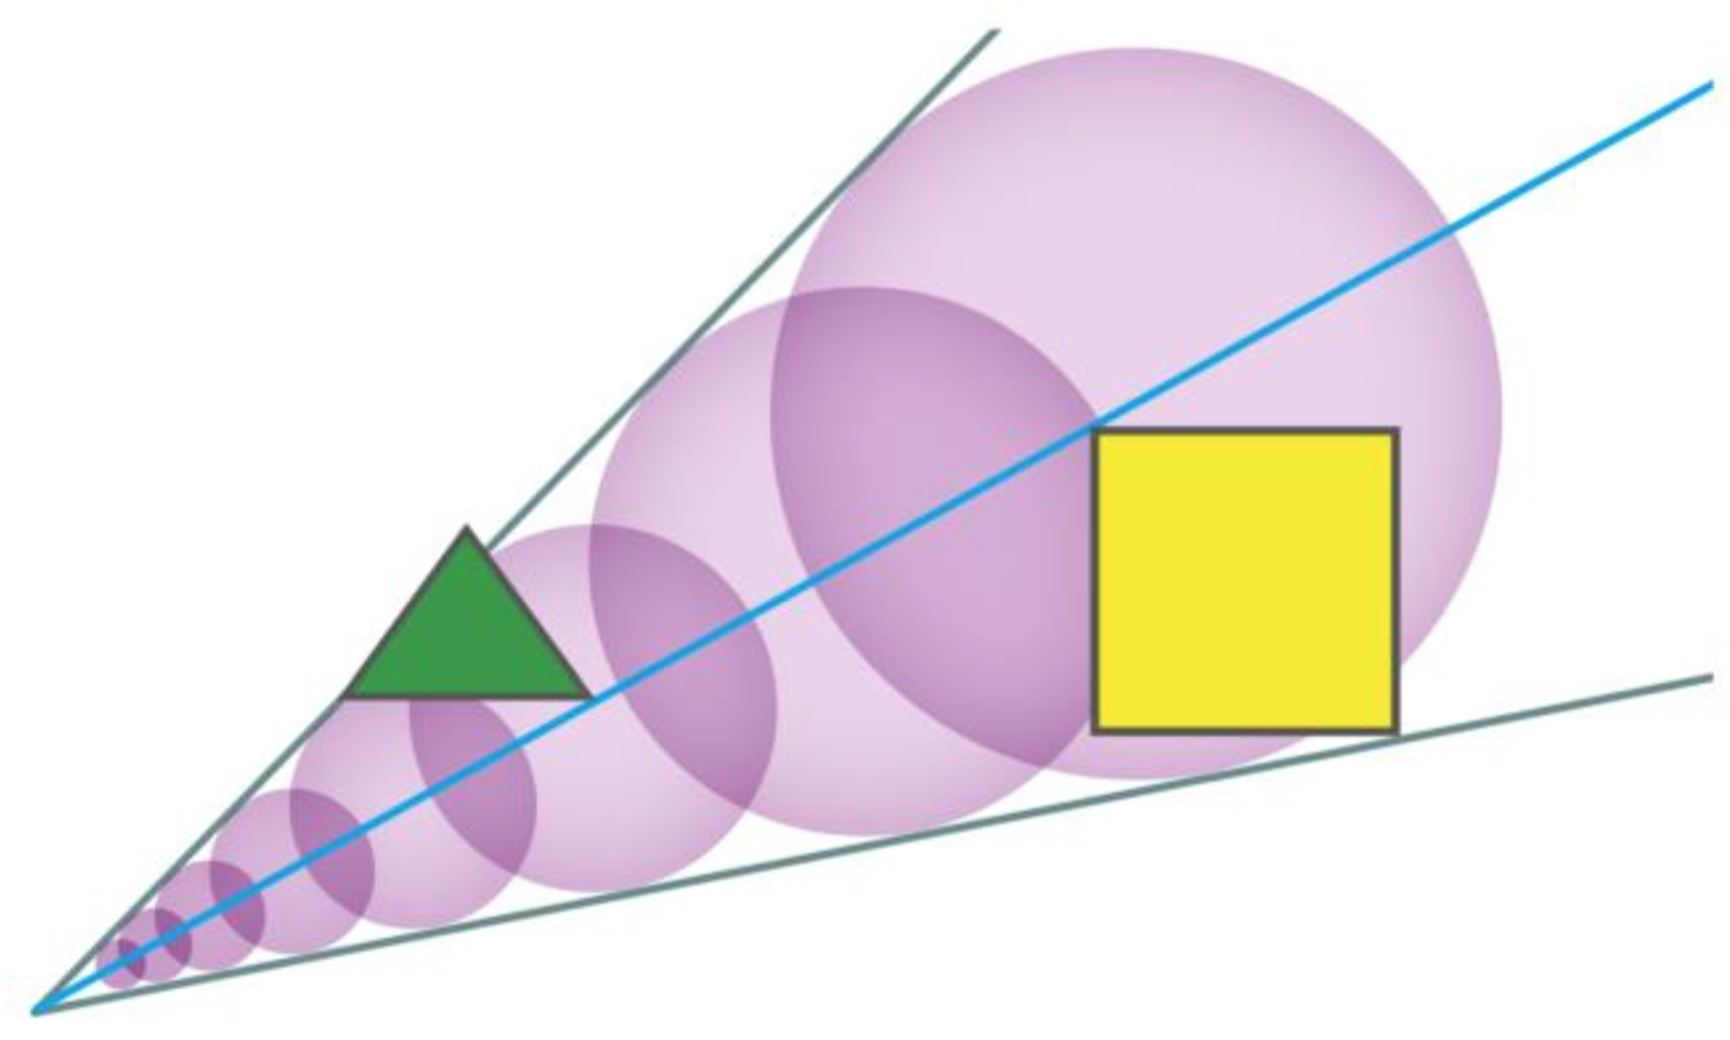
\includegraphics[width=0.55\textwidth]{figures/vct/vct-2-3}
	\caption{一个圆锥体被两 个物体遮挡,分别遮挡住50\%的空间,这本来应该使得圆锥体顶点处的光照完全被遮挡,但是由于圆锥体追踪采样了透明度混合的方式,因此却错误地得到 50\%∗50\% = 25\% 的光照(图片来自\cite{a:TheTechnologyofTheTomorrowChildren})}
	\label{f:vct-2-3}
\end{figure}

不过上述问题在实践中并不是一个很大的问题,但是我们需要明白的是圆 锥体追踪只是一个非常粗略的近似估计。




\section{体积化的几何表述}\label{sec:vct-volumetric-presentation}
很明显,通过使用圆锥体追踪,我们可以加速本章开头介绍的全局光照的 两个难题:即可见性和沿多个方向的积分计算。但是由于圆锥体追踪使用的是体积(而不是光线追踪使用的点)样本,所以我们还需要为传统的基于使用网格数据,以多边形表面的基元形式表述的场景找到一种新的的几何数据结构,即一种新的(不同于表面的)几何基元,使其可以和圆锥体追踪一起协同工作。

那么我们到底需要的是什么呢?从上一节的内容可以知道,圆锥体追踪的 过程就是累积所有沿着圆锥体步进位置处的光照信息(例如辐射照度),对一个面积(而不是单个点)的累积计算意味着我们需要对步进中的每一个面积执行预过滤(pre-filtering)\myindex{预过滤}{pre-filtering},所以我们需要的实际上就是对整个场景执行预过滤后的某种表述,这样在每一个步进中,我们可以直接得到这个预过滤的结果,即这个面积内某种量的平均值,如图\ref{f:vct-2-4}所示。

\begin{figure}
\sidecaption
	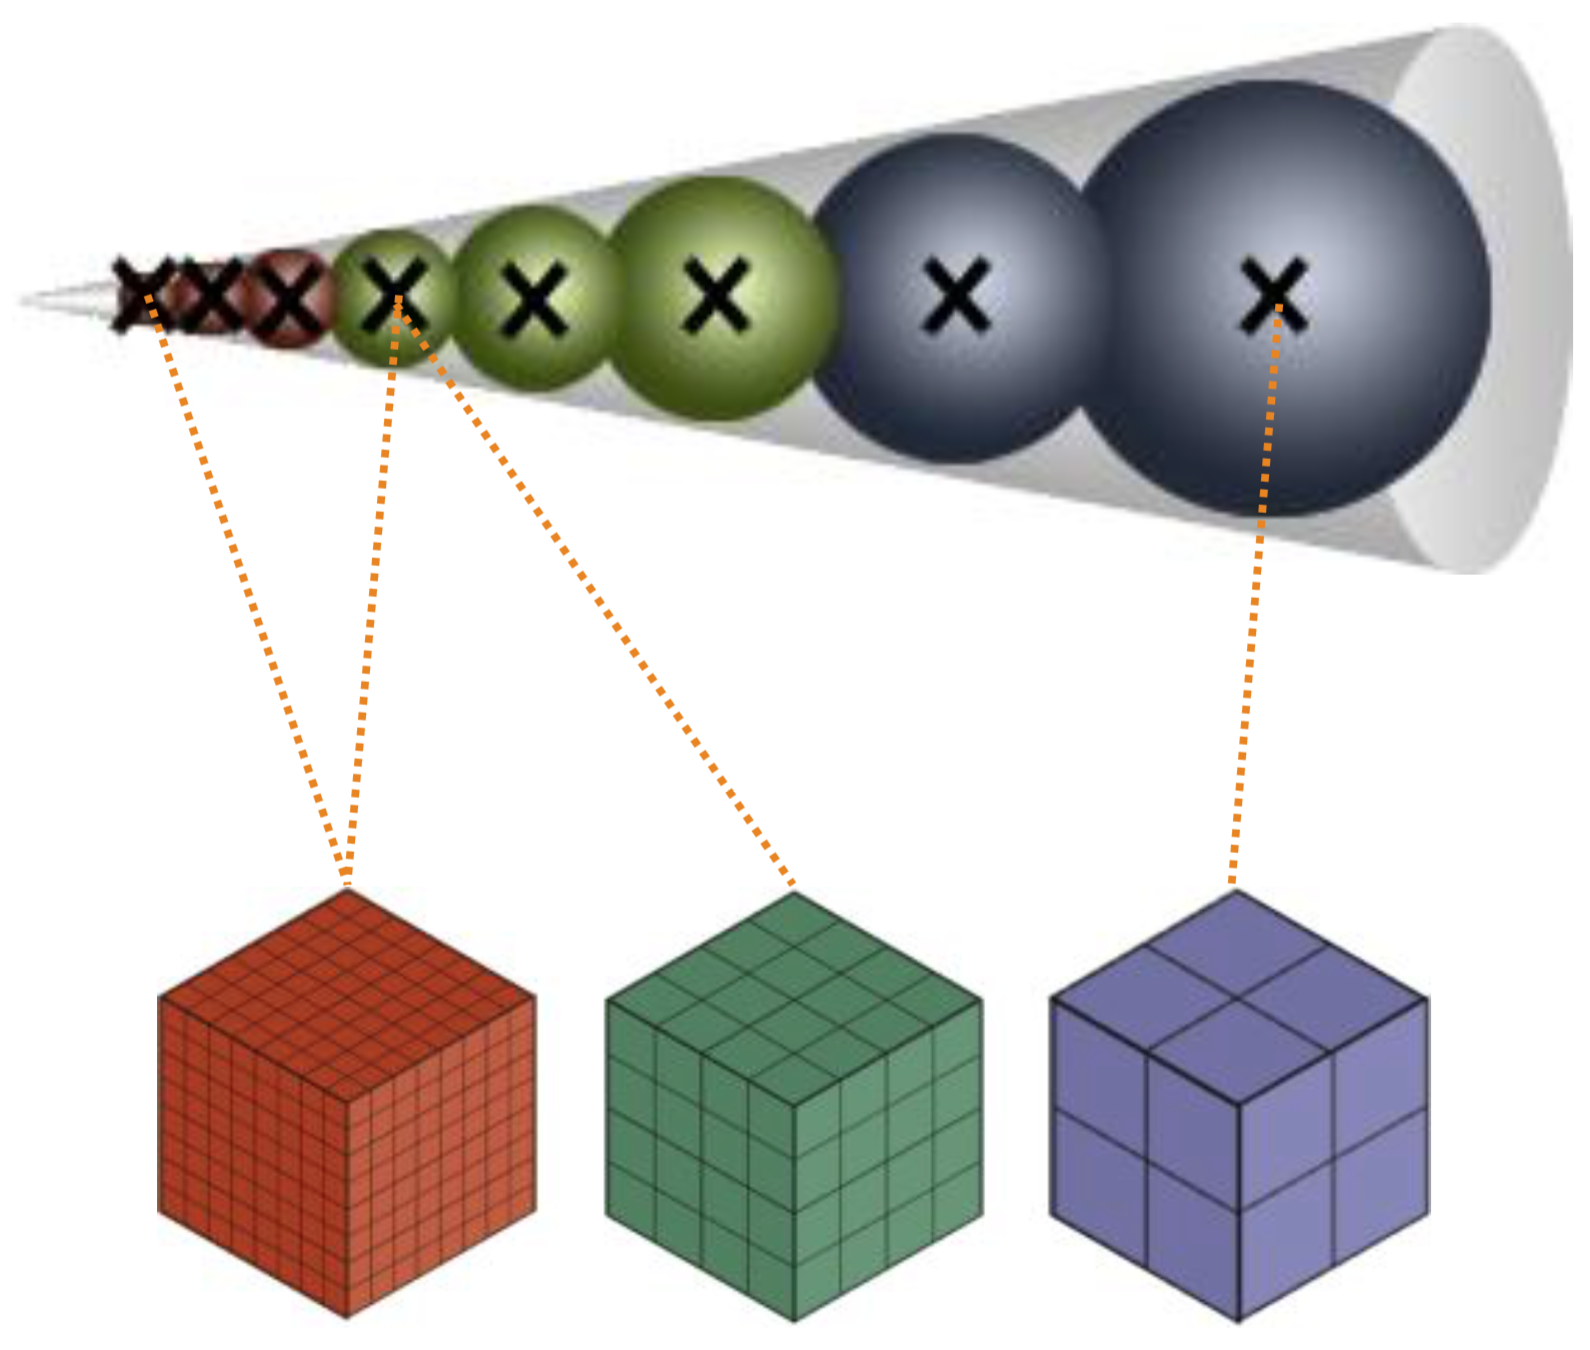
\includegraphics[width=0.5\textwidth]{figures/vct/vct-2-4}
	\caption{在圆锥体追踪的每一次步进中,它直接从一个预过滤的几何表述中获取一个预过滤的某种量的值来计算顶点处的光照}
	\label{f:vct-2-4}
\end{figure}

这就是本章基于体素的全局光照技术的核心思路,在这种算法中,我们使 用一个体素八叉树来表述整个场景,然后将每个体素对应体积内的辐射亮度预过滤到整个八叉树结构中,这样后续圆锥体追踪就可以直接从这个八叉树中获 取阴影遮挡和间接光照值。

在本节,我们将详细表述这种阶层式的体素结构,例如怎样选择特定的数 据结构,怎样对体素内的值执行预过滤,以及体素内的各种数据(例如遮挡和辐射亮度等)被怎样表述。



\subsection{基于体素的几何预过滤}
由前面的定义可知,我们需要的是一个对网格场景执行预过滤的几何表述,这样我们便可以使用圆锥体追踪来加速光照传输的计算。

基于线性的假设,预过滤的核心思路是,当计算围绕一个面积(例如一个 像素)的积分的时候,我们可以将着色方程中的一些参数提取出来,并对这些参数围绕该面积的积分单独预计算出来,这也称为预积分\footnote{在本章,我们需要仔细区分预过滤和预积分的概念,预积分是指提前计算任意一个积分在 任意一些位置处的值,所以预过滤是一种特殊形式的预积分,预过滤则通常是指被积函数中 含有一个加权和为 1 的核函数,这形成一种线性关系,这样我们可以根据这个核函数对被积 函数在各个分辨率进行预过滤,而预积分的值则不能被这样“统一”计算,它需要单独计算每 个位置处的积分值。本章后面我们将看到怎样从一个预积分中提取出线性部分,并使这部分 转换为一个预过滤结果的形式。}(pre-integrating)\myindex{预积分}{pre-integrating}, 或者预平均(pre-averaging)\myindex{预平均}{pre-averaging}。这个操作使我们可以移除一个像素范围内高于渲染分辨率的频率,同时保留像素内相应参数的平均值。这种几何预过滤提供一种只与渲染分辨率相关的可伸缩性,使得可以处理非常复杂的场景。

对几何体执行预过滤的思考主要来源于\cite{a:hypetrtexture}和\cite{a:Renderingfurwiththreedimensionaltextures} ,考虑一个包含许多随机分布的表面的体积,例如图\ref{f:vct-4-1}左小图中体积内的树枝和叶子,当计算光与该体积内物体的综合\footnote{这里的综合指英文单词overall,指大体上的或者平均而言,因为该体积已经是一个最小的单位,我们无法更精确地处理该单位内的细节。这有点类似于使用一个综合的 BRDF 分布函 数来近似一个像素内微观面元的法线分布。}光照交互时,体积 内那些表面的准确位置和法线分布信息并不重要。因此,我们可以使用一个综合密度分布函数(overall density distribution function)\myindex{综合密度分布函数}{overall density distribution function}和一个综合反射函数来 近似光与这个体积(内所有表面)的交互,如图\ref{f:vct-4-1}右小图所示。

\begin{figure}
\sidecaption
	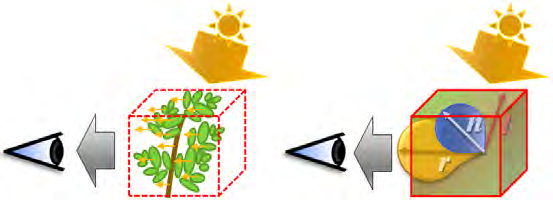
\includegraphics[width=0.65\textwidth]{figures/vct/vct-4-1}
	\caption{对一个体素元素内 复杂几何细节的预过滤示意 图,这使得我们可以从预过滤的结果中计算一个综合的(overall)着色光照贡献(图片来自\cite{a:InteractiveIndirectIlluminationUsingVoxelConeTracing})}
	\label{f:vct-4-1}
\end{figure}


所以,当考虑一个体积内部的这些复杂的表面的定义的时候,相较于原始 的基于网格的表面定义,将那些用于着色计算的参数表述为体积的形式是一种更好的选择。在这种体积表述下,那些描述体积内的各个细节表面与光进行交互的着色参数被表述为一个(体积内的)密度分布函数,而不是像原来的方式 直接定义在表面上。换句话说,我们将场景的表面参数化转化为了一种体积的 形式,体积成了一种渲染所需要的基元(primitive)类型,而体积内的分布函数就是对这种基元类型的参数化。一旦场景中的几何物体被转化为这种密度分布,对这些分布函数执行过滤(积分)就变成一种简单的线性操作。

体素(voxel)\myindex{体素}{voxel}这个词是体积像素(volumetric pixel)\myindex{体积像素}{volumetric pixel}的缩写,它是 2D 平 面上的像素的概念在 3D 空间中的一般化。体素是存储 3D 体积数据的一般方 法,它们被组织为沿着坐标轴均匀细分的网格,如图\ref{f:vct-4-2}所示。体素表述提供 了一种很好的统一纹理和几何表述同时又简化过滤的方法,它具有很强的表述 能力,并且其规则化的结构也非常利于对体素进行操作,例如添加或删除一些 体素数据,这些因素使得原本在传统的三角化模型中非常难于处理的反走样问 题变得非常简单。

\begin{figure}
\sidecaption
	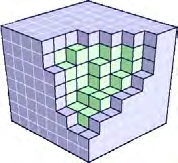
\includegraphics[width=0.3\textwidth]{figures/vct/vct-4-2}
	\caption{体素的示意图,它 是像素的概念在 3D 空间的 一般化(图片来自\cite{a:InteractiveIndirectIlluminationUsingVoxelConeTracing})}
	\label{f:vct-4-2}
\end{figure}

体素也可以采样类似多级纹理的思路来表述体积内分布函数的的多种分辨 率,这使得外部可以根据细节层次选择对应的结果。在图\ref{f:vct-4-3}中,通过在层级 之间进行插值计算,多级体素可以使得渲染被使用的几何分辨率能够很好地匹配屏幕分辨率,由于体素表述的已经是预过滤的数据,因此这种基于体素的采 样可以实现和超采样相似的反走样能力和效果。

\begin{figure}
	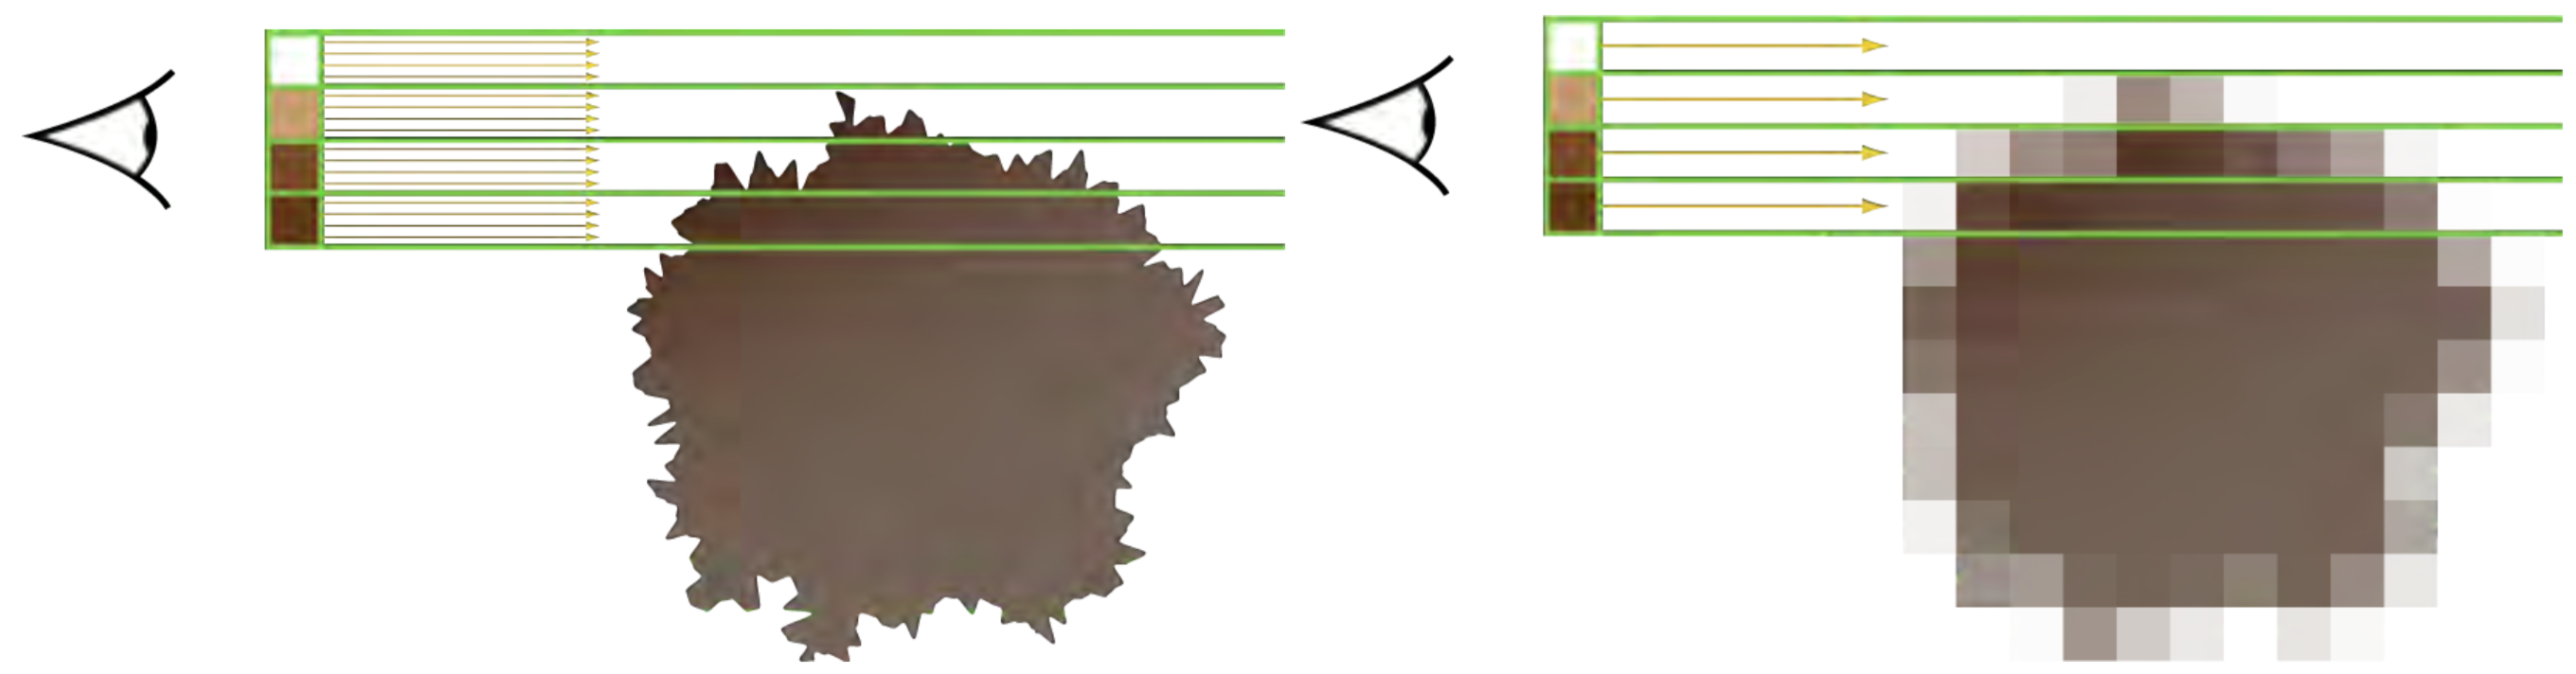
\includegraphics[width=\textwidth]{figures/vct/vct-4-3}
	\caption{左图描述了一个包含非常多细节的物体通过 4 个像素采样超采样进行渲染,右图使 用基于体素的预过滤技术,每个体素包含了该体素内部表面细节的平均值,这些预过滤的均 值使得采样需要的样本数量大大减少,提高了渲染效率(图片来自\cite{a:InteractiveIndirectIlluminationUsingVoxelConeTracing})}
	\label{f:vct-4-3}
\end{figure}



\subsection{基于预积分的圆锥体追踪}\label{sec:vct-pre-integration-based-cone-tracing}
有了关于圆锥体追踪和几何体体素表述的概念,本节我们将推导出基于对 体素预积分的圆锥体追踪渲染算法框架。

在传统的基于边界的表面表述中,各个物体之间并不能被线性组合起来, 对这种表面的预过滤只发生与单个物体内部,即对每个物体自身的纹理执行预 过滤得到该物体的一个多级纹理,这种情况下着色计算只能在物体内部选择相 应的细节层次,而不能在表面之间进行组合。然而在基于体素的表述中,所有 参数都被转化为了一个统计的密度分布并存储在规则的体素中,因此体素内的 所有表面参数都可以被线性的预过滤并存储在一个体素多级金字塔结构中。

在本节的上下文中,我们希望在多个分辨率级别存储预过滤的材质和几何信息,这样便可以高效的渲染非常复杂的场景,并且能够动态地计算所有分辨 率下的光照交互。一般来说,我们至少需要对每个体素存储一个过滤的透明度, 材质颜色以及法线分布等信息(这些数值的计算将在下一节讨论)。

自从第一次在\cite{a:Thealiasingproblemincomputer-generatedshadedimages}中被讨论,走样已经成为渲染中的一个主要问题。由于屏幕上的一个像素并不仅仅对应空间中的一条直线,实际上每个像素对应着一个圆锥体,因为每个像素并不是一个点,而是覆盖着一定的面积,因此当由摄像机向像素发出光线时,这些光线坐落于由摄像机作为顶点,像素的扩展面积构成的圆锥体内,如图\ref{f:vct-6-1}所示。这就是当单个光线被用于对场景采 样时走样始终会发生的原因。

\begin{figure}
\sidecaption
	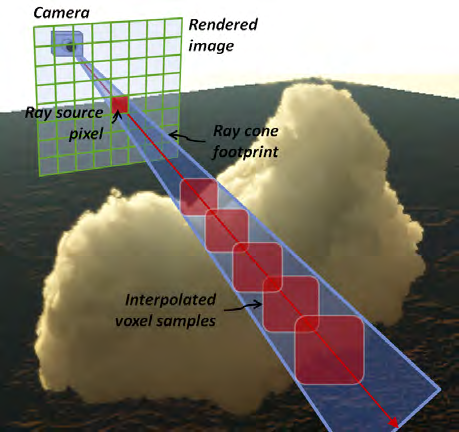
\includegraphics[width=0.55\textwidth]{figures/vct/vct-6-1}
	\caption{光线由摄像机发 出,经过有一定面积的像 素,构成一个类似圆锥体形 状的光束,这个光束的光照 可以使用这样的方式进行近 似计算:即一个单束的光线 由像素位置处发出,然后对 一个预过滤的体积表述进行 采样(图片来自\cite{a:InteractiveIndirectIlluminationUsingVoxelConeTracing})}
	\label{f:vct-6-1}
\end{figure}

为了计算来自圆锥体足迹内入射辐射亮度的积分,我们需要对圆锥体内的 所有位置$D$ 处入射方向$\omega$上的入射辐射亮度$I(D,\omega)$ 执行进行积分,即:

\begin{equation}
	I=\int_{\Omega}I(D,\omega){\rm d}\omega
\end{equation}

在传统的超采样方法中,该积分被离散化为多条(通常远高于屏幕分辨率 的)光线以克服走样的问题,这导致巨大的计算成本。另外的一些方法,如原始的圆锥体追踪和光束追踪(beam tracing),它们依赖于对几何场景的解析表述,这种方法不利于处理一般化的几何复杂度。在本节,我们将提出一种基于每像素只发射单个光线的模型,它可以通过使用来自于多级体素金字塔结构中预过滤的几何表述来处理走样的问题。

上述近似的圆锥体追踪基于一个假设,即我们可以使用一个预积分的可见 性值来近似一个圆锥体内的可见性(这将在后面的内容中看到)。这种模型基于经典的体积渲染积分模型,我们将在下一节一步一步详细推导这个基于预积分的渲染模型,并且会说明该模型推导过程中使用的一些近似假设。




\subsubsection{体积渲染}
尽管本书前面已经介绍过体积积分,但为了保证知识的连贯性,本节还是 首先对其进行简要的回顾,同时这里也会说明一些针对本节相关的内容。

在体积渲染(volume rendering)\myindex{体积渲染}{volume rendering}中,沿着一条穿过一个参与介质的光线的辐射亮度受三种不同类型交互的影响:即发射,吸收和散射,其中发射(emission)\myindex{发射}{emission}是指参与介质内部各个位置处直接发射出的辐射能量,吸收(absorption)\myindex{吸收}{absorption}是指 在参与介质内部传输时被吸收的辐射能量,散射(scattering)\myindex{散射}{scattering}是指参与介质散 射来自外部(非自发射)的辐射能量,散射的结果使得光的传播方向被改变,由此可以看出,散射可以增加(如向内散射)或减少(向外散射)沿一个方向传 播的辐射能量,如图\ref{f:pm-medium-properties}所示。

考虑一个沿着一个直线段上的量$s$,表述为 $x = p + s\omega$,$p$ 为一个任意的参考位置,其光照传输的方程为:

\begin{equation}
	\cfrac{{\rm d}I(s)}{{\rm d}s}=-\chi(s)I(s)+\eta(s)
\end{equation}

\noindent 其中, $\chi(s)$ 表示总的吸收系数,它定义为两个系数 $κ$ 和 $\sigma$ 的加和,其中前者表示吸收系数,而后者表示向外散射系数,即 $\chi = \kappa + \sigma$;$\eta(s)$ 表示总的发射系数,它是另外两个系数 $q$ 和 $j$ 的加和,其中前者表示发射系数,后者表示 向内散射系数,即 $j: \eta = q + j$。

在本节相关的内容中,我们将仅考虑发射和吸收,即忽略散射和其它间接光照,在这种模型下,光照传输模型可以简化为:

\begin{equation}
	\cfrac{{\rm d}I(s)}{{\rm d}s}=-\kappa(s)I(s)+q(s)
\end{equation}

上述的积分微分方程可以被转化为一个积分方程求解,该积分方程沿着光 线以从后向前的方向,在以起点为 $s = s_0$,终点为 $s = D$ 的区间内进行积 分计算。定义起点 $s = s_0$ 处的初始辐射亮的为 $I_0$,则体积渲染积分可以表述 为\cite{b:Real-timeVolumeGraphics}:

\begin{equation}
	I(D)=I_0 {\rm e}^{-\tau(s_0,D)}+\int^{D}_{s_0}q(s){\rm e}^{-\tau(s,D)}{\rm d}s
\end{equation}

\noindent 其中, $\tau(s_1,s_2)$ 称为位置 $s_1$ 和 $s_2$ 之间的光学深度(optical depth)\myindex{光学深度}{optical depth}或者光学厚度(optical thickness)\myindex{光学厚度}{optical thickness},它描述的是光线在部分透明的参与介质中传播的 吸收或散射比例,定义为:

\begin{equation}
	\tau(s_1,s_2)=\int^{s_2}_{s_1}\kappa(t){\rm d}t
\end{equation}

\noindent 定义透明度为 T (s1, s2) ∈ [0, 1]:

\begin{equation}
	T(s_1,s_2)={\rm e}^{-\tau(s_1,s_2)}
\end{equation}

\noindent 则体积渲染积分可以简化为:

\begin{equation}
	I(D)=I_0T(s_0,D)+\int^{D}_{s_0}q(s)T(s,D){\rm d}s
\end{equation}




\subsubsection{体积积分理论}
在上述的模型中,我们考虑在光线 $r$ 上点 $s$ 处的总的吸收系数 $\chi (s, r)$,当 使用上述参与介质的来表述过滤的几何体时,该几何表述几乎不会从自身发射 光照,它仅仅会从其它外部光源反射光照,因此我们这里不再考虑自发光系数 $q$,而是考虑向内散射系数 $j(s, r)$,它表述的是在过滤的几何表面上在点 $s$ 处沿 光线 $r$ 散射的能量。

如图\ref{f:vct-7-1}所示,我们首先假设一个通过对像素足迹执行一个平行的投影产生的一个正交的光束,后面将会介绍怎样将这个正交模型扩展为根据圆锥体光 束形成的透视投影模型。

\begin{figure}
\begin{center}
	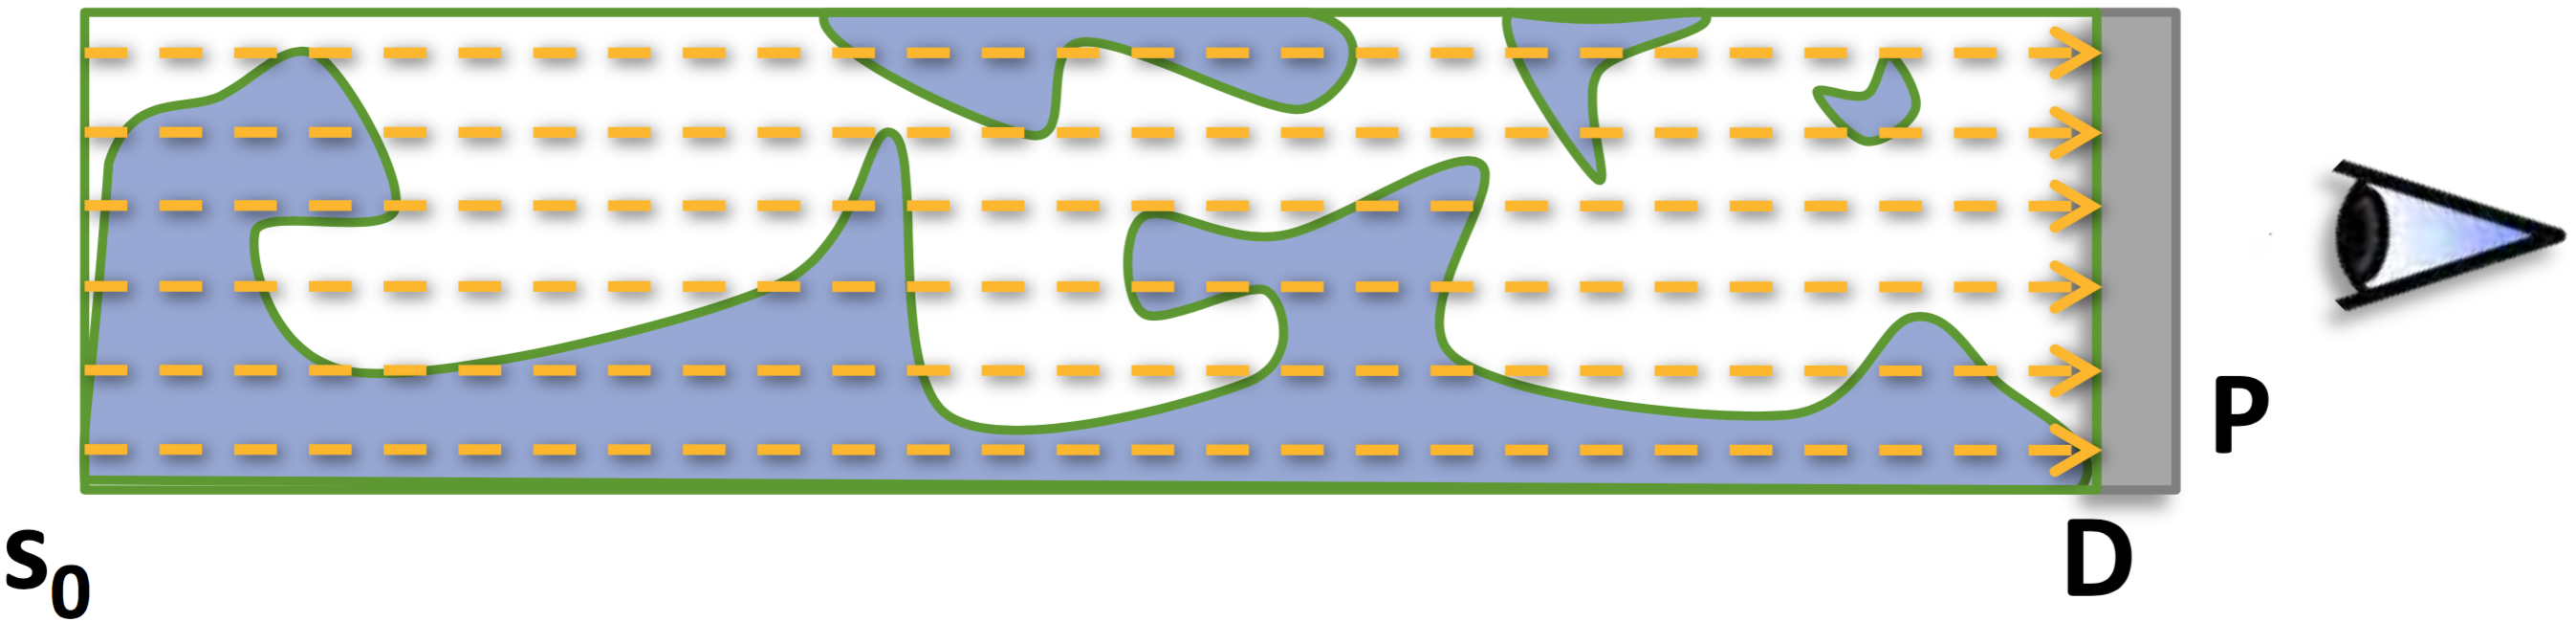
\includegraphics[width=0.8\textwidth]{figures/vct/vct-7-1}
	\end{center}
	\caption{以正交的方式,沿着一个像素足迹的体积渲染积分(图片来自\cite{a:InteractiveIndirectIlluminationUsingVoxelConeTracing})}
	\label{f:vct-7-1}
\end{figure}

我们的目标是建立一个预积分模型(pre-integration model)\myindex{预积分模型}{pre-integration model},该模型计算 沿着一个像素 $P$ 的足迹累积的平均能量 $I(D,P)$。这可以模型化为一个沿着光 线 $r$ 并围绕像素 $P$ 的足迹(即像素所占据的面积)的双重积分,即:

\begin{equation}\label{e:vct-double-integration}
	I(D,P)=\int_{r\in P}\int^{D}_{s_0}j(s,r){\rm e}^{-\int^{D}_s\chi (t,r){\rm d}t}{\rm d}s{\rm d}r
\end{equation}

对于上述的积分,这里提出的方法是将其替换为多个立方体体积内的预积分(pre-integration)\myindex{预积分}{pre-integration},如图\ref{f:vct-7-2}所示,我们的目标是存储在一个 3D 金字塔层 级结构中存储一些离散的这种预积分结果,使其能够被用来加速渲染的计算。

\begin{figure}
\begin{center}
	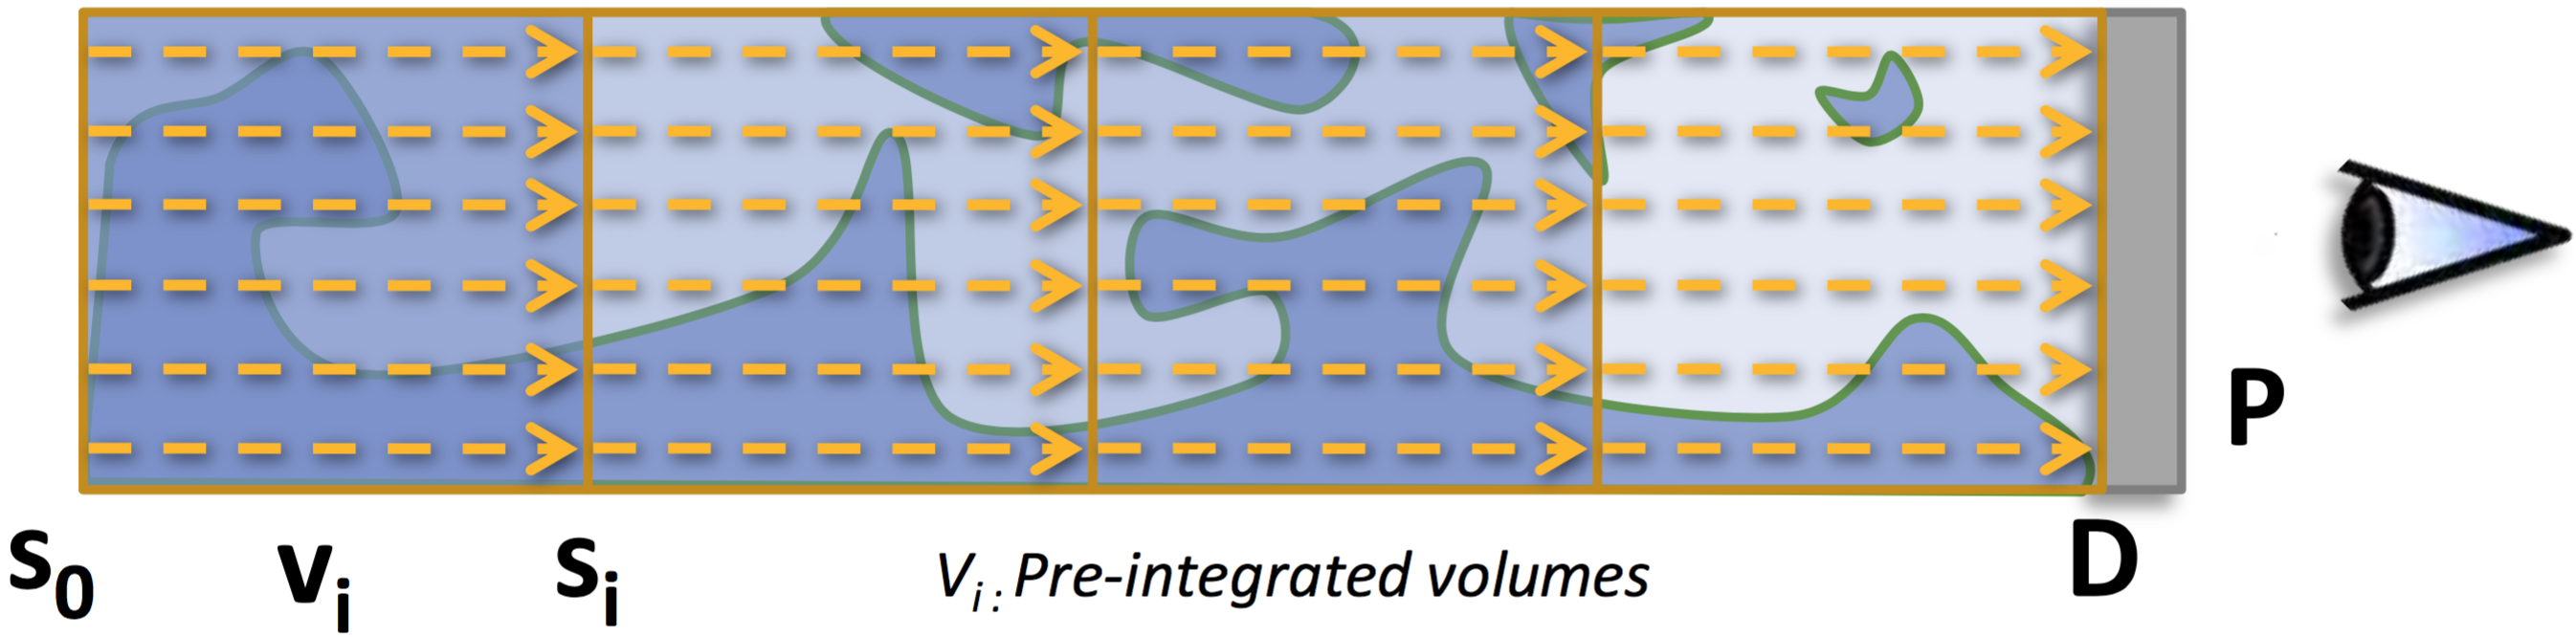
\includegraphics[width=0.8\textwidth]{figures/vct/vct-7-2}
	\end{center}
	\caption{原始完整的体积渲染积分,被转换为多个子体积内预计算的结果的累积(图片来自\cite{a:InteractiveIndirectIlluminationUsingVoxelConeTracing})}
	\label{f:vct-7-2}
\end{figure}

首先,我们需要将式\ref{e:vct-double-integration}中沿着单个光线的体积积分分拆为多个能够被预 计算的离散的子积分,为了简化方程的表述,这里定义 $\tau(s_1,s_2)$ $s_1$ 到 $s_2$ 之间沿着光线 $r$ 的光学深度,即:

\begin{equation}
	\tau(s_1,s_2,r)=\int^{s_2}_{s_1}\chi(s,r){\rm d}s
\end{equation}

\noindent 同时定义 $Q(s_1, s_2, r)$ 为 $s_1$ 到 $s_2$ 之间的向内散射能量:

\begin{equation}
	Q(s_1,s_2,r)=\int^{s_2}_{s_1}j(s,r){\rm e}^{-\tau (s,s_2,r)}{\rm d}s
\end{equation}

于上述的定义,原始基于区间 $[s_0, D]$ 上的积分可以被拆分为多个离散区间 $[s_i, s_{i+1}]$ 上的积分,即:

\begin{equation}
	I(D,P)=\int_{r\in P}\sum^{n}_{i=0}\bigg(Q(s_i,s_{i+1},r)\cdot {\rm e}^{-\sum^{n}_{j=i+1}\tau (s_j,s_{j+1},r)}\bigg){\rm d}r
\end{equation}

这些离散的加数项其实代表了传统光线追踪算法中沿光线的每一个步进(marching)过程。根据富比尼定理(Fubini’s theorem)\mathindex{富比尼定理}{Fubini’s theorem}\cite{m:Fubinitheorem},基于所有函数的连续性(所有这些参数在空间中都是连续的),我们可以在 整个表达式中将离散加和和积分进行交换,这得到以下的表达式:

\begin{equation}
	I(D,P)=\sum^{n}_{i=0}\bigg(\int_{r\in P} Q(s_i,s_{i+1},r)\cdot {\rm e}^{-\sum^{n}_{j=i+1}\tau (s_j,s_{j+1},r)}\bigg){\rm d}r
\end{equation}

现在需要一个的假设:对于给定的一条光线 $r$, 每段子区间内能量的积分 $Q(s_i,s_{i+1},r)$${\rm e}^{-\sum^{n}_{j=i+1}\tau(s_j,s_{j+1},r)}$ 之间是无关 的,后者表述的是 $s_{i+1}$ 到摄像机区间内的所有被吸收的能量的积分。这意味 着上述两项的值是统计无关的,基于这种假设,根据统计相关性的定义,即 ${\rm correlation}(a(), b()) = \int a()b() − \int a() \int b()$,可以将上述两个无关项乘积 的积分替换为它们积分的乘积,即:

\begin{equation}
	I(D,P)\approx \sum^{n}_{i=0}\Bigg( \bigg(\int_{r\in P} Q(s_i,s_{i+1},r){\rm d}r\bigg) \cdot \bigg(\int_{r\in P}{\rm e}^{-\sum^{n}_{j=i+1}\tau (s_j,s_{j+1},r)}{\rm d}r\bigg)\Bigg)
\end{equation}

由于有了这个假设,我们已经得到一个向内散射能量的公式,该公式以区间$s_1$ 到$s_2$ 内的预积分的形式存在,即:$\overline{Q}(s_1,s_2,P)=\int_{r\in P}Q(s_1,s_2,r){\rm d}r$ 。

现在使用类似的方法得到光学深度的预积分表达式,这需要将围绕 $P$ 的积分代入到指数项中光学深度加和的内部去。同样,这里首先将指数项汇总光学深度的加和提到外部形成一个指数的乘积的形式,即:

\begin{equation}
	I(D,P)\approx \sum^{n}_{i=0}\Bigg( \bigg(\int_{r\in P} Q(s_i,s_{i+1},r){\rm d}r\bigg) \cdot \bigg(\int_{r\in P}\prod^{n}_{j=i+1}  {\rm e}^{-\tau (s_j,s_{j+1},r)}{\rm d}r\bigg)\Bigg)
\end{equation}

上式正是传统的沿一条光线对离散点计算透明度的公式,即 $T(s_1,s_2,r) = {\rm e}^{−\tau(s_1,s_2,r)}$。有了这个公式,为了计算透明度的预积分, 唯一需要做的就是交换围绕 $P$ 的积分和乘积两个操作,同样基于前面相关性的假设,有:

\begin{equation}
	I(D,P)\approx \sum^{n}_{i=0}\Bigg( \bigg(\int_{r\in P} Q(s_i,s_{i+1},r){\rm d}r\bigg) \cdot \prod^{n}_{j=i+1}\bigg(\int_{r\in P}  {\rm e}^{-\tau (s_j,s_{j+1},r)}{\rm d}r\bigg)\Bigg)
\end{equation}

现在得到两个我们希望预计算并存储在体素表述中的函数,即平均向内散射能量$\overline{Q}$和平均透明度$\overline{T}$:

\begin{equation}\label{e:vct-pre-intergation-item}
	\begin{aligned}
		\overline{Q}(s_1,s_2,P)=&\int_{r\in P}Q(s_1,s_2,r){\rm d}r\\
		\overline{T}(s_1,s_2,P)=&\int_{r\in P}{\rm e}^{-\tau(s_1,s_2,r)}{\rm d}r
	\end{aligned}
\end{equation}

这样,我们便得到一个能够实时计算积分的方案,即:

\begin{equation}\label{e:vct-pre-intergation}
	I(D,P)\approx\sum^{n}_{i=0}\Biggl(\bigg(\overline{Q}(s_1,s_2,P)\Bigg)\cdot \prod^{n}_{j=i+1}\Biggl(\overline{T}(s_1,s_2,P)\bigg)\Biggl)
\end{equation}

我们将在下一节讨论渲染中具体的实现细节。



\subsubsection{离散的合成方案}
有了上述的方案,基于式\ref{e:vct-pre-intergation},我们可以通过沿着一条光线采样的方式,去计算来自一个射向像素 $P$ 的光束的辐射能量 $I(D,P)$。

具体地,这里定义一个组合方案,该方案使得我们可以以增量式的方式计算$I(D,P)$。对于每个像素 $P$,我们定义 $\overline{Q}_i = \overline{Q}_i(s_i,s_{i+1},P)$ 和 $\overline{T}_i = \overline{T}_i(s_i,s_{i+1},P)$,记位置 $i$ 处的累积能量 $\hat{I}_i$ 和透明度 $\hat{T}_i$,这形成下述的由后向前的组合方案:

\begin{equation}
	\begin{aligned}
		\hat{I}_i=& \hat{I}_{i+1}+\hat {T}_{i+1}\overline{Q}_i\\
		\hat{T}_i=&\hat{T}_{i+1}\overline{T}_i
	\end{aligned}
\end{equation}

\noindent 最终的能量值为 $I(D,P) = \hat{I}_0$ ,其中一些初始值为:$\hat{I}_n = \overline{Q}_n$ ,和 $\hat{T}_n = \overline{T}_n$ 。



\subsubsection{世界空间的定义}
上述的模型是定义在光线空间的,而我们希望在世界空间预计算两个方程 $\overline{Q}$ 和 $\overline{T}$,这样便于将它们存储在多级体素的表述中。所以这里重新定义这两个 函数,它们依赖的变量为位置 $\mathbf{p}$,方向 $\mathbf{d}$,积分的表面面积 $s$ 以及积分长度 $l$:

\begin{equation}
\begin{aligned}
	\overline{Q}(\mathbf{p},\mathbf{d},s,l)=&\int_{r\in P}Q(s,s+l,r){\rm d}r\\
	\overline{T}(\mathbf{p},\mathbf{d},s,l)=&\int_{r\in P}{\rm e}^{-\tau (s,s+l,r)}{\rm d}r
\end{aligned}
\end{equation}

这是两个 8D 的函数,其中位置 $\mathbf{p}$ 和方向 $\mathbf{d}$ 分别占据三个维度,而面积 $s$ 和长度 $l$ 分别各占据一个维度。下一节我们将详细讨论怎样对几何场景执行离 散化,以及怎样将这些 8D 的函数存储进多级体素表述中。



\subsection{多级体素的预积分模型}\label{sec:vct-mip-pre-intergation}
我们的目标是将前面介绍的预积分能量函数 $\overline{Q}(\mathbf{p},\mathbf{d},s,l)$ 和预积分透明度 函数 $\overline{T}(\mathbf{p},\mathbf{d},s,l)$ 离散化,并存储在互不重叠的立方体体积中,离散位置之间的 值则通过插值计算(后面会介绍);这些立方体体积以规则的体素网格的形式存 储,并且按照类似多级纹理的金字塔结构存储为多个不同的分辨率(每个分辨 率对应一个不同的积分长度)以供不同的细节层次使用,如图\ref{f:vct-7-6}所示。

\begin{figure}
\sidecaption
	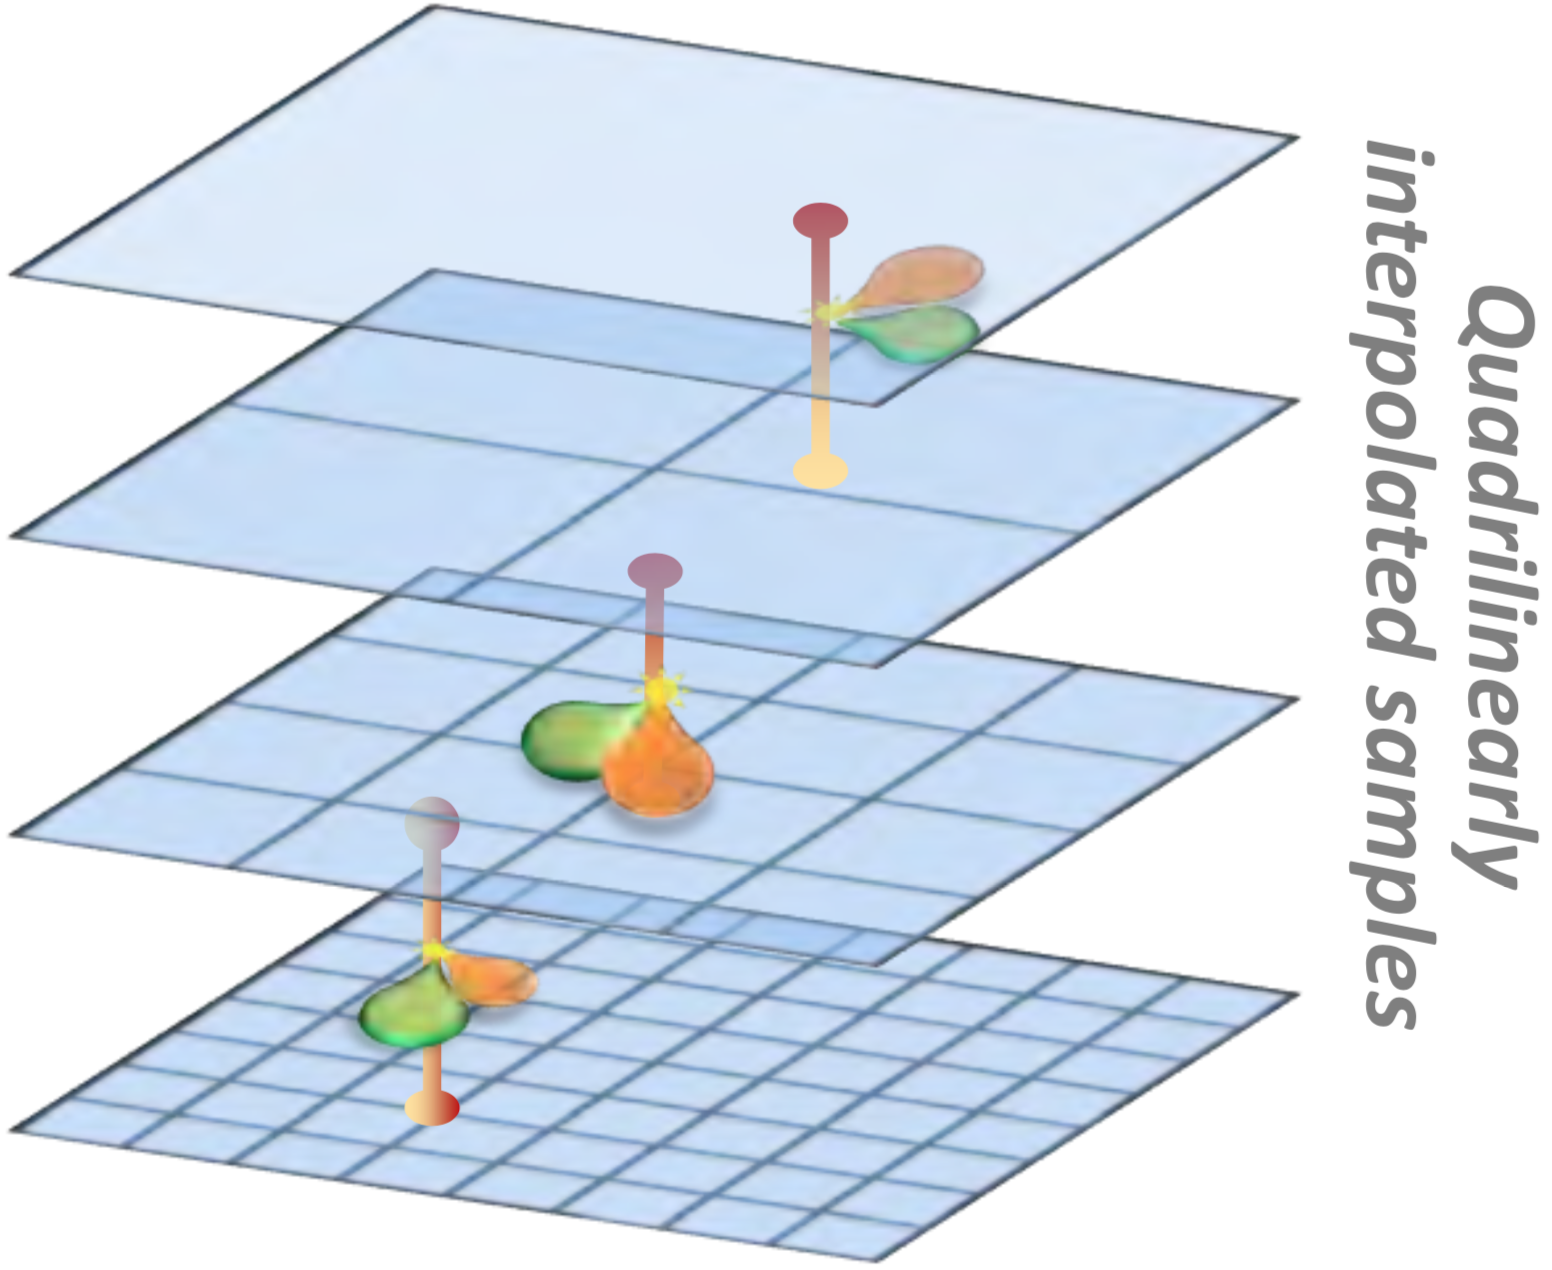
\includegraphics[width=0.45\textwidth]{figures/vct/vct-7-6}
	\caption{预积分能量函数 和预积分透明度函数中相关 值的多级结构,这种多分辨 率结构可以按照不同的细节 层次进行选择,其选择的依 据为预积分的长度(图片来自\cite{a:InteractiveIndirectIlluminationUsingVoxelConeTracing})}
	\label{f:vct-7-6}
\end{figure}

因此,我们可以在空间中选择一些离散的均匀分布的位置 $\mathbf{p}$,并在这些位 置计算这些函数的预积分值,这些预积分的长度 $l$ 对应了这些体素的尺寸,因 此可以用来决定多级体素的层级。由于我们希望使用正立方体结构的体素,所 以这个预积分长度 $l$ 可以与体素内表面的面积 $s$ 联系起来,即 $s = l^{2}$。较大像 素足迹将导致较长的预积分,这使得我们可以根据细节层次选择对应分辨率的 体素,其中像素足迹的(面积)大小充当了这种细节层次选择的索引值。

在上述的体素表述中,每个体素中存储的预积分透明度 $\overline{T}$ 对应的是从某个 方向看,该体素整个体积对应的截面的透明度;类似地,预积分的向内散射能 量 $\overline{Q}$ 则对应的是该体积内的表面沿某个方向过滤后的能量值。在实践中,我们 并不希望直接在体素中存储预积分能量值 $\overline{Q}$,相反,我们希望存储每个体素内 的表面对应的着色参数,以使我们可以在渲染时动态地计算 $\overline{Q}$ 的值。

\begin{figure}
\begin{center}
	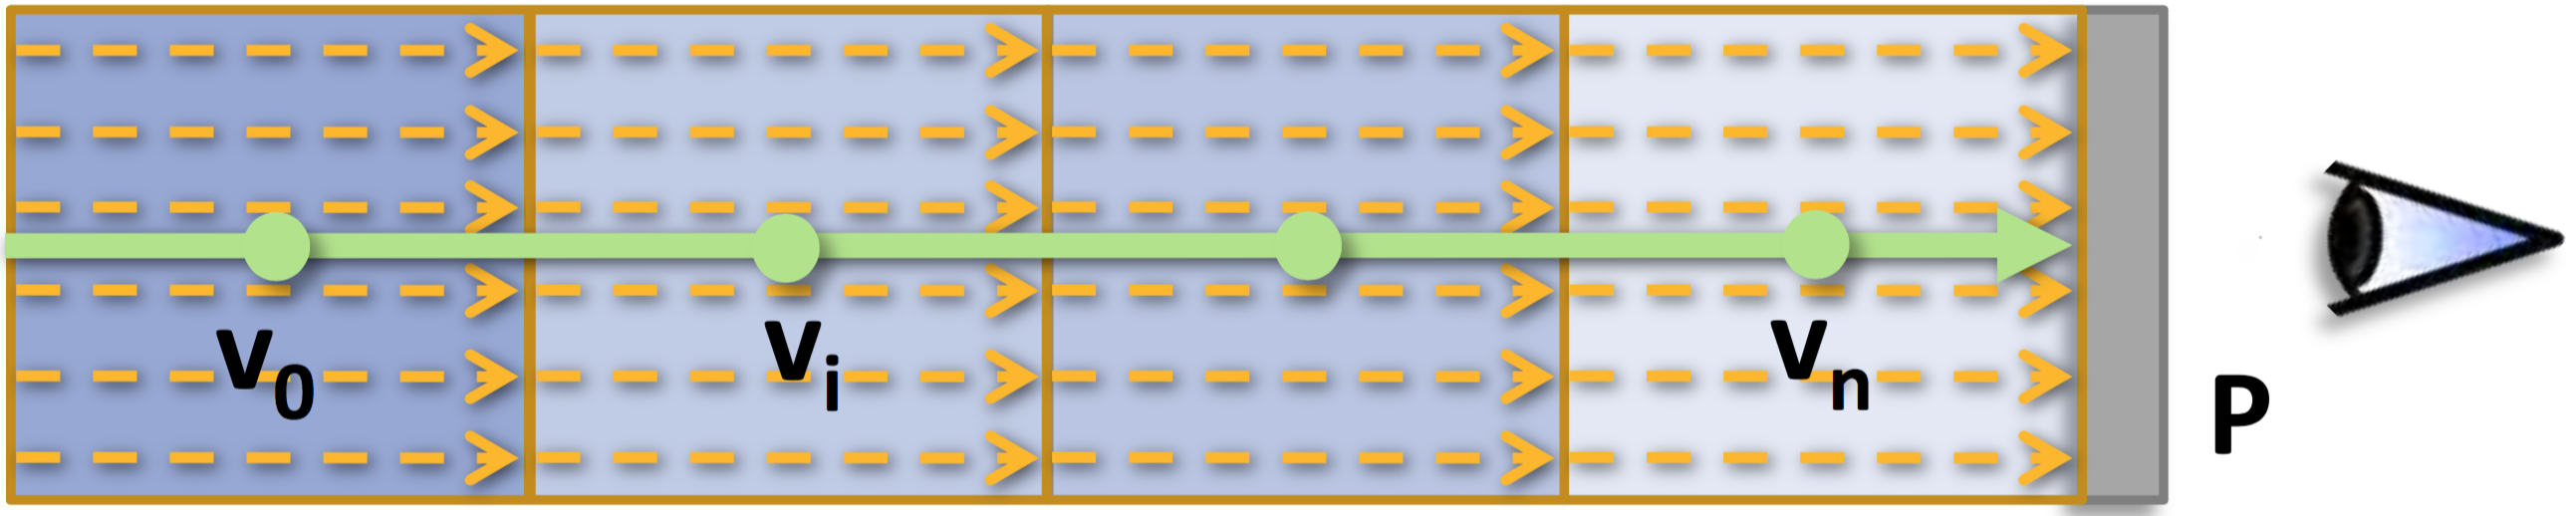
\includegraphics[width=0.8\textwidth]{figures/vct/vct-7-3}
	\end{center}
	\caption{对于一个给定像素,它沿着一条光线的能量可以表述为多个子体积内能量的累加, 其中每个子体积 Vi 内存储的是预积分的能量值,这些体积以多级体素的形式存储,渲染时 可以根据像素的足迹尺寸动态选择相应的分辨率(图片来自\cite{a:InteractiveIndirectIlluminationUsingVoxelConeTracing})}
	\label{f:vct-7-3}
\end{figure}

基于上述的表述,为了完整描述$\overline{Q}(\mathbf{p},\mathbf{d},s,l)$ 和 $\overline{T}(\mathbf{p},\mathbf{d},s,l)$,每个体素内 唯一需要存储的参数就只剩下积分的方向 $d$。



\subsubsection{四线性插值}\label{sec:vct-quadrilinear}
在渲染的时候,屏幕上的每个像素(沿着从摄像机到该像素的方向)发射 一条光线,沿着这条光线,我们对前面介绍的多级体素结构进行采样,在每个 采样的位置,该像素尺寸对应的表面面积 $s$ 被用于选择合适的细节层次,所有 采样得到的体素样本的光照贡献被累加起来形成对该像素总的光照贡献。

由于多级体素结构存储的是一些离散的函数值,因此上述采样使用的(连 续体积中的)位置 $\mathbf{p}$ 以及(连续足迹)面积 $s$ 的值需要从多级体素结构中的值 插值计算而出,本节我们将首先讨论怎样从多级体素结构中插值重建出任意连 续位置处的光照值。

对于一条光线,在垂直于该光线(即平行于屏幕)的平面上\footnote{该平面实际上可以看做多级体素结构中一个固定的层级。} ,光线与该平 面交点处的透明度 $\overline{T}$ 可以从该平面执行双线性插值计算出来。然而,这个预积分的透明度 $\overline{T}$ 在光线方向上却不是线性的,在这个方向上,根据体积渲染积分, 其透明度的变化是呈指数的,因此不能被线性插值\footnote{同样的线性插值问题页存在于向内散射能量 $\overline{Q}$ 中,即能量值在垂直于光线方向是线性的, 但是由于涉及可见性的积分,能量值在光线方向是非线性的。} 。然而,为了使用硬件提供 的三线性插值,这里直接对所有坐标轴方向使用线性插值,因此总的插值方法 称为四线性插值(quadrilinear interpolation)\myindex{四线性插值}{quadrilinear interpolation}。在大多数情境下,这种近似导 致的精度问题都是可忽略的。



\subsubsection{圆锥体形状的光束}
上面讨论的预积分模型仅仅计算像素沿光线方向平行投影产生的光束的体 积渲染积分,借助前面介绍的存储预积分能量和预积分可见性的多级体素结构, 现在我们将解释怎样近似由沿光线的透视投影产生的圆锥体形状的光束的体积 渲染积分。

在实践中,对于反走样,通常使用比较小的圆锥体光束,因此圆锥体光束 中的每个局部子体积可以近似看做一个正立方体,因此我们可以简单地使用沿光 线方向变化的细节层次来近似圆锥体形状的光束的体积渲染积分\footnote{但是对于较大的圆锥体,这种近似方法将导致采样不足,我们将在本章后面进一步讨论这 个问题。}。

这里的核心思路是,对于每一个体素样本,我们使用采样位置处对应圆锥 体截面的面积来作为层级细节的索引,这种采样方法的概念如图\ref{f:vct-7-4}所示,如前 面介绍的内容,由于多级体素结构只存储一些离散位置的值,因此我们必须对 两个相邻的体素层级中的值执行线性插值以计算任意连续面积处的光照值。

\begin{figure}
\begin{center}
	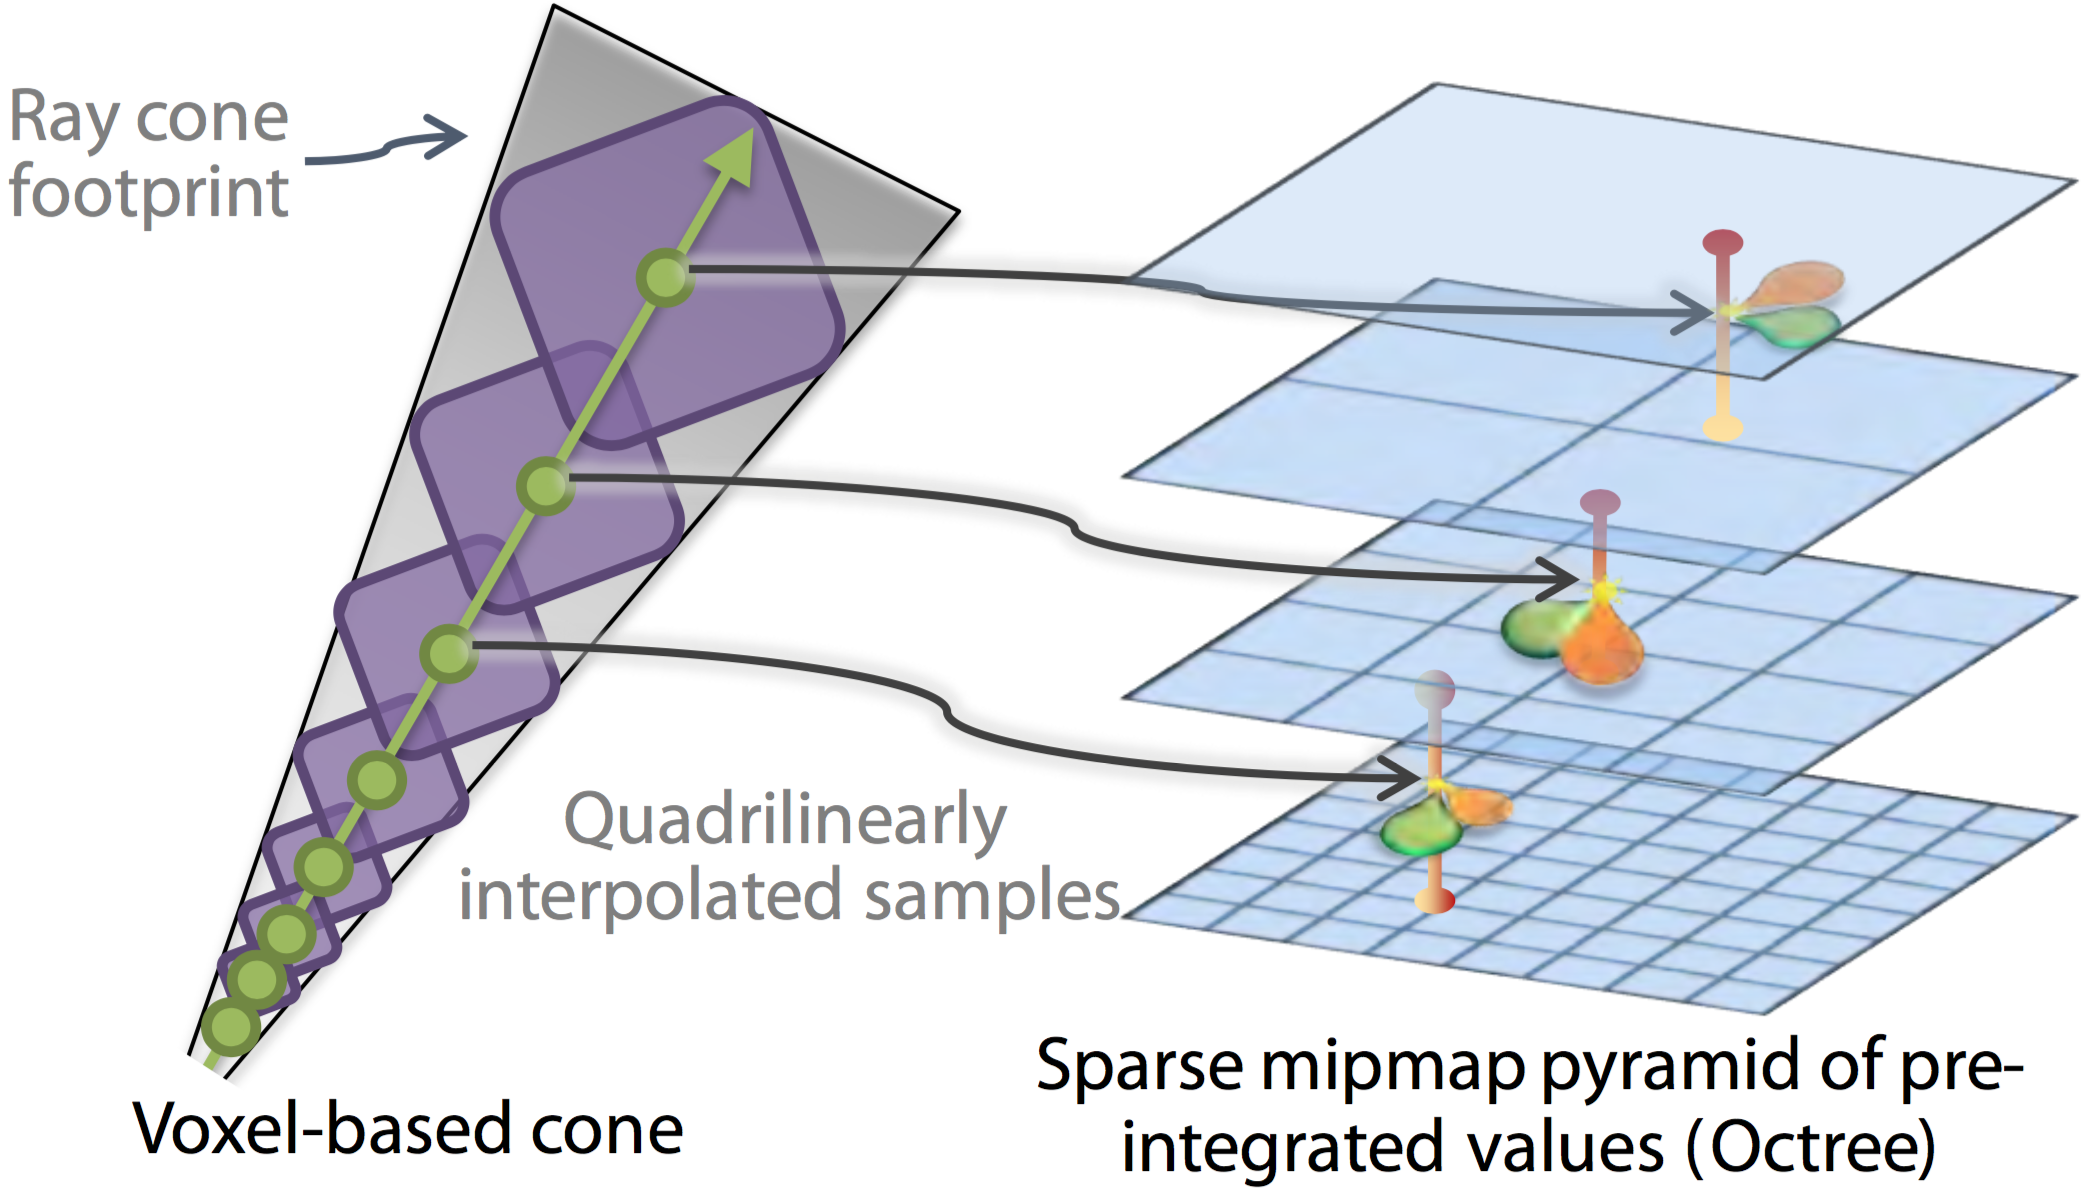
\includegraphics[width=0.75\textwidth]{figures/vct/vct-7-4}
\end{center}
	\caption{光线的透视投影产生了圆锥体形状的光束,该光束中的各个离散位置对存储预积分 值的多级体素结构进行采样,然后对其采样值进行四线性插值(图片来自\cite{a:InteractiveIndirectIlluminationUsingVoxelConeTracing})}
	\label{f:vct-7-4}
\end{figure}

在图\ref{f:vct-7-5}中,每个子体积内的预积分计算是按正交投影计算的,而我们期 望的是透视投影,这种简化使得圆锥体光束的每个局部子体积内存在一定的体 积被忽略,这种误差随着预积分体积的增加而增加。不过通常由于圆锥体孔径 比较小,这种误差是可以忽略的。

\begin{figure}
	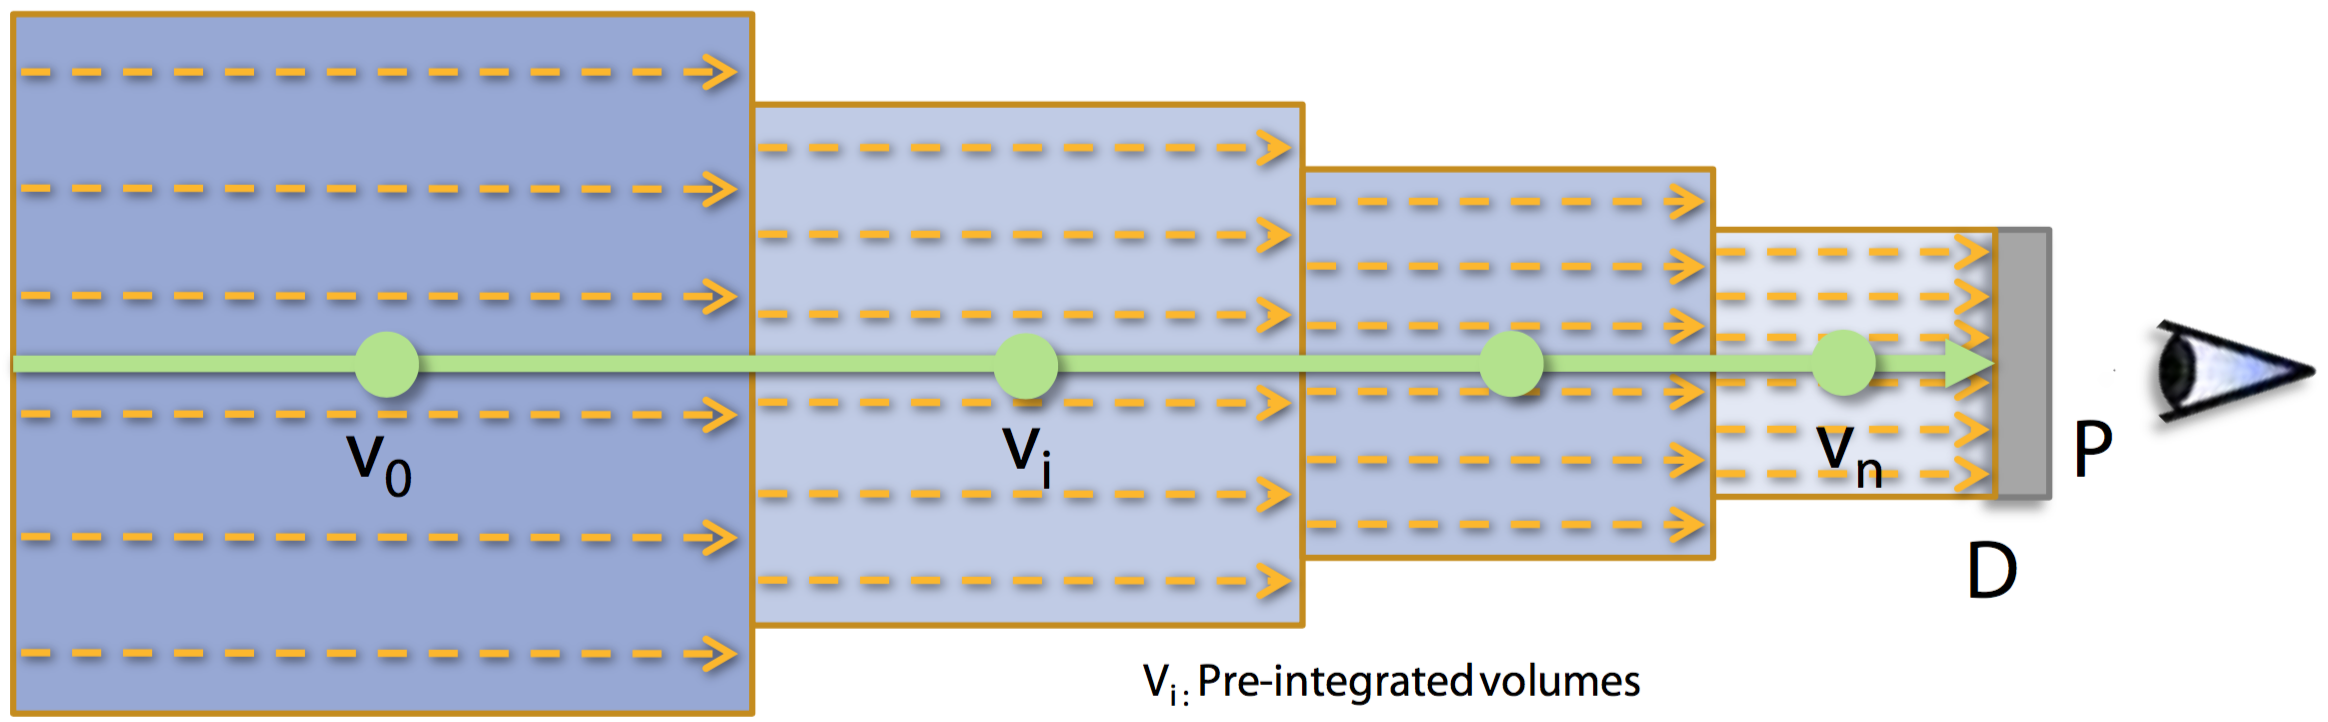
\includegraphics[width=\textwidth]{figures/vct/vct-7-5}
	\caption{光线的透视投影产生了圆锥体形状的光束,该光束中的各个离散位置对存储预积分 值的多级体素结构进行采样,然后对其采样值进行四线性插值(图片来自\cite{a:InteractiveIndirectIlluminationUsingVoxelConeTracing})}
	\label{f:vct-7-5}
\end{figure}



\paragraph{圆锥体足迹}
该模型的第二个近似来源于,我们使用了一连串与多级体素表述的坐标轴对齐的正立方体形状的体积去近似原本连续的圆锥体体积,如图\ref{f:vct-7-5}所示。

因为从多级体素中读取的数据会被执行四线性插值后用于光线的光照计 算,所以实际光线使用的足迹的精确度并不是非常重要。图\ref{f:vct-8}展示了光线 使用的具体足迹的分布,可以看到它们在一个体素空间内是固定的,这与实际的像素足迹具有一定的偏差,并且这种偏差随着体素分辨率的增大而增大。 图\ref{f:vct-8}(a) 展示了一个孔径为 $11.25^{\circ}$ 的圆锥体光线的足迹分布,图\ref{f:vct-8}(b) 的 圆锥体孔径则为 $22.5^{\circ}$,图\ref{f:vct-8}(c) 展示了这些足迹在 2D 空间的一个切面,可以看出,尽管单个圆锥体的足迹是呈块状分布的,但是实际上它们仍然能够近 似出一个以光线为中心的高斯分布。因此,当多条光束从相邻的像素发出时,这 种近似能够收敛至一个比较好的采样结果,这种采样实际上能够在全局空间内 保持能量守恒,图\ref{f:vct-8}(d) 展示了这种结果,一条线段上的所有像素发射出一 个系列光线,我们可以看出这得到了预期的结果,即体素光照的权重随着离屏 幕像素距离的增加而减少。

\begin{figure}
	\begin{subfigure}[b]{0.243\textwidth}
		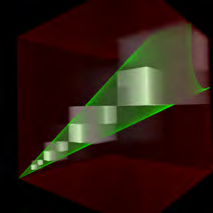
\includegraphics[width=\textwidth]{figures/vct/vct-8-1}
		\caption{}
	\end{subfigure}
	\begin{subfigure}[b]{0.243\textwidth}
		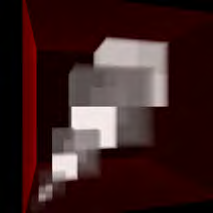
\includegraphics[width=\textwidth]{figures/vct/vct-8-2}
		\caption{}
	\end{subfigure}
	\begin{subfigure}[b]{0.243\textwidth}
		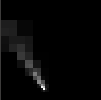
\includegraphics[width=\textwidth]{figures/vct/vct-8-3}
		\caption{}
	\end{subfigure}
	\begin{subfigure}[b]{0.243\textwidth}
		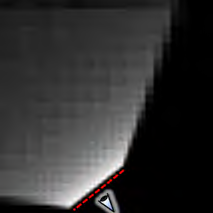
\includegraphics[width=\textwidth]{figures/vct/vct-8-4}
		\caption{}
	\end{subfigure}
	\caption{图示了在预积分的体素内光线的足迹形状,可以看到它们并没有反应光线的真实足迹分布,其中,(a)和(b) 分别在3D空间中展示了两个不同圆锥天顶角度的足迹分布,(c) 展示了 3D 足迹的一个 2D 切面,(d) 展示了沿着一条直线上所 有像素的多个足迹的分布(图片来自\cite{a:InteractiveIndirectIlluminationUsingVoxelConeTracing})}
	\label{f:vct-8}
\end{figure}




\subsection{预过滤的着色参数}
本章前面的内容假设体素表述中的反射能量已经存在,我们讨论了怎样使 用这些来自体素中的预积分数据(例如平均向内散射能量 $\overline{Q}$ 和平均透明度 $\overline{T}$) 来计算光线的光照贡献,即根据式\ref{e:vct-pre-intergation}来累加光线步进中各个位置处对应细节 层次的体素的光照贡献,这种累加的模型来源于对体积渲染积分的近似。本节 我们将聚焦于每个体素怎样存储这些预积分数据。

在式\ref{e:vct-pre-intergation-item}中,我们假设对于每个像素沿某个方向发出的光线,该光线每个 位置处的光照能量全部已经被预积分到数据 $\overline{Q}$ 中,这就要求每个体素中需要存 储非常高维(这里是 8D 的函数)的数据,因为它需要考虑光线的方向,积分的 位置,长度以及面积等维度,例如在同一个位置处,不同的光线方向需要存储 不同的预积分数据,这显然是非常复杂的。为了允许完全动态的光照计算,本 节我们将介绍怎样将预积分 $\overline{Q}$ 中的光照信息从积分中提取出来,然后让预积分 仅计算材质相关的参数,而由于材质参数的线性特征,这种分离将前面的预积 分模型转换为了一个预过滤模型,这不光使得各个分辨率下的材质参数能够被 快速(预过滤)计算,而且还能够动态处理任意光照。

对于给定一个细节层次中的每一个体素,该体素的数据必须能够表述低于 该级的所有体素所对应的几何表面(即该体素所代表的所有表面面积)的光照 行为。如本书前面的内容所知,纹理预过滤技术的本质是,基于线性的假设,我 们能够从着色积分中分解出着色参数,并对这些着色参数进行预过滤,以实现 对渲染结果的反走样。这种操作的前提是分解出的着色参数与最终的渲染结果 是呈线性关系的。在本节下面的内容中,我们也将基于同样的理论,对体素预 积分中着色参数相关的部分进行分解,使之可以仅对着色参数信息进行预过滤, 从而能够在渲染时实现动态光照的计算。

具体来说,体素中会存储四类信息:体素内表面的透明度,漫反射材质颜 色,法线分布和 BRDF 分布函数,如图\ref{f:vct-9-1}所示,第\ref{sec:vct-local-shading}节则会讨论这些 体素数据怎样被用于表面像素的着色计算。然而我们并不会在本节讨论所有这 些参数,而是首先单独讨论与与材质相关的参数,即漫反射颜色和法线分布,这 种区分的原因主要之一是,我们要明白这两种参数与最终预积分结果的线性关 系,这使得前面介绍的预积分被转变为一个预过滤的形式,因此我们便可以直 接对材质参数进行预过滤,而不需要与光照能量一起计算整个预积分,这个结 果其实和传统的纹理过滤是相似的,这使得预积分中的光照能量与材质参数分 离,这样最终整个预积分才可能重用材质参数预过滤的结果,这是本章讨论的 基于体素的全局光照技术能够提升效率的一个关键原因,这也和传统的着色渲 染中表面能够任意使用预过滤的多级纹理是一个道理。其它的表示遮挡关系的 透明度以及 BRDF 分布函数则将留在后面第\ref{sec:vct-implementation}节进行讨论。

\begin{figure}
\sidecaption
	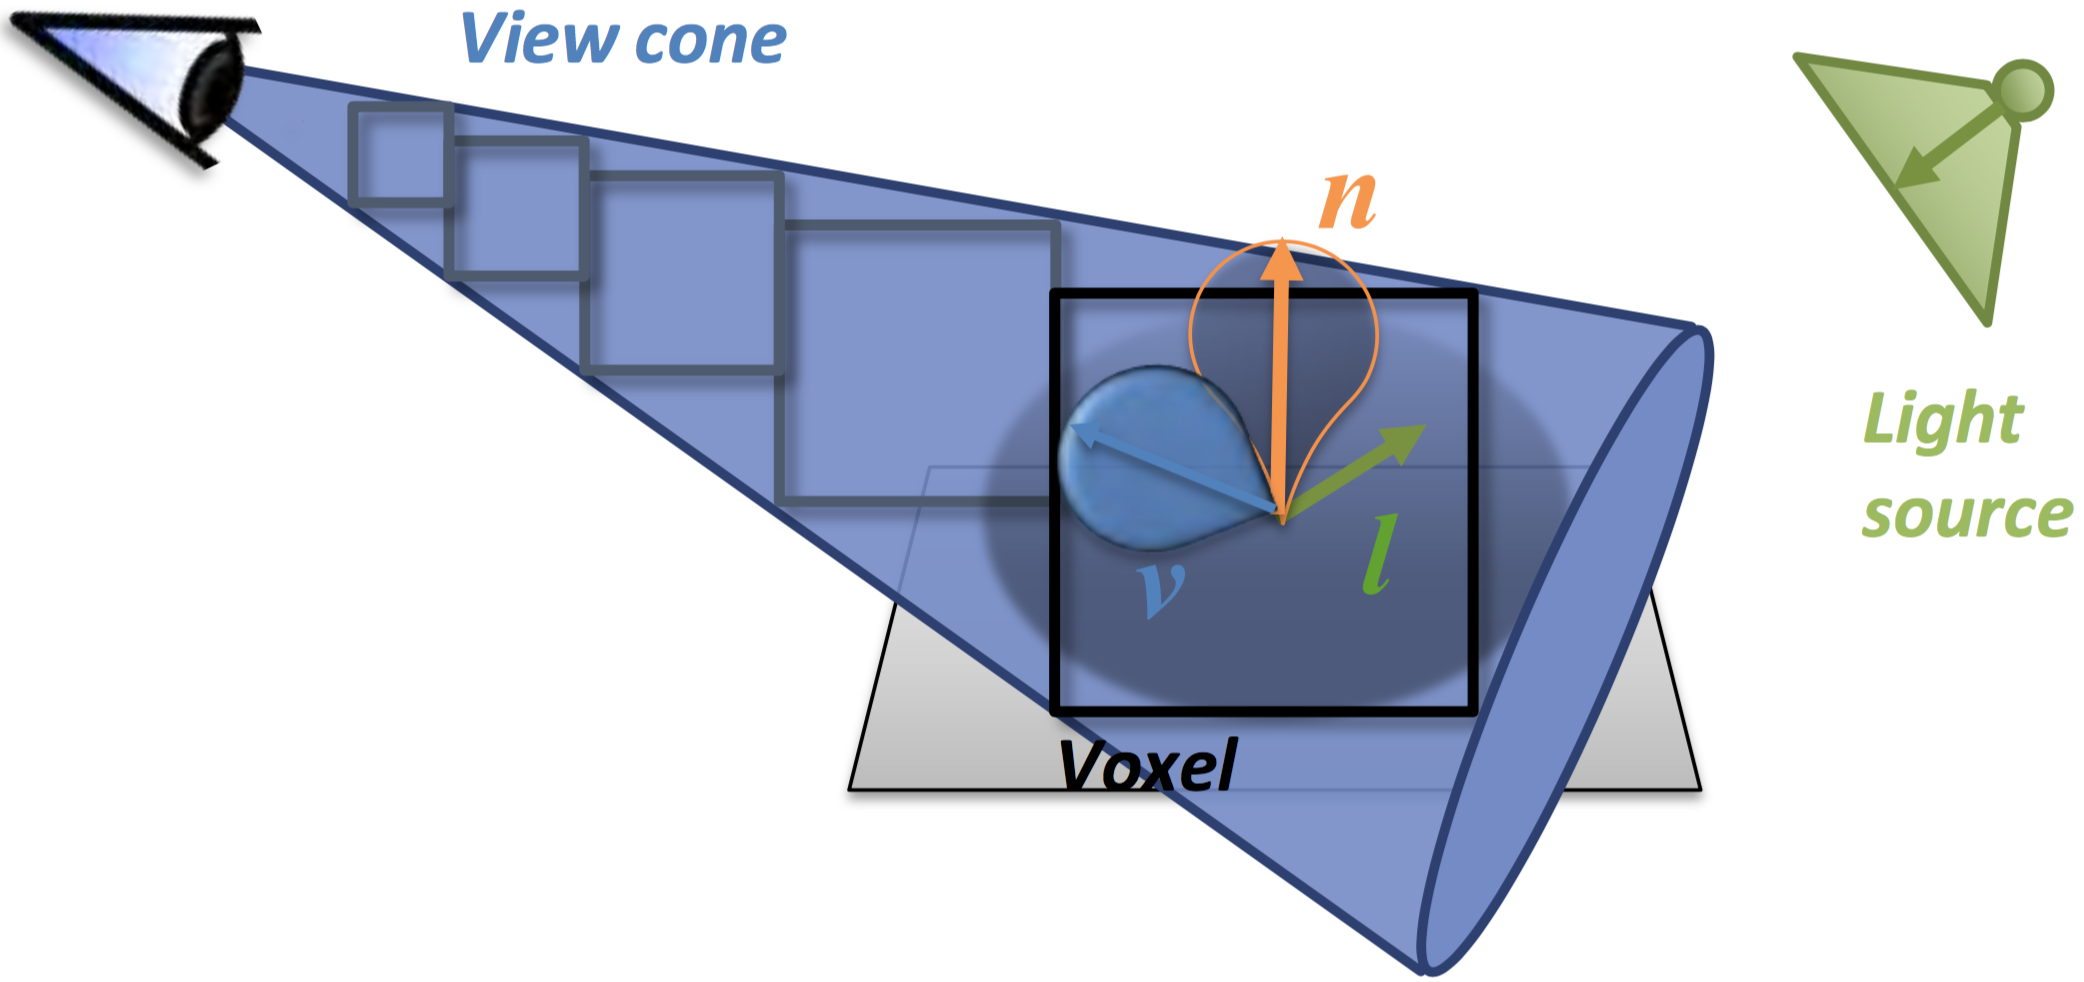
\includegraphics[width=0.65\textwidth]{figures/vct/vct-9-1}
	\caption{体素仅计算并存 储对表面材质参数进行预积 分的数据信息,由于这些参 数与最终积分值呈线性关 系,因此可以被预过滤(图片来自\cite{a:InteractiveIndirectIlluminationUsingVoxelConeTracing})}
	\label{f:vct-9-1}
\end{figure}



\subsubsection{漫反射颜色}
表面的漫反射颜色是直接存储在纹理中的,这不同于光泽反射,其形式被存储于BRDF反射函数中。反射方程中的漫反射部分是最简单的情形,因为材质的漫反射颜色是与最终的渲染结果呈线性关系的,所以可以直接将它从着色方程中分解出来并执行单独的预积分计算。漫反射颜色的积分和传统的纹理 预过滤的思路类似,即每个像素存储单个颜色值,所以直接对每个体素存 储一个预积分的漫反射颜色值 $\overline{C}_{RGB}$,它是对该体素内所有表面漫反射颜色执 行预积分的结果,然后我们再对下一级体素中的漫反射颜色值执行预积分以 构建一个多级体素结构。

由于这种线性关系,可以用过滤的方式来计算预积分,因此原始的(包含光照能量的非线性的)预积分模型被转化为一个(仅包含材 质参数的线性的)预过滤模型。所以当后面在讨论这些仅与材质相关的具有线性关系的参数时,通常是指预过滤,而其它参数如可见性,则它们还是使用的预积分模型,即它们每个地方都要根据实际的情 况执行积分计算,而不是能够使用一个核函数对任意位置执行简单的过滤操作,因为这些参数和最终积分结果并没有线性关系。



\subsubsection{法线方向信息}
对于表面的法线,这些信息会比漫反射颜色要更复杂。

首先需要考虑的是怎样表述一个体素的法线信息,每个体素仅存储单个平 均法线值肯定是不行的,因为那样将忽略掉体素内表面法线的变化(variation),因此需要对每个体素存储一个法线分布函数。我们已经在本书第一章中介绍了关于一个像素内微面元的法线分布函数,它和这里讨论的概念其实是一致的,法线分布函数(normal distribution function,NDF)\myindex{法线分布函数}{normal distribution function}是指一个表面上的所有点的法线在每个方向上的密度分布,因此它只是一个方向函数,它的值表明每个方向上法线的密度是多少,或者说给定任意一个表面上的点,它有多少概率指向某个方向。

那么我们为什么需要法线分布函数呢?在传统的光照模型中,表面上的每 个点(或像素)被指定一个法线方向,它表明该像素面的朝向,如果该面是绝 对光滑的,那么对于每个入射方向该像素只有一个反射方向,但是如果该面内 的微观结构具有一定的粗糙度,则这些微面元就会形成一个法线分布函数,这 是第一章介绍的关于微面元理论的基本概念。从这里我们可以看出,法线分布 函数的存在是因为着色尺寸的尺度(这里即是一个像素大小)要大于表述表面 细节的尺度(即一个微面元的尺度)。那么将这种概念放在本章的上下文中,这 里采样的尺度是一个体素,它显然要大于表述表面细节的那些表面分布,因此 对于这样的一个体素的着色计算,我们需要一个表述该体素内微观结构的法线 分布函数,而不是对于每个体素仅存储单个法线值,因为那样就会忽略掉体素 内的细节,就如同对一个像素的着色计算忽略了微面元的细节,体素的法线分 布函数如图\ref{f:vct-9-1}所示。

其次,对于每个体素内的法线分布函数,我们需要考虑的另一个重要问题是怎样对这个法线分布函数执行预过滤操作,因为一个简单的使用矢量表述的表面法线分布(例如传统的使用纹理表述的表面法线)与着色结果并不是线性关系,即我们不能通过简单地对周围相邻的法线矢量做平均计算以对法线进行过滤,例如对来自相邻两个像素的两个法线方向的作平均值计算,其结果是另一个法线方向,它反映不出其平均的两个像素的法线细节。

我们需要一种对一个法线分布函数执行过滤,其结果仍为一个法线分布函 数的过滤模型。传统的对法线贴图进行过滤的方法是基于这样的思路,即使用一个能够被线性过滤的统计分布模型来表述一个表面的法线方向分布,然后将 这些方向存储在法线贴图中,进而对其进行过滤。例如在\cite{a:Normaldistributionfunctionsandmultiplesurfaces,a:Frequencydomainnormalmapfiltering}中,法线分布函数的过滤通常转化为法线分布函数与 BRDF 分布 函数的一个卷积计算,这些方法使用的一些比较精确的法线发布函数如球谐函 数等,这样的分布函数用在本章讨论的基于体素的全局光照模型中虽然是可行 的,但是这些球谐函数系数却会占据较大的内存。

\cite{a:Mipmappingnormalmaps}指出,对两个归一化的法线求平均值,其得到的“平均法线”的长度通常小于 1,除非这两个法线是完全相同的,尽管这个平均值法线不能反映被平均的两个法线的细节,但是可以使用这个平均值法线的长度作为一个高斯分布的标准偏差 $\sigma$ 的度量,这样的一个高斯分布则可以用来近似平均后的法线分布函数。\cite{a:Gigavoxels:Avoxelbasedrenderingpipelineforefficientexplorationoflargeanddetailedscenes,a:InteractiveIndirectIlluminationUsingVoxelConeTracing}采用了这种简单的近似模型,其中每个体素只需要存储一个平均法线矢量 $N$,该平均法线对应的法线分布函数为一个高斯分布,其方差可以使用该平均法线的范数 $|N|$ 来计算,即 $\sigma^{2} =\cfrac{ 1−|N|}{|N|}$。



\subsubsection{局部着色模型}\label{sec:vct-local-shading}
通过上一节的内容可知,由于每个体素内并没有直接存储预积分能量值 $\overline{Q}$, 而只是存储了一些被预过滤后的材质参数,例如漫反射颜色 $\overline{C}_{RGB}$,法线平均 值 N,这种处理的目的是为了能够实时动态地计算不同的光照,然而这也要求 每个体素内实际$\overline{Q}$ 需要在采样的时候实时地被计算出来。

我们的目标是对于一个给定的体素,及其存储的漫反射颜色 $\overline{C}_{RGB}$,预过 滤的法线分布函数 $\overline{N}$ 以及该体素的体积扩展范围到摄像机和光源的那些方向 集合,计算出该体素对像素的光照贡献。当然这里忽略了体素的可见性,因为 体素的可见性已经被从体素的光照能量计算中分离出来,它仅被用于对体素最 终的光照结果做一个类似透明度的混合处理。因此我们又称这种单个体素的着 色模型为局部着色模型。

为了推导出这个局部着色模型,我们从最基本的反射方程(reflectance equation)开始,在表面上点 ${x}$ 处沿 $\omega_o$ 方向的反射光照为:


\begin{equation}\label{e:vct-reflection-equation}
	L({x},\omega_o)=\int_{S^{2}}L({x},\omega_i)\rho(\omega_i,\omega_o;\mathbf{n}({x})){\rm d}\omega_i
\end{equation}

这里 $\rho$ 表示表面的 BRDF 分布函数(其包含了余弦函数几何项),注意这里没有区分辐射亮度 $L$ 的方向,在本节的上下文中,$L({x},\omega_o)$ 始终表示出射光照,而 $L({x},\omega_i)$表示入射光照。在上式中,我们需要围绕整个半球面 $S^{2}$ 计算该积分。

式\ref{e:vct-reflection-equation}表示的是对于单个点 ${x}$ 处的反射光照的计算,对于该单个点,我们 有且仅有一个法线值 $\mathbf{n}({x})$。然而对于一个体素,它表述的是其体积包含的多个 表面位置的集合,而不再是单个表面点,其中这些包含的表面的法线位于一个 法线分布函数中,假设这些点的集合为 $q \in {x}$,则整个体素内反射光照的值可 以表述为所有点 $q$ 处反射光照值的平均值,即:

\begin{equation}\label{e:vct-reflection-equation-1}
\begin{aligned}
	L({x},\omega_o)=&\cfrac{1}{N}\sum_{q\in {x}}\int_{S^{2}}L({x},\omega_i)\rho(\omega_i,\omega_o;\mathbf{n}(q)){\rm d}\omega_i\\
	=&\int_{S^{2}}L({x},\omega_i)\Biggl(\cfrac{1}{N}\sum_{q\in {x}}\rho(\omega_i,\omega_o;\mathbf{n}(1))\Biggl){\rm d}\omega_i
\end{aligned}
\end{equation}

注意在上式的推导中,这里隐含假设了光照是不随 $p$ 位置的变化而变化的, 我们仅考虑表面的法线变化,因为这些变化对反射光照的影响更大。根据上式, 我们可以重新定义一个针对体素(而不是像素)的 BRDF 分布函数,即:

\begin{equation}\label{e:vct-voxel-distribution}
	\rho_v(\omega_i,\omega_o;{x})=\cfrac{1}{N}\sum_{q\in {x}}\rho(\omega_i,\omega_o;\mathbf{n}(q))
\end{equation}

在上式中,${x}$ 表示的是一个体素(而不是某个像素的)的位置,如图\ref{f:vct-9-2}所示。不难看出,该 BRDF 函数的值隐式地由体素位置 ${x}$ 处的法线分布函数 $\mathbf{n}(q)$ 决定(这个法线分布函数实际上是近似的体素内所有细节表面的法线分布),而 不是像式\ref{e:vct-reflection-equation}中由单个法线值决定。

\begin{figure}
	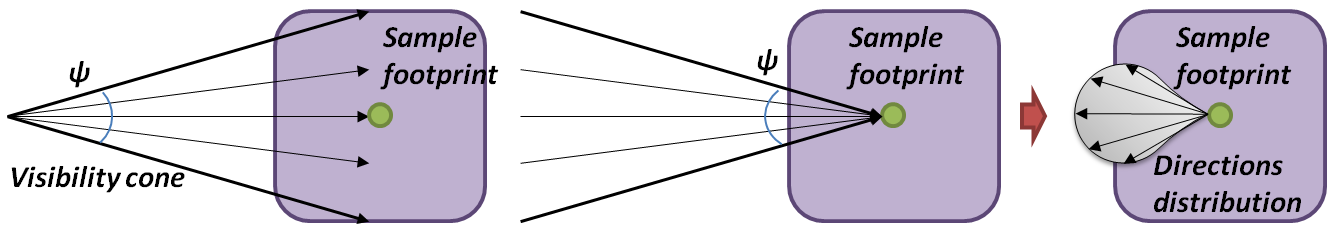
\includegraphics[width=\textwidth]{figures/vct/vct-9-2}
	\caption{一个表面参数被预过滤的体积的方向分布,由此可以看出一个体素不同于单个像素, 它需要计算多个表面位置的反射光照,即是要围绕一个法线分布函数进行积分计算(图片来自\cite{a:InteractiveIndirectIlluminationUsingVoxelConeTracing})}
	\label{f:vct-9-2}
\end{figure}

那么剩下的问题就是怎样高效地计算 $\rho_v$呢?式\ref{e:vct-voxel-distribution}是一个离散的函数,它 是对所有离散位置 $q$ 的一个平均值计算,假设这些位置都是连续的,我们可以 将其转换为一个连续的积分形式\cite{a:Frequencydomainnormalmapfiltering},即:

\begin{equation}\label{e:vct-voxel-distribution-1}
	\rho_v(\omega_i,\omega_o;\gamma(\cdot))=\int_{S^{2}}\rho(\omega_i,\omega_o;\mathbf{n})\gamma(\mathbf{n}){\rm d}\mathbf{n}
\end{equation}

这里 $S^{2}$ 表示体素内所有表面的法线方向,$\gamma(\mathbf{n})$ 即表示体素的法线分布函 数,每个体素位置 ${x}$ 存储这一个唯一的法线分布函数 $\gamma(\mathbf{n})$。

通过式\ref{e:vct-voxel-distribution-1}可以看出,体素的 BRDF 分布函数 $\rho_v$ 可以转化为原始表面上基于像素的 BRDF 分布函数 $\rho$ 和体素位置 ${x}$ 处法线分布函数 $\gamma(\mathbf{n})$ 的卷积。其中体素的法线分布函数已经被使用一个平均法线 $|N|$ 表述为一个高斯分布,其方差为 $\sigma^{2}_n = \cfrac{1−|N|}{|N|}$ ,如果考虑简单的冯氏模型,即表面的 BRDF 分布也可以表述为一个高斯分布,根据\cite{a:Mipmappingnormalmaps},平面上两个标准偏差为$\sigma$  和 $\sigma_s$ 的高斯分布,其卷积为一个标准偏差更大的高斯分布,该高斯分布的方差为$\sigma^{2}_{s^{'}}=\sigma^{2}+\sigma^{2}_s$,以此我们可以很高效地计算出一个体素的BRDF分布函数$\rho_v$,最后将该体素的分布函数代入式\ref{e:vct-reflection-equation-1}即可按照传统的反射方程计算出体素的出射能量。除此之外,我们仍然可以使用其它 BRDF 模型,这里只是一个不同的卷积计算而已。

在上面的讨论中,我们将体素看做一个“点”,然后其积分方向是围绕该点来 展开的,如图\ref{f:vct-9-2}中间小图所示,但实际上体素的光照积分方向应该是从摄像机发 出的,然后求与体素内的表面相交处的反射光照,如图\ref{f:vct-9-2}左边小图所示,可以看 出这两种方向分布的计算结果是一样的。

最后,为了更好的对体素内各个表面位置处的光照结果进行平滑处理,即 更好地实现反走样,我们并不是像式\ref{e:vct-voxel-distribution}那样直接取所有表面位置处反射光照 结果的平均值,而是对这些结果执行了一个过滤处理,如图\ref{f:vct-9-2}右边小图所示,这 里使用了一个高斯分布核函数,其标准偏差为$\sigma_v= \cos(\psi)$,这里 $\psi$ 表示体素 到摄像机形成的圆锥体孔径的角度。




\subsection{实~~现}\label{sec:vct-implementation}
本节最后再来总结整理关于体素的表述和实现方案,我们的目标是对多级 体素(我们将在后面第\ref{sec:vct-data-structure}在详细讨论这种多级体素的数据结构以及在 GPU 中的遍历算法)中最高分辨率层级中的每个体素,存储一个平均漫反射颜色值 $C_{RGB}$,一个法线分布函数 $N$ 以及一个透明度 $T$。最后我们将对多级体素的最 高分辨率层级进行过滤和预积分计算,以得到整个多级体素的金字塔结构,其 中具体的预过滤或预积分方法也会留在下一节讨论,因为它涉及到多级体素的 数据结构,并且这个过程发生于多级体素的构建过程当中。

上一节已经介绍过与材质参数相关的项,由于具有线性关系,这些参数可 以被直接使用预过滤处理,然而透明度则不同,体素的透明度通常与光照结果 不具备线性关系,因此透明度需要使用预积分的方式进行计算。由于预积分计 算会更加复杂,所以通常会使用更加近似的方法。

对于多级体素最高分辨率层级中的每个体素,我们用体素内所有与之相交 物体的联合(union)的体积占总体素体积的密度 $\rho$ 来近似该体积的可见性,同 时还需要考虑这些物体本身的透明度,这里用一个平均吸收系数 $\kappa^{'}$  来表述,它 仅仅是所有相交物体透明度的平均值。加入对 $\kappa^{'}$ 的计算使得我们可以表述和 过滤半透明的物体,最终得到一个加权的吸收系数为 $\kappa =\kappa^{'} \rho$,这个系数被用 于计算每个体素最终的平均透明度 $T = {\rm e}^{-\kappa\Delta x}$ ,其中 $\Delta x$ 表示体素的尺寸。

另一方面,在计算体素内材质的平均颜色 $C_{RGB}$ 时,其中每个参与平均计 算的物体的漫反射颜色还需要被使用一个因子进行缩放,该因子表述的是该单 个物体在体素内的密度与体素总的密度 $\rho$ 的比例,这样可以调整每个物体的颜 色贡献权重。类似的,每个参与平均法线值 $N$ 计算的法线也需要被该因子缩放, 这里可能看起来有点不好理解,法线只不过是一个方向矢量,有什么可以缩放 的呢?这里主要是因为体素最终的法线分布函数是与平均法线值的长度 $|N|$ 相 关的,因此被缩放的法线能够影响每个物体对最终法线分布函数的贡献权重。

在实践中,颜色值 $C_{RGB}$ 和透明度 $T$ 通常被合并存储为一个 $RGBA$ 颜 色矢量,其中不透明性分量 $\alpha = 1 − T$ ,其 RGB 颜色分量记录的是使用不透 明性加权的颜色值 $RGB =\alpha C_{RGB}$。法线分布函数存储为一个简单的 3D 矢量 $N_{xyz}$,该矢量仍然考虑了 $\alpha$ 的预乘,以提供更好的插值计算。

在第\ref{sec:vct-mip-pre-intergation}节介绍的预积分多级体素模型中,定义一个体素内预积分的方 向的参数 $\mathbf{d}$ 目前并没有被考虑,以下提供两种实践性的实现用于处理这个参数 的离散化,其中第一种实现完全忽略这个方向维度,而是对每个体素仅存储一 些各向同性的值,第二种模型则提供一种对各向异性参数值的简单进行,它基 于在各个坐标轴方向上对方向参数 $\mathbf{d}$ 进行离散化。图\ref{f:vct-12}显示了这两种模型渲染结果的对比。

\begin{figure}
	\begin{subfigure}[b]{0.5\textwidth}
		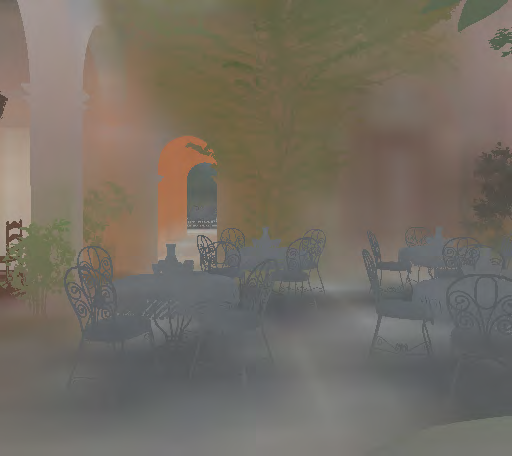
\includegraphics[width=\textwidth]{figures/vct/vct-12-1}
		\caption{}
	\end{subfigure}
	\begin{subfigure}[b]{0.5\textwidth}
		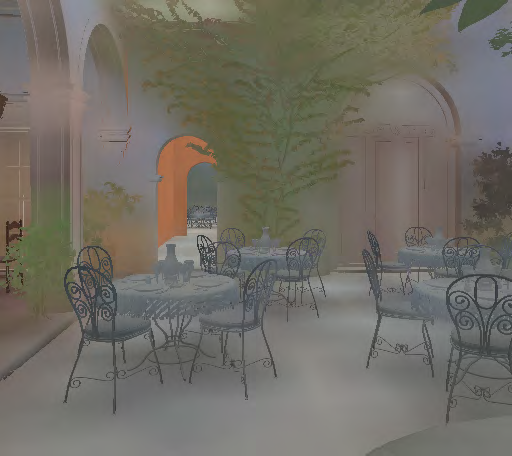
\includegraphics[width=\textwidth]{figures/vct/vct-12-2}
		\caption{}
	\end{subfigure}
	\caption{各向同性(a)和各向异性(b)两种模型渲染的结果对比(图片来自\cite{a:InteractiveIndirectIlluminationUsingVoxelConeTracing})}
	\label{f:vct-12}
\end{figure}


\subsubsection{紧凑的各向同性体素}
各向同性体素表述的优点是它的紧凑性,因为体素需要记录的每个参数都 只需要存储单个值即可。

这种表述只是前面介绍的理论预积分模型的一种非常粗略的近似,其多级 体素金字塔结构采样从最高的分辨率开始,从上至下的构建。在预计算体素内 实际的参数 $\overline{T}$,$\overline{C}_{RGB}$ 和 $\overline{N}$ 的值时,这些预积分模型内的可见性被完全忽略,这实际上和传统的多级纹理的方案类似,因为在计算每个像素的纹素值时,它并没有可见性需要考虑。为了计算多级体素当中低分辨率层级的体素,我们仅仅对其上一级体素中的参数执行简单的平均值计算即可。

尽管这种近似非常粗略,但是对于那些孔径很小的圆锥体,这种近似的结 果其实非常好。但是,对于那种较大空间的圆锥体,这种近似的结果就比较差, 如图\ref{f:vct-12}所示。




\subsubsection{增强的各向异性体素表述}
上述各向同性模型的第一个问题是,考虑两个红-绿墙的问题,如图\ref{f:vct-11}所 示,由于在体素中我们依赖于使用平均值来表述预积分值,在这种方法下,当 两个具有不同颜色值且不透明的体素被执行平均计算时,其混合的结果等效于 两个半透明的颜色值的和,如图\ref{f:vct-11}(c) 所示;同样的问题发生于对透明度的 计算,对于一系列 $2\times 2\times 2$ 的体素,其中一半的体素是不透明的,而另一半体 素是完全透明的,其混合后的结果则是半透明的。

\begin{figure}
\begin{fullwidth}
	\begin{subfigure}[b]{0.33\thewidth}
		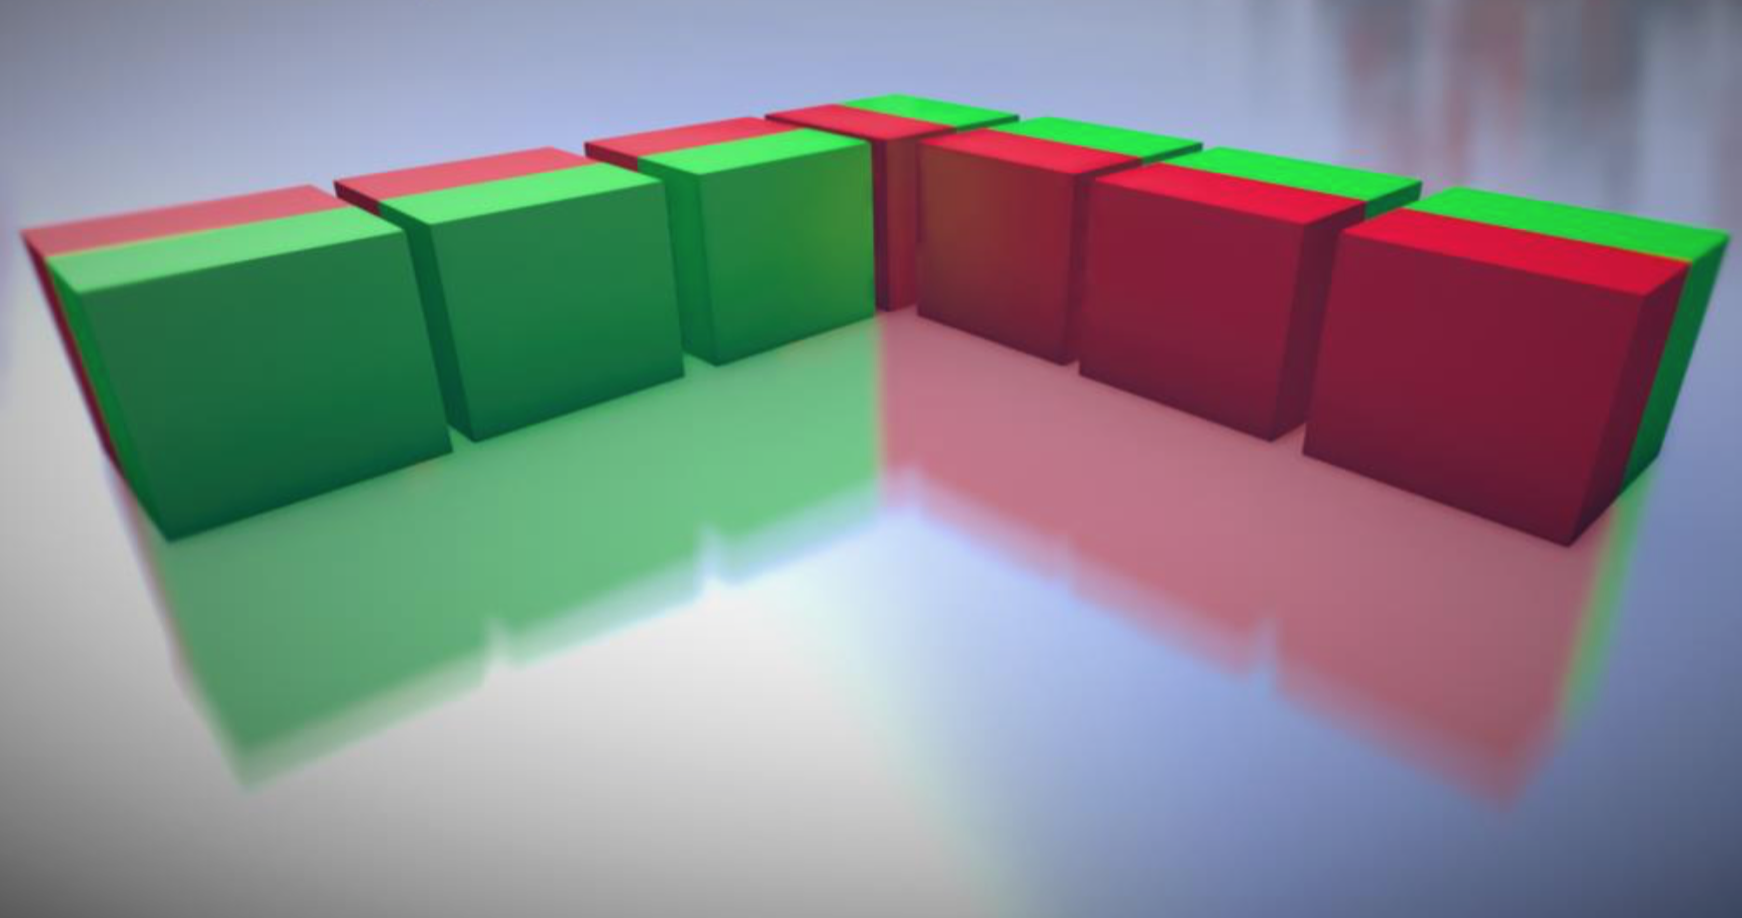
\includegraphics[width=\textwidth]{figures/vct/vct-11-2}
		\caption{多种颜色混合的体素}
	\end{subfigure}
	\begin{subfigure}[b]{0.33\thewidth}
		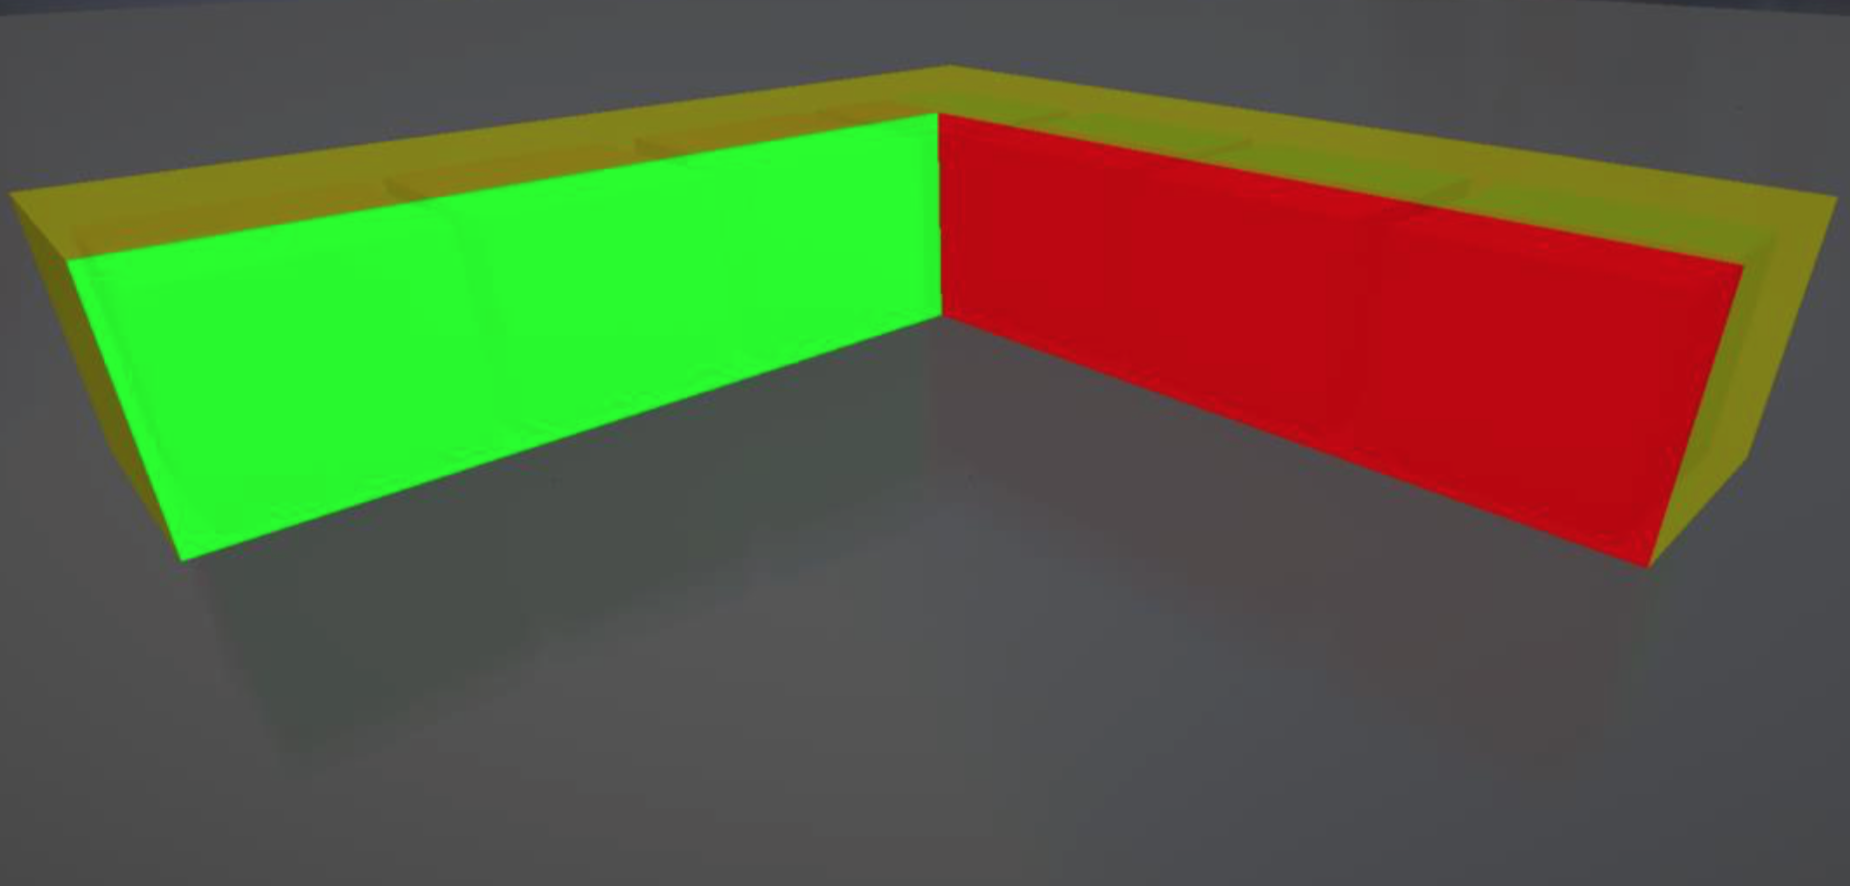
\includegraphics[width=\textwidth]{figures/vct/vct-11-3}
		\caption{各向异性混合的体素}
	\end{subfigure}
	\begin{subfigure}[b]{0.33\thewidth}
		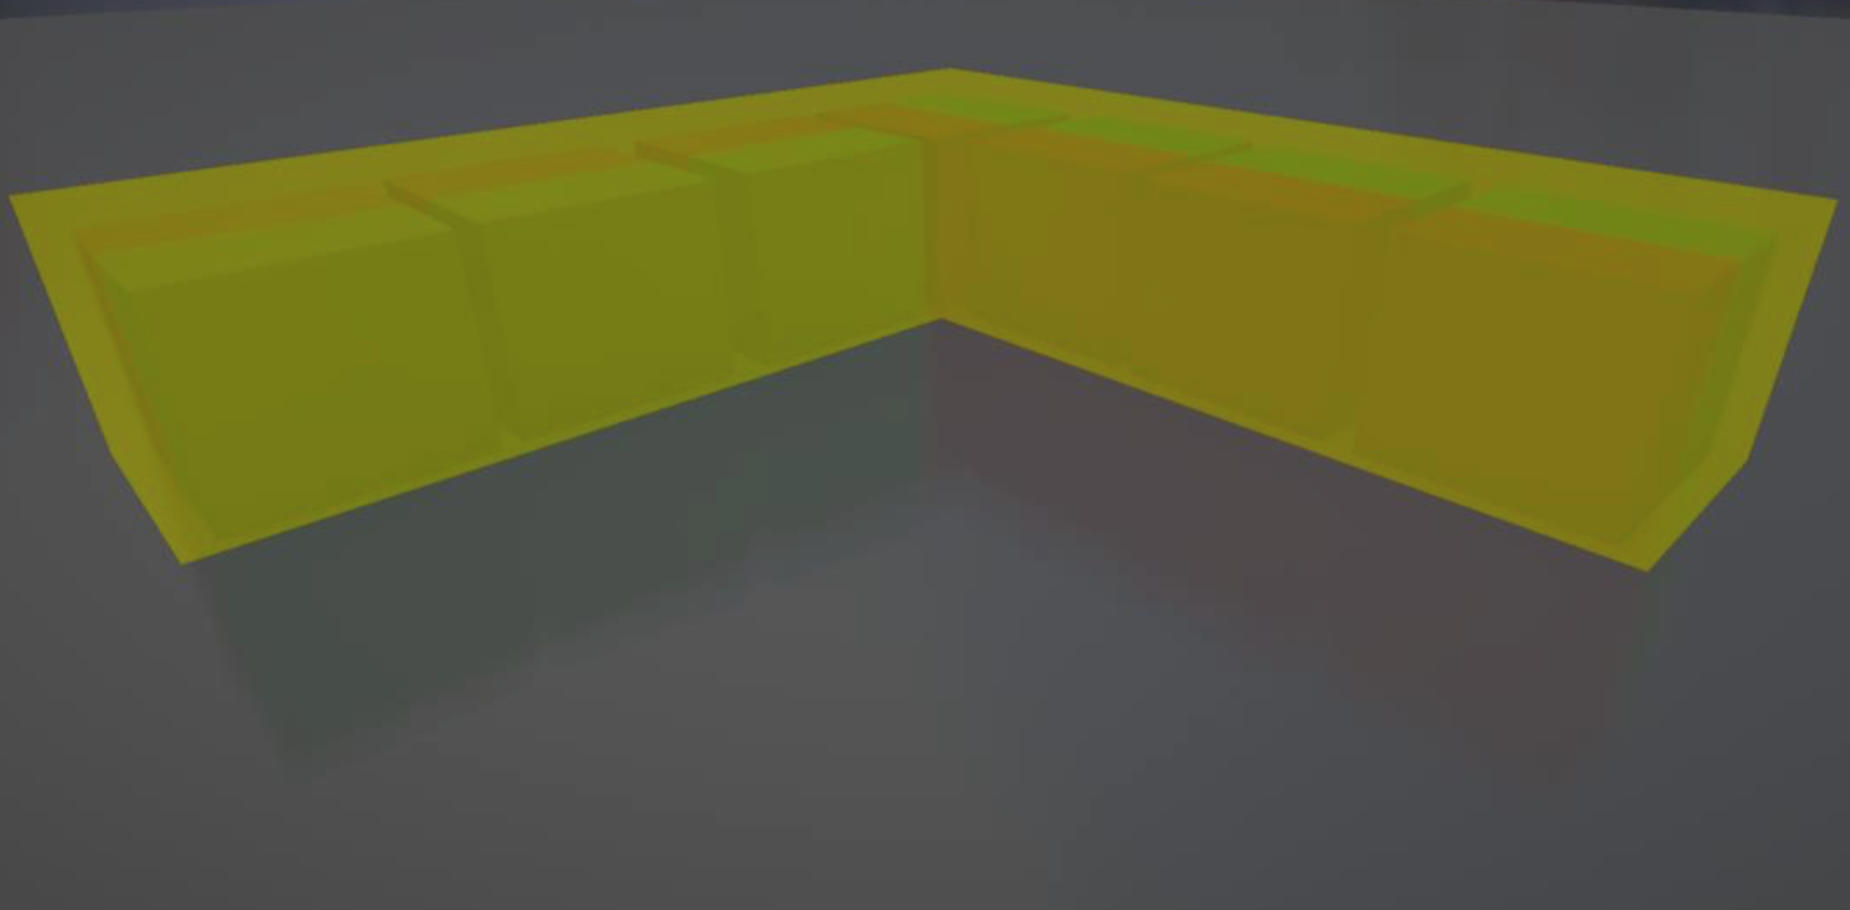
\includegraphics[width=\textwidth]{figures/vct/vct-11-4}
		\caption{各向同性混合的体素}
	\end{subfigure}
	\caption{一些具有不同颜色的盒子混合在一起,其中每个盒子填充一个体素,对这些体素的参数值进行过滤的最好的 方法就是分别对每个面进行计算,每次只对该面内的参数值计算平均计算,并对每个面单独存储一个独立的平均值参 数(图片来自\cite{a:TheTechnologyofTheTomorrowChildren})}
	\label{f:vct-11}
\end{fullwidth}
\end{figure}


理想情况下,我们希望能够精确地考虑预积分 $\overline{T}(\mathbf{p},\mathbf{d},s,l)$ 和 $\overline{Q}(\mathbf{p},\mathbf{d},s,l)$ 中的方向参数 $\mathbf{d}$,因为这样将使得,对于两个完全不透明体素的混合形成的子 体素,当从每个面观察该子体素时,它仍然是不透明的,而当从体素两个面之 间切向观察时,它们的值是半透明的,如图\ref{f:vct-5}右边小图所示。在图\ref{f:vct-11}中,我们希望当从红色的一面观察时,其混合后的体素参数值仍然是红色的,同样,当 从绿色一面观察时,其混合后的体素参数值仍然是绿色的,而当从这两个方向 之间观察时,其值才为这两种颜色值的混合。

\begin{figure}
\begin{fullwidth}
	\begin{subfigure}[b]{0.774\thewidth}
		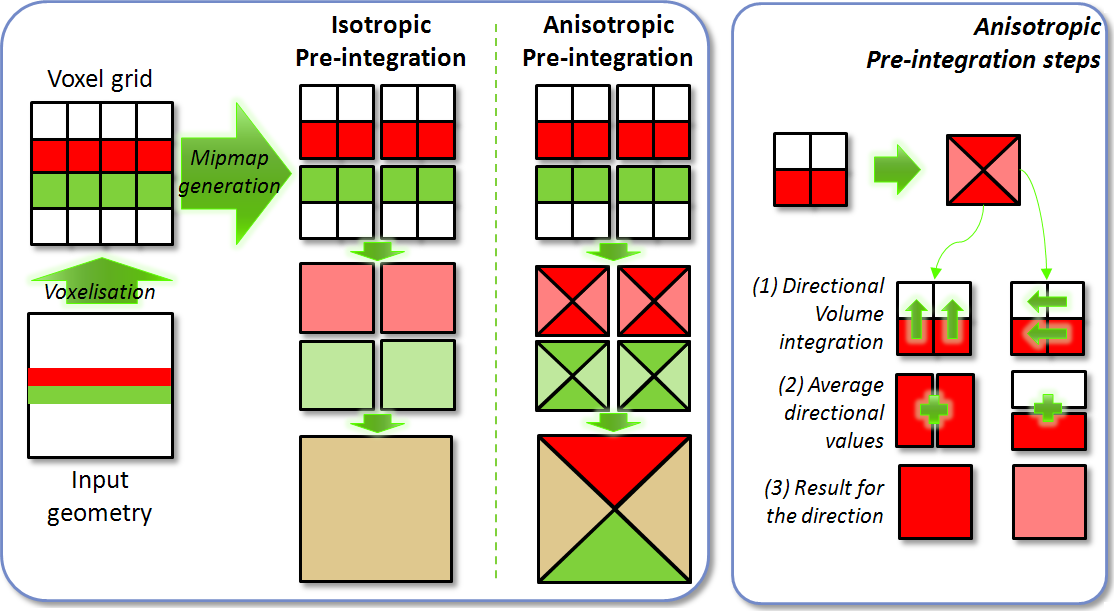
\includegraphics[width=\textwidth]{figures/vct/vct-5-1}
	\end{subfigure}
	\begin{subfigure}[b]{0.215\thewidth}
		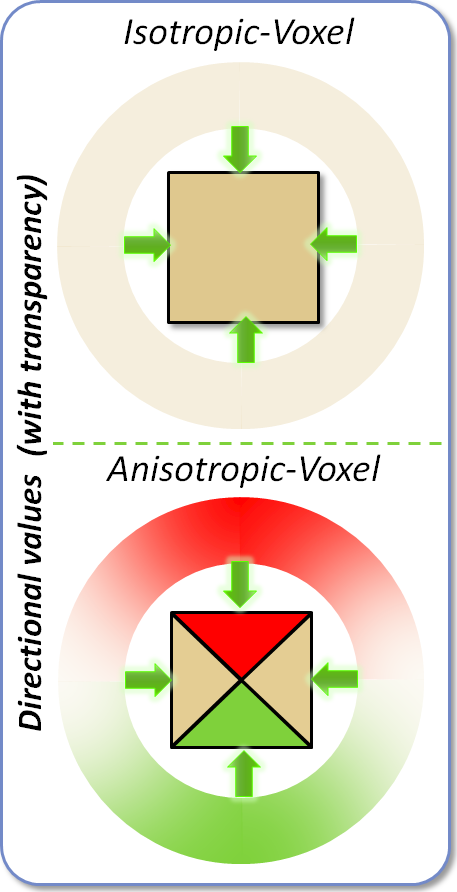
\includegraphics[width=\textwidth]{figures/vct/vct-5-2}
	\end{subfigure}
	\caption{左边矩形框内展示了多级体素的过滤使用各向同性(左)和各向异性(右)两种模型的过程和结果,中间的矩 形框内展示了方向积分的过程,右边的矩形框内展示了对体素的方向进行采样的结果分布(图片来自\cite{a:InteractiveIndirectIlluminationUsingVoxelConeTracing})}
	\label{f:vct-5}
\end{fullwidth}
\end{figure}

要精确地存储方向维度 $\mathbf{d}$ 中的每一个离散的方向,其成本是非常昂贵的,为 了实现这样的目标,这里使用了一个体素的各向异性表述,与上述各向同性模 型中对每个体素中每个参数仅存储一个值不同,这里选择对体素的 6 个面 分别存储一个参数值,其每个面代表了每个坐标轴上的两个方向,这样实 际上存储了 6 个离散的方向值。如图\ref{f:vct-5}所示,每个方向的参数值通过对体素 在该方向上的深度执行体积积分来计算, 然后对参数在这些方向上的积分结果 进行平均来计算下一级体素的参数值。最后在渲染的时候,每个方向上采样得 到的体素值,可以通过与该方向最相似的三个方向的体素值的线性插值计算出 来。

需要注意的是,这种方向性的表述仅需要对所有不是处于最高分辨率层级 的体素使用,即是说这些体素没有落于八叉树的叶节点上,一方面是因为存储 这种方向信息需要消耗大量的内存及其带来的带宽及读取延迟。因此,实际上 存储这些方向信息仅仅会导致 1.5 倍的内存占用。

图\ref{f:vct-12}展示了上述两种模型的渲染结果对比,可以看到各向异性模型能够 捕捉更多的细节信息。




\section{数据结构}\label{sec:vct-data-structure}
前面的内容假设已经存在一种多级体素结构,然后圆锥体追踪算法会直接 使用体素中的数据来计算光照贡献。然而,为了在 GPU 上实现高效的计算性 能,这个体素的数据结构并不是一个简单的金字塔结构,而是一个复杂的两种 结构的混合体,这样的结构既要能够节省内存,又能利用 GPU 的硬件特征,例 如三线性插值以及缓存特征。

理论上,最简单的方式就是直接将所有 3D 空间中的几何物体存储为一个 某种形式的多分辨率的体积结构,例如八叉树结构,这样该八叉树中的每一个 节点表示场景空间中的某个几何体积,同时存储着该体积对应的相关参数。然 而这会导致一些弊端,例如所有节点所占用的内存空间大小应该是相同的,即 是一种规则的结构,不然就很难对其进行过滤和节点的添加/删除管理,但是这 种规则的结构又会浪费大量的内存,因为大部分 3D 空间不包含任何表面,例 如那些空白区域和不透明物体内部所占据的区域。

在本章基于体素的全局光照技术中,这种关于多级体素的数据表述是其成 功以及能够实现高效实时计算的一个重要基础。\cite{a:Gigavoxels:Avoxelbasedrenderingpipelineforefficientexplorationoflargeanddetailedscenes}第一次提出了一种八叉树 + 纹理块的一种联合表述,这种数据结构的内存占用非常紧凑,并 且能够在渲染时提供非常快速的遍历操作,以及非常容易对节点进行修改和更 新等操作。以下我们首先讨论这种联合的数据结构,然后再讨论怎样对这个结构中的节点进行构造和动态更新。



\subsection{八叉树+块的联合表述}\label{sec:vct-block-plus-octree}
基于上面提到的问题,这里关于数据结构做的第一个选择就是将体素的空间结构与其所记录的参数数据分离开来,其中体素的空间结构存储在一个阶层 式的规则的八叉树(octree)\myindex{八叉树}{octree}中,该八叉树的每一个节点表示一个空间体积,但它并不是一个体素,其每个指向非空白区域和不透明物体内部区域的节点,都(通过指针)关联着一个低分辨率的块(brick)\myindex{块}{brick}结构,我们称这个块结构为我们最终需要的体素,该块结构存储在一些 3D 纹理中,这些小尺寸的 3D 纹理存储 着体素的参数数据,用于近似八叉树中对应节点对应体积内的表面。例如,对于八叉树根节点对应的块,它存储的数据可以近似整个场景内的表面,这样的联合结构如图\ref{f:vct-octree}所示。

\begin{figure}
	\sidecaption
	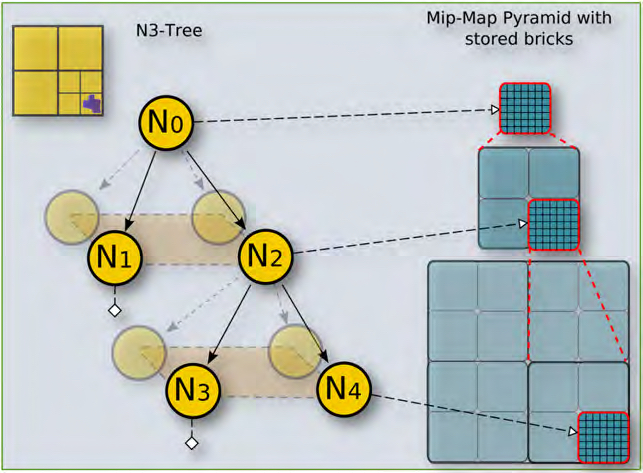
\includegraphics[width=0.65\textwidth]{figures/vct/vct-octree}
	\caption{稀疏的体素八叉 树结构,这个结构存储整个 场景以及其在多个分辨率上 预过滤的体素,其中每个八 叉树的节点关联一个块数 据,这个块数据存储为一个 3D 纹理,正式这种分离的 阶层式结构,使得可以使用 非常稀疏的空间存储整个场景(图片来自\cite{a:Gigavoxels:Avoxelbasedrenderingpipelineforefficientexplorationoflargeanddetailedscenes})}
	\label{f:vct-octree}
\end{figure}

这种联合的数据结构具有多方面的优点,首先八叉树结构使得存储非常紧凑,因为与体素数据分离,因此空白区域和物体内部区域可以直接存储为一个简单的常数值,而不需要关联一个块数据,对当前视图不可见的区域也可以完全忽略掉(这个优点是因为基于指针的结构形成的);其次,由于每个体素内的数据存储在一个小的 3D 纹理 中,因此对于一个体素内的任意位置,它的值可以通过图像硬件提供的线性插 值计算出来;最后,八叉树的每个节点和体素块的尺寸都是常数,因此很容易 对这些数据进行管理,例如动态更新。



\subsubsection{常数区域}
如后面的内容可知,八叉树的每个节点存储一个指针用于指向内存中一 个块的存储位置。但对于那些空白区域和物体内部的区域,存储一个块则是很浪费的,因此这些节点仅存储一个常数值,以代替用于引用块的指针 所占据的数据位,即这些数据位要么存储一个常数值,要么存储指向一个块的指针。

这种存储结构不仅能节省内存占用,而且在渲染的时候,我们可以直接停 止对这些常数区域以下的节点的遍历和对纹理数据的查询操作,而是直接使用 这些节点存储的常数值作为这些区域的贡献值。对于这些常数值,如果其所在 的区域是空白区域,则其值为 0,如果是内部区域,则其存储的是对其子节点 向下采样得到的过滤数据,这样这些数据可以被直接用于着色计算。



\subsubsection{体素块}
每个体素块与某个节点关联,该体素块中存储的数据是对该节点所占体积 内表面的一个近似,因此理论上,每个体素块(对于各向同性模型)只需要对 于前面介绍的每个参数存储一个值即可,或者说(在各向异性模型下)在每个离散的方向下分别存储这些参数值,这些参数包括平均漫反射颜色,平均法线 值,透明度等,然后在对体素采样时直接读取这些参数值即可。

然而,一个体素块代表的是一个很大的空间区域,因此也即是对应着很大 的表面区域,即使是对于八叉树的每个叶节点,它也要比一般的像素尺寸要大 得多,体素结构的分辨率是非常低的,我们用一个概率密度分布函数来近似一 个很大体积空间内的表面细节,例如法线分布函数,从而能够大大提升实时计 算的性能。因此,即使对于给定细节层次下的一个体素,光线可能落于该体素 对应空间的任何区域,这就需要我们能够在每个体素内执行插值计算。这也是 为什么体素样本的插值称为四线性插值,参见第\ref{sec:vct-quadrilinear}的内容,其中一个双线 性插值来源于体素内,也即是这里讨论的内容,而另一个双线性插值来源于体 素之间。

显然,如果仅对每个体素块存储单套(即对每个参数分别存储一个)像素 值,这样是无法在体素之间进行插值计算的,除非我们能够很巧妙的将所有纹 素组织在一个独立的 3D 纹理中,因为 GPU 的硬件特性是仅能够对一个纹理 执行线性插值计算,但是这在我们这里的结构中是不可行的,如前面的内容可知,为了保持存储的紧凑,八叉树节点本身是稀疏存储的,这意味着有很多节点在某些层级是没有对应的体素块的。

由于在空间上相邻的体素在纹理内存中可能并不是相邻的,因此要想对体 素在纹理空间执行线性插值,其唯一的方法就是允许一定的冗余,对于每个体 素块,它除了存储其对应节点的参数,还需要存储这个节点所有相邻节点的参 数数据,这样保证每个空间上相邻的体素,其纹理数据也是相邻并存储于同一 个纹理中的,因此纹理的线性插值特性可以被用上。

有两种方式可以实现这样的冗余结构,第一种称为拐角居中(corner-centered) \myindex{拐角居中}{corner-centered)}体素,即让体素的中心与节点的拐角重合,如图\ref{f:vct-13-11}所示;第二种称为节点居中(node-centered)\myindex{节点居中}{node-centered}体素,它让体素的中心与节点的中心重合。为了实现双线 性支持,在拐角居中结构中的体素是一种 $3\times  3\times  3$ 的体素结构,即每个体素存储 27 个体素数据,它们存储于一个 3D 纹理中,这些体素分别来自中心体素周 围相邻的 $2\times 2\times 2$ 个节点中,如图\ref{f:vct-13-11}所示。拐角居中的方法比节点居中的 方法要节约一半以下的存储占用。

\begin{figure}
	\sidecaption
	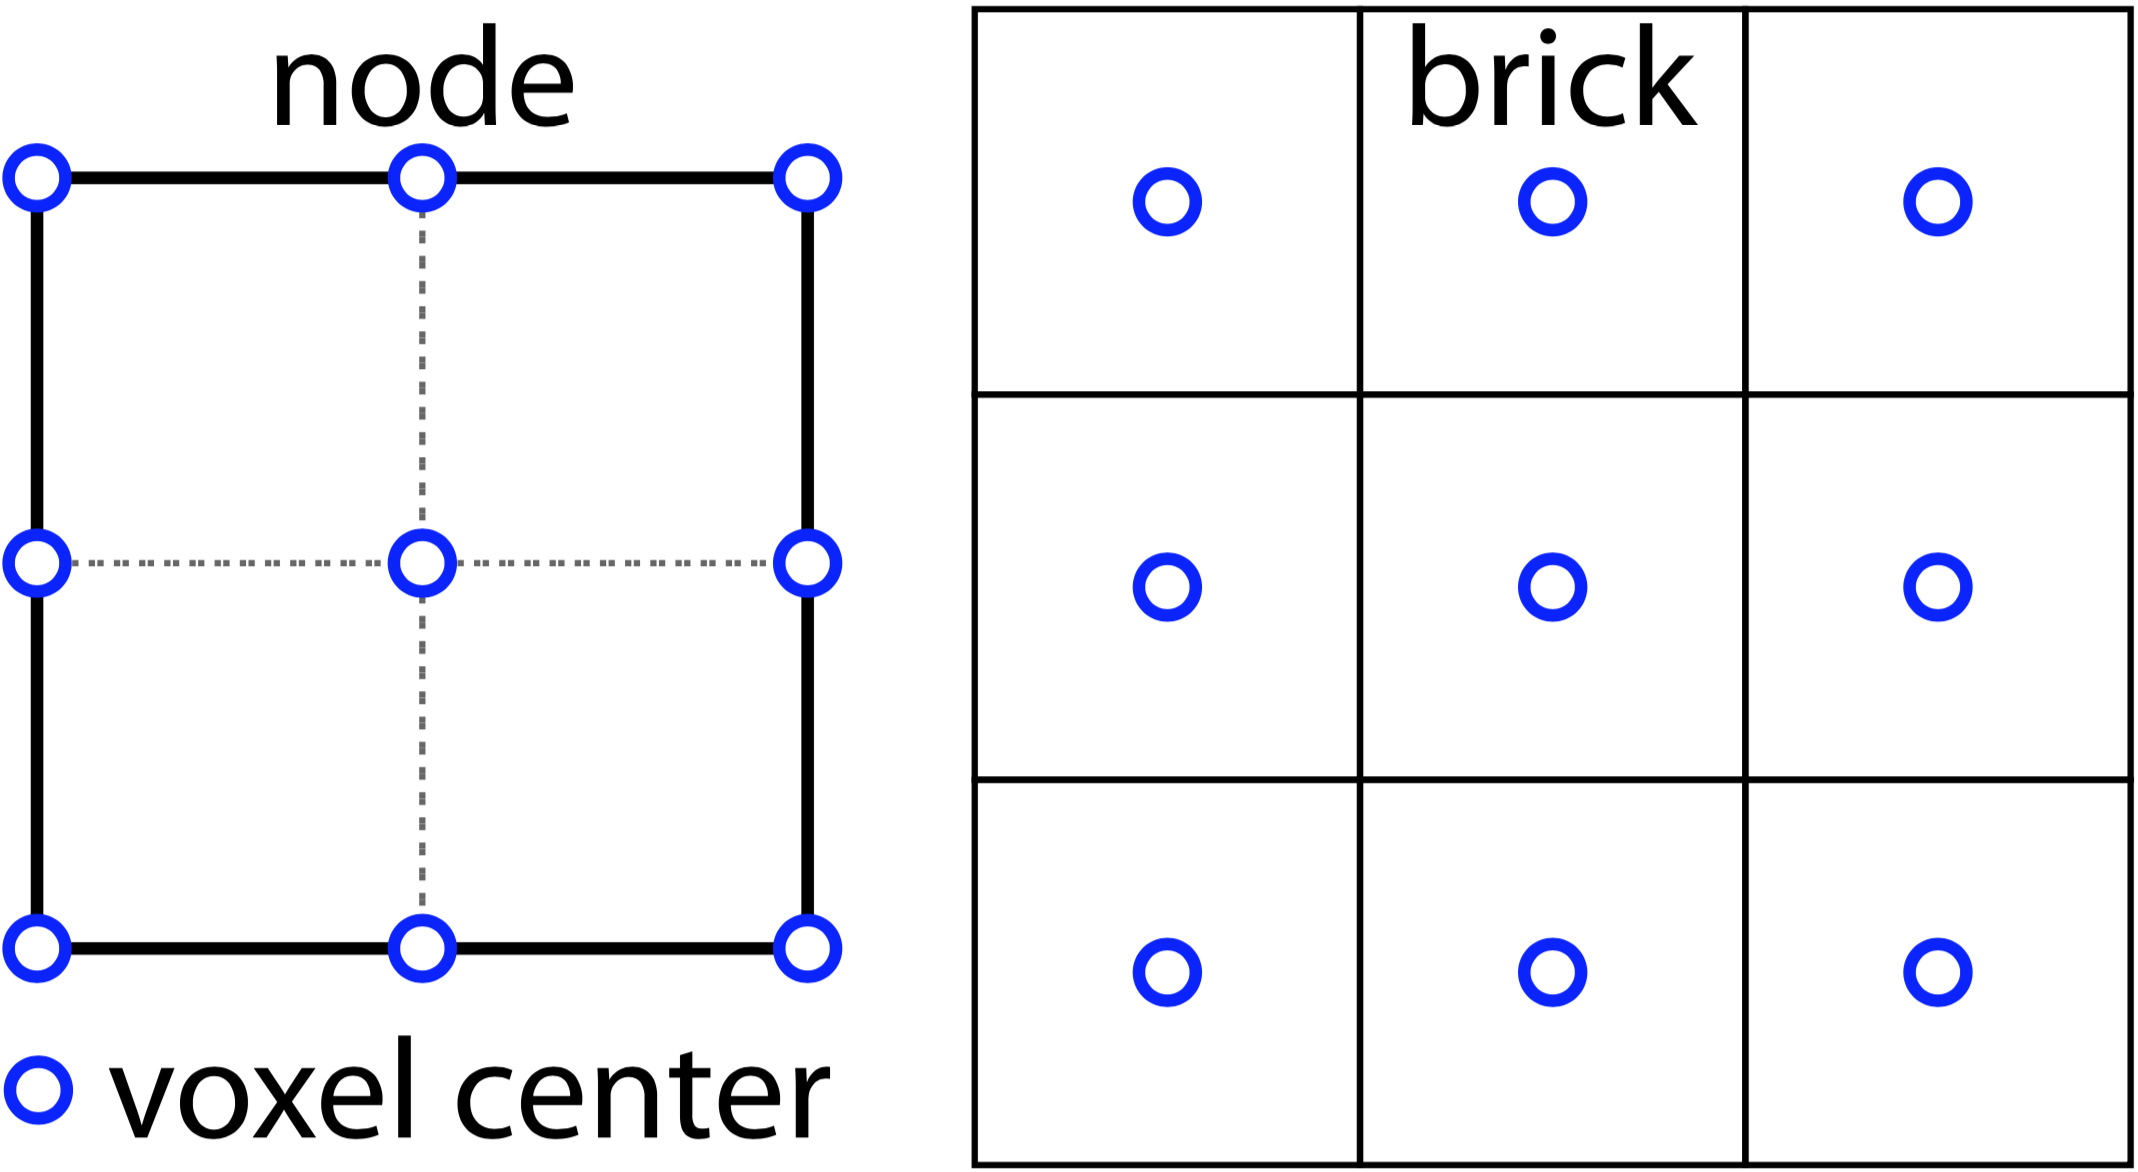
\includegraphics[width=0.45\textwidth]{figures/vct/vct-13-11}
	\caption{体素块(在2D平面上)的拐角居中表述方式,其中蓝色小圆点表示一 个体素块的中心,左图的正方形表示八叉树中的一个节点,右边的正方形表示一个 体素块}
	\label{f:vct-13-11}
\end{figure}



\paragraph{体素的预过滤}
当这样的八叉树结构被建立(参见后面第\ref{sec:vct-octree-build-and-update}节的内容)之后,所有的表 面材质参数被写入到八叉树的叶节点上,然后我们需要对这些参数值执行过滤 计算,以生产一个金字塔的多级体素结构。对于一个层级为 $n$ 的八叉树,这就是简单地执行 $n − 1$ 次迭代,其中在每一次迭代中,当前层级的每个次级节点 被分配一个线程,这个线程对前一级节点对应体素中的参数值执行平均计算。

尽管这个过程看起来非常简单,但是由于我们使用了拐角居中的体素块结 构,这使得过滤计算要稍微复杂一些。如图\ref{f:vct-13-11}所示,由于每个节点实际上存 储了一个 $3\times  3\times  3$ 结构的体素块,这些相邻节点对应的体素到该体素的中心具 有不同的距离,因此这些相邻体素的过滤计算应该被分配不同的权重系数,而 不是简单地(像节点居中方法中那样)对其执行平均值计算。实践中,这跟一 个 $3^{3}$ 的高斯核函数结果是类似的,在该核函数下,每个相邻体素对应的权重系 数如图\ref{f:vct-mipmapping}所示。

\begin{figure}
	\sidecaption
	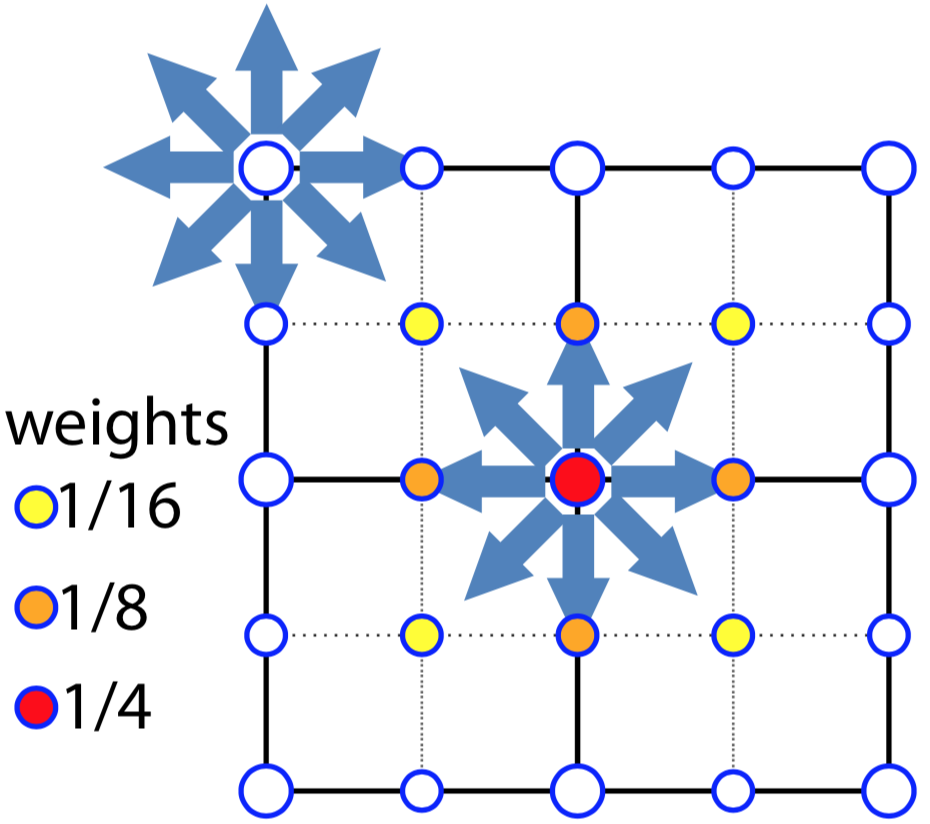
\includegraphics[width=0.42\textwidth]{figures/vct/vct-mipmapping}
	\caption{在拐角居中体素 块表述下,每个相邻体素距 离中心体素具有不同的距 离,因此不同的距离被分配 一个不同的权重系数}
	\label{f:vct-mipmapping}
\end{figure}

我们将在后面介绍怎么样将体素的参数值转移到相邻体素中去,以及怎样 以高效的方式对这种体素块结构执行过滤计算。



\subsubsection{基于指针的八叉树结构}
前面的内容已经将每个体素块统一为一个固定的尺寸,例如不管是对于八 叉树的根节点还是叶节点,其对应的体素块均包含固定的 $3\times  3\times  3$ 的体素值 结构,因此这些块可以在内存中以很规则的方式存储起来,这是保持存储紧凑 的一个重要条件,我们将在本节后面讨论这种存储所有体素块的规则内存结构, 在那里称为一个块池。

类似地,我们也希望八叉树中的每个节点也占据相同尺寸的存储空间,同时 还要能提供高效的遍历操作,例如要能充分利用内存的一致性。\cite{a:Gigavoxels:Avoxelbasedrenderingpipelineforefficientexplorationoflargeanddetailedscenes}提出了一种基于指针的八叉树结构,在这种结构中,每个父节点下的 $N^{3}$(这 里 $N = 2$,即标准的八叉树结构)个子节点在内存中被连续地存储一起,如 图\ref{f:vct-pools}(a)所示,这样每个父节点只需要一个指针就可以找到其所有子节点, 这只需要指定一个适当的偏移即可,这既节省了内存,同时也使子节点在内存 中的位置满足内存一致性,其它一般的八叉树结构则需要分别为每个子节点存 储一个指针;除此之外,每个节点还存储一个指针用于关联一个体素块,如果 该节点位于空白区域或者物体内部,则该指针空间存储为一个常数值,八叉树 每个节点的数据结构如图\ref{f:vct-node-texel}所示。

\begin{figure}
	\sidecaption
	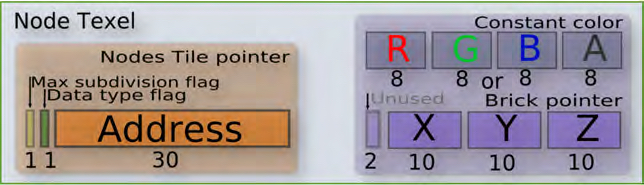
\includegraphics[width=0.65\textwidth]{figures/vct/vct-node-texel}
	\caption{八叉树每个节点 的数据结构,其包含一个指 向子节点的指针,以及一个 指向体素块的指针,如果该 节点处于常数区域,则体素 块指针转换为一个常数值}
	\label{f:vct-node-texel}
\end{figure}

在图\ref{f:vct-node-texel}所示的结构中,每个节点总共占据 $2\times 32$ 位,其中第一个 32 位 用于定义八叉树结构,另一个 32 位用于存储体素数据,其体素数据可能是一 个常数值或者一个指向体素块的指针。第一个 32 位包含两个指示位,其中第 1 位用于指示该节点是否在叶节点,第 2 位用于指示该节点的体素数据是一个常 数值还是一个指针。



\paragraph{内存池子}
八叉树的节点和体素块都存储为一种预分配(pre-allocated)\myindex{预分配}{pre-allocated}的称为内存池 (pools)\myindex{内存池 }{pools}的区域,这些池子的尺寸是在初始化时被固定的,\cite{a:Gigavoxels:Avoxelbasedrenderingpipelineforefficientexplorationoflargeanddetailedscenes}提供了 一种在 GPU 中以类似 CPU 缓存管理的机制管理这些内存池的机制,这里我们关注的重点是其全局光照的算法结构及原理,感兴趣的读者请自行前往阅读该论文第 7 章的内容。其中的节点内存池(node pool)\myindex{节点内存池}{node pool}用于存储八叉树的节点, 而块内存池(brick pool)\myindex{块内存池}{brick pool}用于存储体素块的数据,如图\ref{f:vct-pools}所示。

\begin{figure}
\begin{center}
	\begin{subfigure}[b]{0.4\textwidth}
		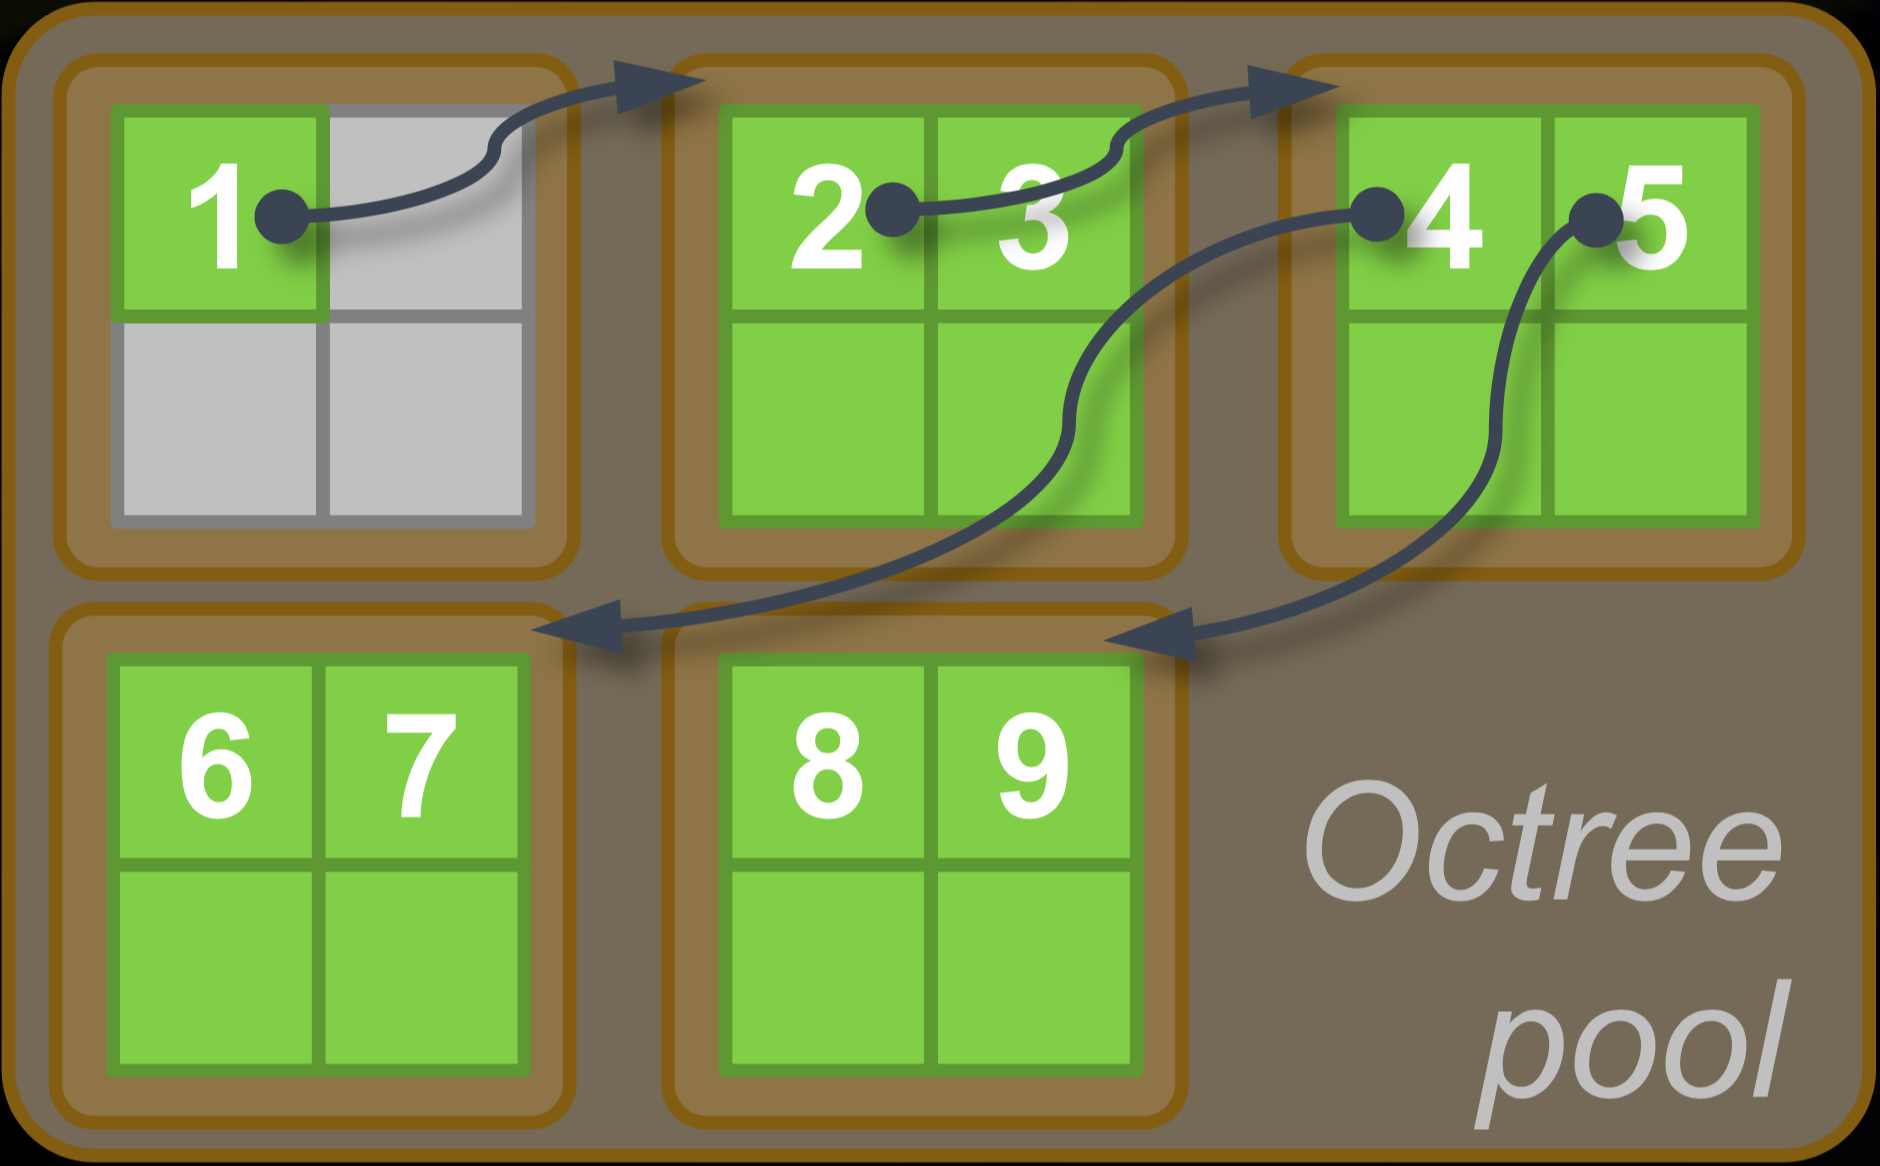
\includegraphics[width=\textwidth]{figures/vct/vct-13-8}
		\caption{Octree poll}
	\end{subfigure}
	\begin{subfigure}[b]{0.4\textwidth}
		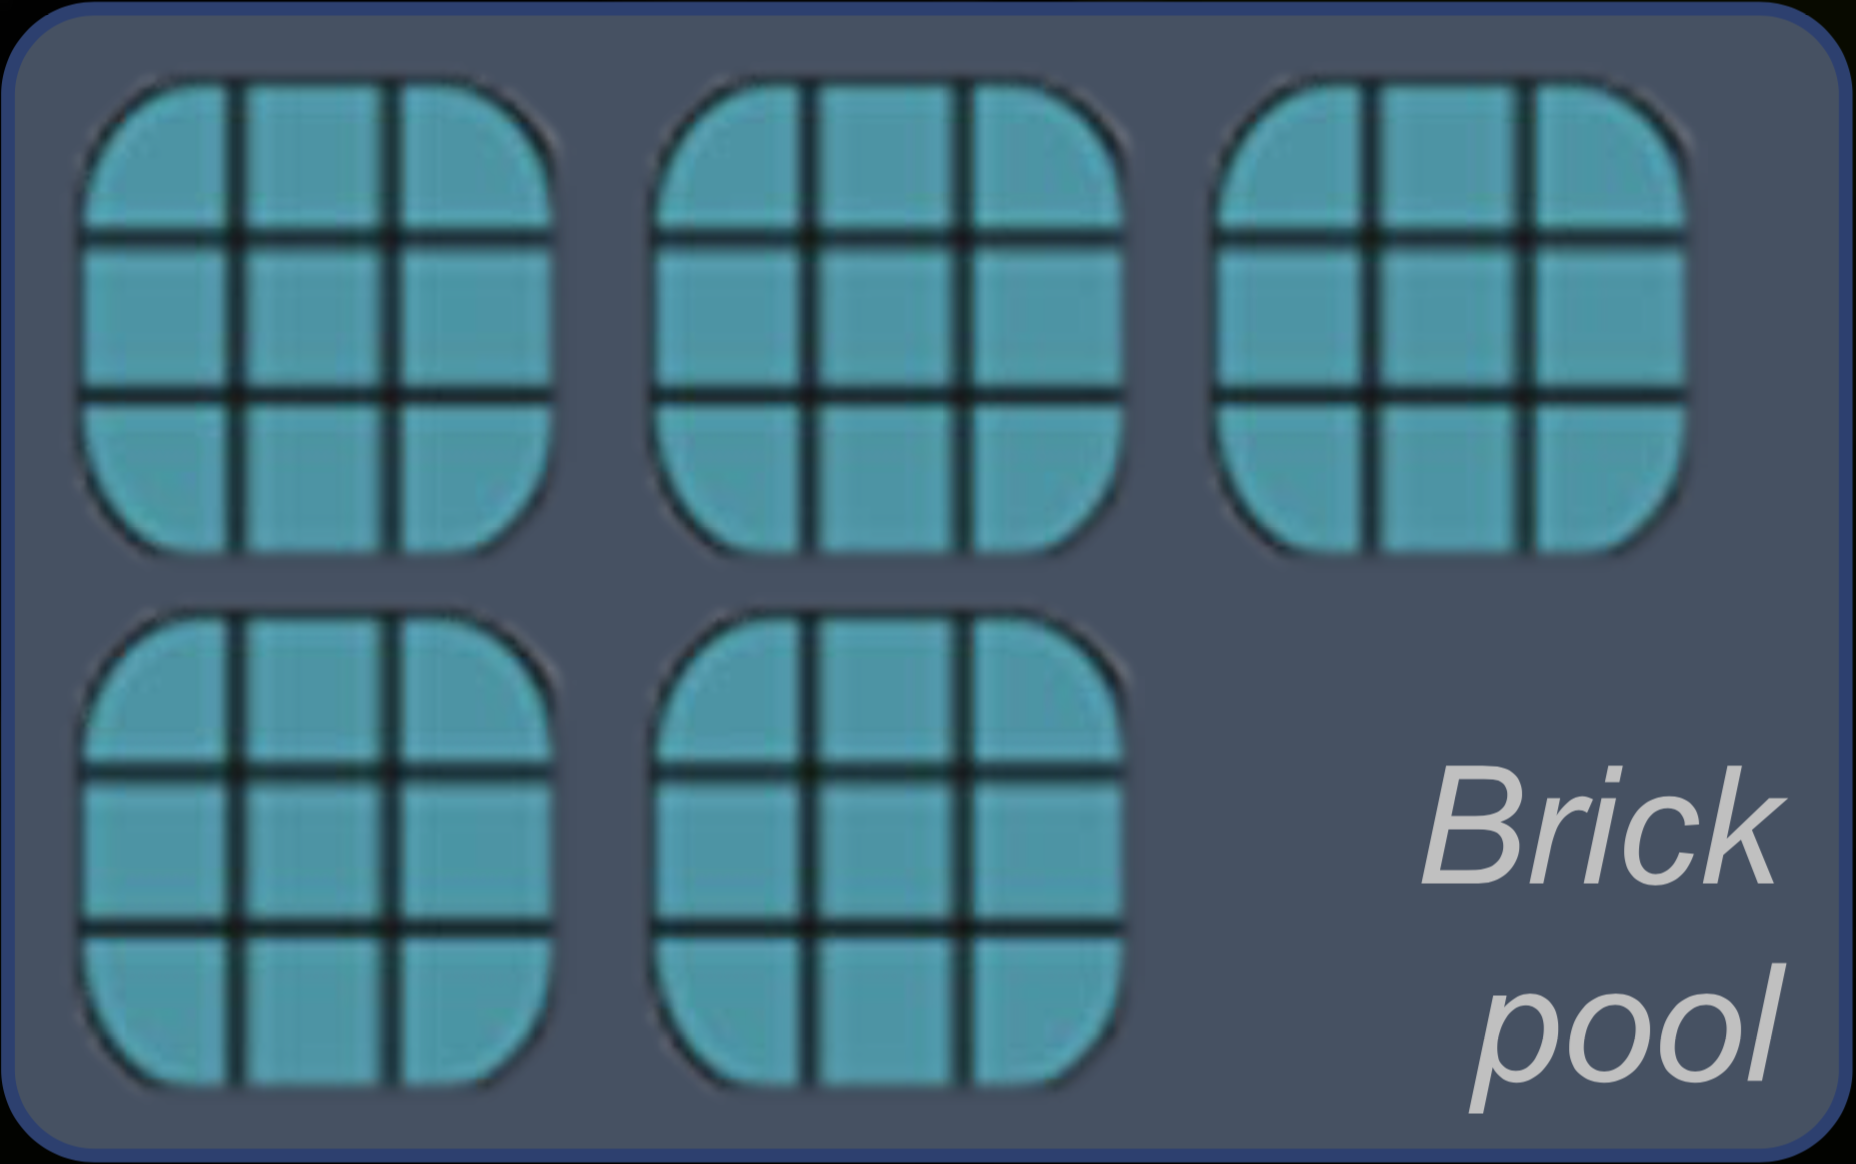
\includegraphics[width=\textwidth]{figures/vct/vct-13-9}
		\caption{Brick poll}
	\end{subfigure}
\end{center}
	\caption{规则的八叉树节点和体素块结构,其中体素块被存储于 3D 纹理中,它们表述了全 部分辨率下体素的近似,而八叉树的节点提供了体素的多级结构(图片来自\cite{a:Gigavoxels:Avoxelbasedrenderingpipelineforefficientexplorationoflargeanddetailedscenes})}
	\label{f:vct-pools}
\end{figure}

对于节点内存池,所有的节点都存储在一个线性的全局内存中,例如可能 是全局纹理内存或常量内存,这方面可以参见本书前面第$\ref{chp:hardware}$章的内容。为了提供 更好的缓存行为,节点内存中的每个连续的内存块实际上由具有共同父节点的 $N\times N\times N$ 个(这里 $N = 2$)子节点组成,而不是像传统方法一样将每个节 点独立存储,我们称这些 $2\times 2\times 2$ 个节点组成一个节点片(node tile)\myindex{节点片}{node tile},如 图\ref{f:vct-pools}左图所示。此外,为了使后面会讨论的遍历算法更加高效,节点数据中 的每一部分,即图\ref{f:vct-node-texel}中的节点描述和体素数据被分别存储在一个独立的数组 中,这种结构也称为数组结构(structure of arrays,SOA)\myindex{数组结构}{structure of arrays},这是因为实际上在渲染算法中这两部分通常不会交叉,这样的结构能够提升数据访问合并(data access coalescing)和纹理缓存效率。

体素块存储于 3D 纹理当中,这样能够充分利用图形硬件的纹理线性插值, 纹理空间 3D 位置寻址,3D 局部空间的缓存优化等特性。如前面的内容可知, 每个体素块同时存储周围 $2\times 2\times 2$ 个体素相关的 $3\times 3\times 3$ 个体素参数值,如 图\ref{f:vct-pools}(b)所示。此外,如前面的内容可知,体素可能存储单套(对于各向同性模型)或者多套(对于各向异性模型)参数值,对于后者,每个离散方向的 参数值存储于纹理的一个不同的层级(layer)中。




\subsection{八叉树构造与更新}\label{sec:vct-octree-build-and-update}
在渲染的时候,本节介绍的多级体素结构会完全代替原本的几何网格基元 数据,被用于执行光照计算。并且这样的体素结构会使得渲染中的插值和过滤 计算变得非常简单。

本章介绍的基于体素的全局光照算法是一种完全动态的方法,因此上述的 多级体素结构需要能够被快速的构建和更新。为了能够快速地将任意复杂度的 基于三角网格的场景转化为上述的多级体素结构,\cite{a:Gigavoxels:Avoxelbasedrenderingpipelineforefficientexplorationoflargeanddetailedscenes} 提出了一种 基于 GPU 光栅化管线的场景体素化方法,这种方法能够快速地构建上述的体 素结构,并对这些体素内存储的参数值执行过滤计算。

考虑到在大多数情况下,场景中的大部分场景是静态的,或者只是随着用 户的交互发生局部更新,因此这些物体的体素一旦被构建之后可以在内存中保 存起来,直到需要的时候再对其进行更新,而只有那些完全动态的物体才需要 每一帧都对其进行更新。

为了保持一个统一的遍历和过滤算法,这里将所有半静态和完全动态的物 体都存储一个八叉树结构中,为了区分两种类型的节点,这里使用一个时间戳 以阻止半静态的物体被频繁地更新。

\begin{myshaded}
	如果对渲染的概念及各种模型足够熟悉,这里可能会产生这样一个疑问,可见性 是关于物体之间的遮挡,而我们的体素参数中是包含可见性信息的,那么将动态物 体进行单独更新是否合适,例如它们被那些没有被更新的静态物体遮挡怎么办?即 理论上我们是无法独立地仅体素化场景中的一部分(例如动态的部分)的。
	
	回答这个问题的关键是,本章的模型将物体之间的遮挡转化为了一种近似的体积渲染的模型, 这种物体之间的相关性转化为了每个体素自身的一个属性,即不透明度,这个透明 度最后通过混合的方式形成一种对某条光线上可见性的近似,因此可见性信息被独 立出来,这样便能够通过独立地计算各个独立的部分,便可以编码可见性信息。基于 体积渲染积分的概念是本章基于体素的全局光照技术的核心,读者要仔细理解这种 概念及其形成的渲染模型。
\end{myshaded}



\subsubsection{八叉树构造}
为了高效地构建八叉树结构,这里利用了 GPU 的光栅化管线,我们对整 个网格场景执行三次光栅化渲染,分别沿着世界坐标系的三个主坐标轴,其中 的光栅化分辨率为八叉树最深层级对应的分辨率,例如对于叶节点为 $512^{3}$ 的八 叉树,其光栅化分辨率为 $512\times  512$,这样每个可能的叶节点都可以拥有像素着色 器中的一个线程,每个线程从上至下遍历八叉树,如果当前八叉树不存在像素 着色器处理的几何表面,则直接对八叉树执行进一步的细分。一旦叶节点被构 建,则将该像素着色器线程处理的几何表面的表面属性写入到体素中,由前面 的内容可知,这包括漫反射颜色,法线,以及表面的可见性。在光栅化管线中, 我们需要禁掉深度测试,因为这需要对所有物体执行体素化。

但是即使对于八叉树的叶节点,其粒度仍然是非常大,而每个体素实际上 只被分配了一个像素着色器线程,这要怎样计算体素内材质参数的平均值呢? 这里以不透明度为例进行分析,如图\ref{f:vct-voxel-1}所示,在一个像素着色器线程内,我 们可以对体素内的表面执行类似 MSAA 的超采样方法\cite{a:Practicalreal-timevoxelbasedglobalilluminationforcurrentgpus},这得 到一些分辨率更小的像素点,然后将这些超采样点投影到体素的某个面上,由 于这些离散采样仍然可能存在较大的方差,所以最后我们需要对这些采样结果 执行过滤使其更加平滑。在这个超采样过程中,法线和漫反射颜色平均值也可 以一并被计算出来。

\begin{figure}
\begin{fullwidth}
	\begin{subfigure}[b]{0.2425\thewidth}
		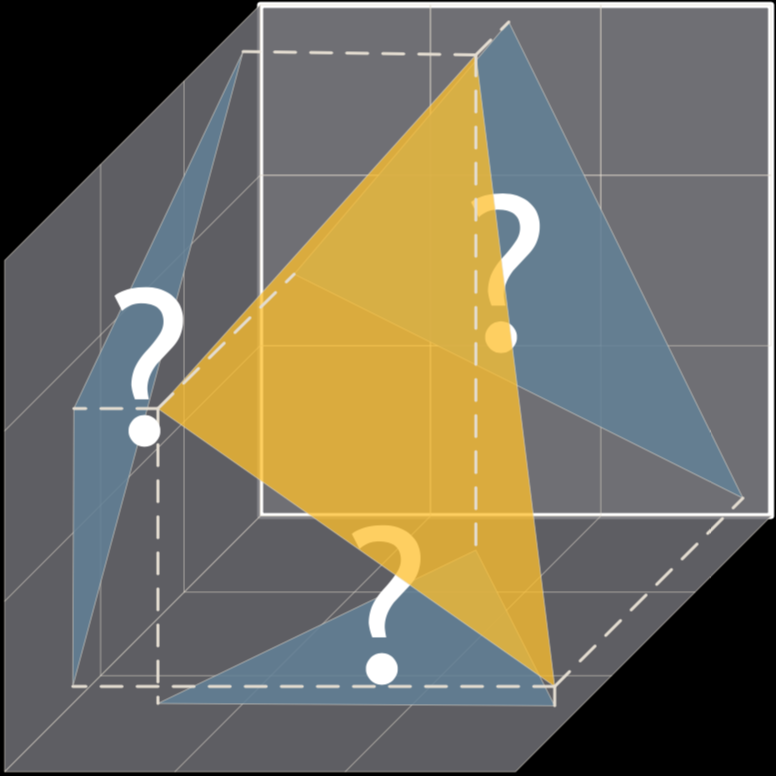
\includegraphics[width=\textwidth]{figures/vct/vct-voxel-1}
		\caption{光栅化}
	\end{subfigure}
	\begin{subfigure}[b]{0.2425\thewidth}
		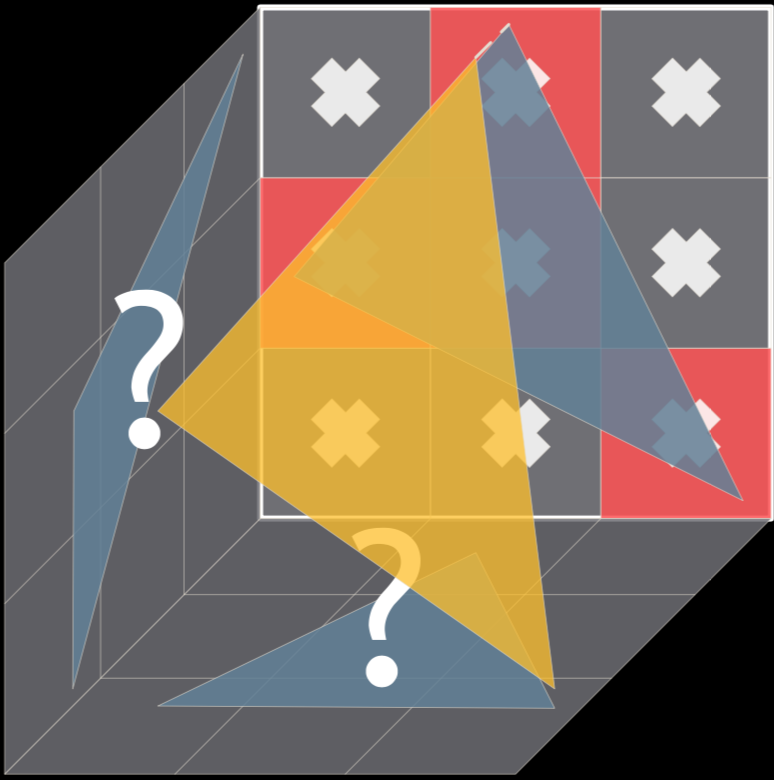
\includegraphics[width=\textwidth]{figures/vct/vct-voxel-2}
		\caption{MSAA超采样}
	\end{subfigure}
	\begin{subfigure}[b]{0.2425\thewidth}
		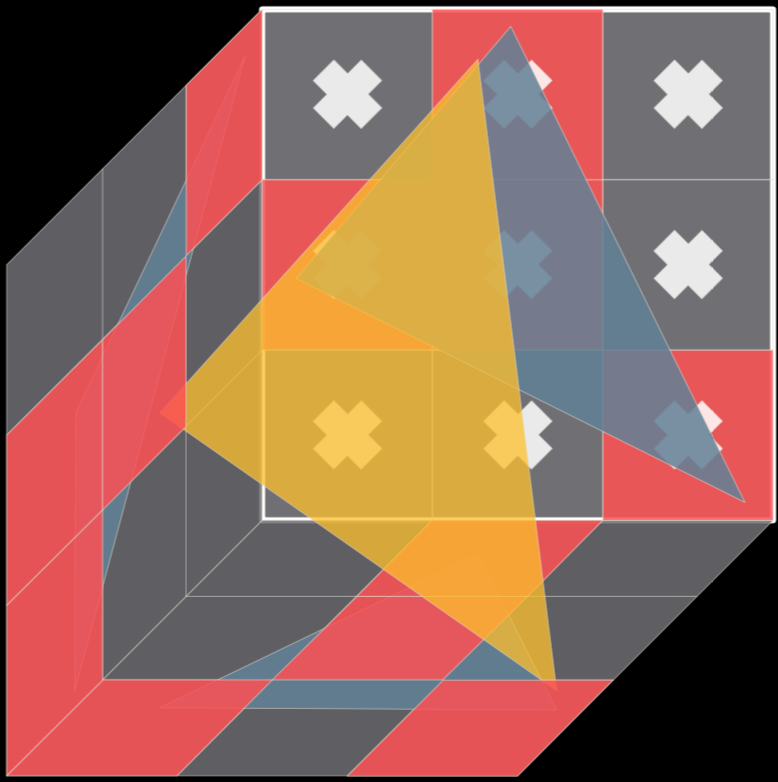
\includegraphics[width=\textwidth]{figures/vct/vct-voxel-3}
		\caption{三个面超采样}
	\end{subfigure}
	\begin{subfigure}[b]{0.2425\thewidth}
		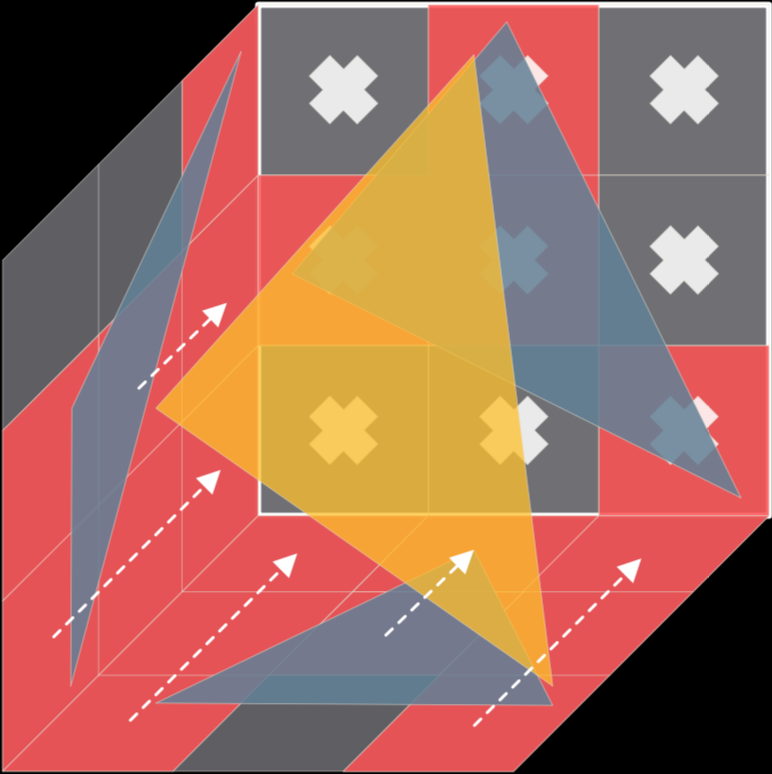
\includegraphics[width=\textwidth]{figures/vct/vct-voxel-4}
		\caption{过滤}
	\end{subfigure}
	\caption{八叉树结构通过使用光栅化管线进行渲染构建,其中每个叶节点被分配一个像素着色器线程,在每个体素内, 使用类似 MSAA 的超采样技术对表面进行采样,并将这些数据写入到体素中(图片来自\cite{a:Practicalreal-timevoxelbasedglobalilluminationforcurrentgpus})}
	\label{f:vct-voxel-1}
\end{fullwidth}
\end{figure}

当八叉树的一个节点需要被进一步细分的时候,节点内存中一块连续的 内存被分配,这块内存需要刚好能存储整个 $2\times 2\times 2$ 子节点,这块内存的地址被写入到父节点的第一个指针中去,然后线程继续向下迭代,直至叶节点被构 建。这里的分配需要使用原子增量(atomic increment)\myindex{原子增量}{atomic increment}的方式,它告诉我们共 享内存中下一个可用的节点位置。

由于多个线程可能会同时对一个节点执行细分操作,因为每个线程都是从 上至下迭代,例如在深度上重合的两个线程都可能同时对一个节点执行细分请 求,因此这里需要对每个节点使用一个互斥锁,以确保细分请求始终只被第一 个线程执行。然而在 GPU 中,我们并没有一种简单的机制让其它线程进入休 眠等待状态。为了避免这种等待,这里实现了一个全局线程列表(global thread list)\myindex{全局线程列表}{global thread list},然后所有被打断的线程都放入到这个线程列表,这些线程将被稍后执行, 在每一个光栅化通道结束之后,这些全局线程列表中被延迟的线程再被重新执 行,这个时候由于不再需要光栅化的过程,因此使用一个简单的顶点着色器即 可。这样的延迟通道又可能会产生新的等待线程需要延迟执行,这样的过程重 复执行直到全局线程列表中的线程为空。



\subsubsection{动态更新}
八叉树中动态物体的更新仍然使用上述的光栅化流程,这些物体每一帧都 需要被执行光栅化,其区别是这些动态物体的更新不会覆盖八叉树中静态物体 部分,因此这些动态物体通常被放置于全局缓存的尾端。



\subsection{其它表述}
上述介绍的基于稀疏八叉树的数据结构\cite{a:InteractiveIndirectIlluminationUsingVoxelConeTracing}尽管比较紧 凑,但是其缺点是八叉树中存在太多指针,而指针是非常不适合 GPU 的计算 的,因为 GPU 并没有如 CPU 中那样的缓存系统,这种指针的任意跳转会加 大数据读取的延迟,所以 \cite{a:Gigavoxels:Avoxelbasedrenderingpipelineforefficientexplorationoflargeanddetailedscenes} 在 GPU 中根据算法的遍历和渲染特 征,实现一个类似 CPU 缓存机制的缓存管理机制,来弥补这种在 GPU 中使 用指针的缺陷。然而,在理想情况下,我们仍然希望能够在 GPU 中尽可能少 地使用指针,让指令读取的数据尽可能地连贯,以加速并行计算。

所以基于此考虑,\cite{a:TheTechnologyofTheTomorrowChildren}使用了另一种数据结构来存储体素,在 这里,每个分辨率下的所有体素被存储于一个完整的纹理中,这称为一个体素纹理(voxel texture)\myindex{体素纹理}{voxel texture},它跟普通的 3D 纹理没有什么区别,只不过其纹素存 储的是一个体素内的参数值,这和本章前面介绍的体素块中每个纹素的值是一 样的,唯一不同的是这里的整个场景的体素参数都存储在一个纹理中,即那些 在空间中连续的体素在纹理中也是连续的,不存在像前面的表述那样形成一些 $3\times  3\times  3$ 的小纹理块,并且也不存在需要复制边界纹理以便于利用 GPU 的线 性插值特性。

每个体素纹理内体素的分辨率是一样的,为了实现多分辨率的体素结构, 这里在空间中相同的区域形成多个交叉的不同分辨率的体素纹理,形成一个纹理阶梯(texture cascade)\myindex{纹理阶梯}{texture cascade},如图\ref{f:vct-texture-cascaded}所示。这种多分辨率的结构仍然能够提 供圆锥体追踪需要的细节层次,并且这些体素纹理可以根据当前视图位置,仅 对可见范围内的空间生成体素纹理。

\begin{figure}
	\sidecaption
	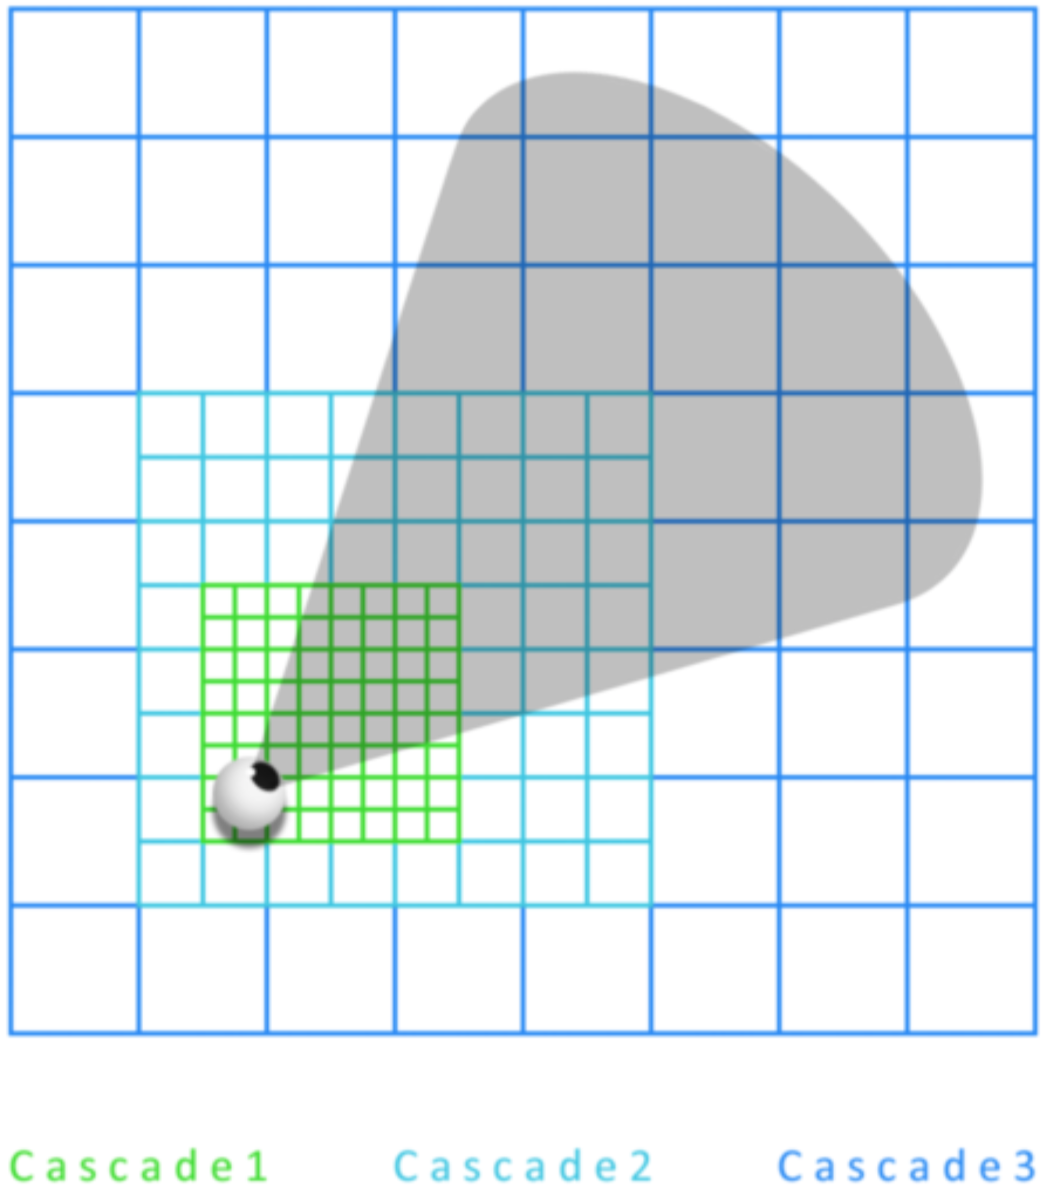
\includegraphics[width=0.45\textwidth]{figures/vct/texture-cascaded}
	\caption{以纹理阶梯的形 式表述多级体素结构,其中 整个场景的体素被存储在多 个不同分辨率的纹理中,形 成一个阶梯结构,通常我们 能根据当前视图位置调整体 素纹理所包含的空间}
	\label{f:vct-texture-cascaded}
\end{figure}




\section{渲~~染}\label{sec:vct-rendering}
我们已经了解了圆锥体追踪的基本思路,基于多级体素的全局光照算法的 原理,即使用体积渲染积分的思路来体素化场景,然后我们介绍了不同的构建 和存储这种多分辨率的体素结构的方法,最后本节将所有这些内容串联起来, 我们将讨论基于体素的全局光照算法的整体渲染逻辑。

在阅读本节之前,读者需要稍微留意的是,基于体素的全局光照技术大概 需要两个阶段,第一个阶段是构建体素表述及(在该构建过程中)对表面参数 的过滤,如上一节的内容所述;第二个阶段就是本节会讨论的渲染阶段。因此, 在本节内容的背景下,体素结构已经存在。实际上,我们认为第一个阶段的目 的主要是将用三角网格基元表述的几何场景,转化为一种使用体素作为基元表述 的几何场景,尽管这种新的基元形式是实时构建,而不是如网格场景在设计阶 段定制而成。我们可以认为基于体素的全局光照算法是一种对某种特殊格式的 基元表述(即多分辨率的体素结构)的渲染方法,当然这里的体素不是一般的 3D 数据,而是需要包含本章前面介绍的那些参数的 3D 体素,例如漫反射颜色 值,法线分布函数以及透明度。

我们可以将整个渲染过程分为三个步骤,如图\ref{f:vct-steps}所示,即:

\begin{figure}
\begin{fullwidth}
	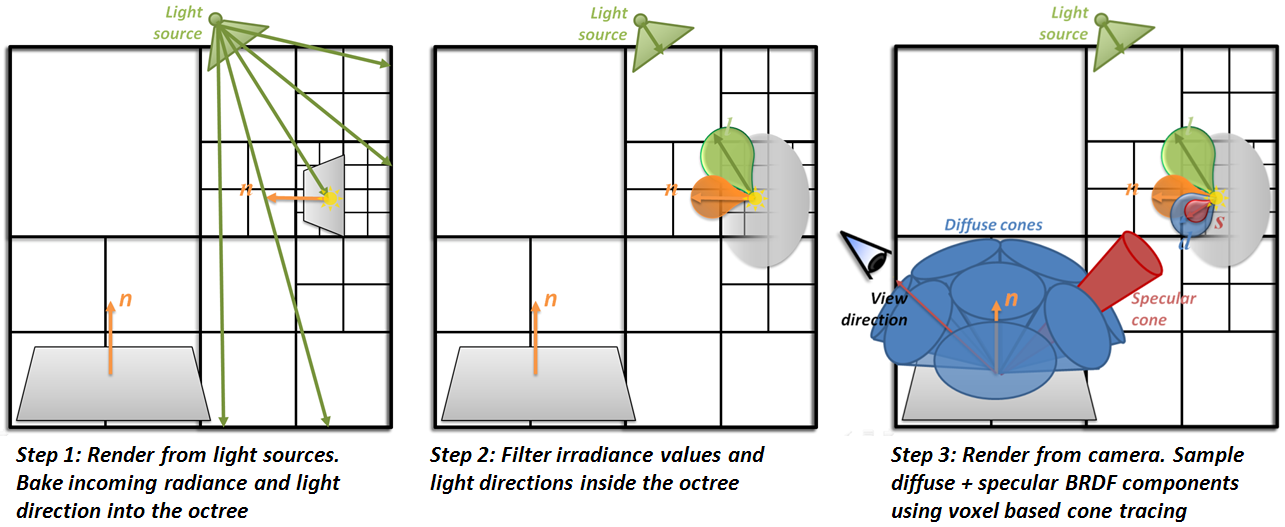
\includegraphics[width=\thewidth]{figures/vct/vct-3}
	\caption{基于体素的全局光照技术的三个基本流程及算法步骤,此时场景已经被转化为多分辨率体素的形式,在体素 预积分模型中,我们还需要实时地把入射光照信息注入到体素的叶节点,并过滤到各个分辨率下的节点中去,最后就 可以利用基于圆锥体追踪的方法计算来自体素的光照贡献(图片来自\cite{a:InteractiveIndirectIlluminationUsingVoxelConeTracing})}
	\label{f:vct-steps}
\end{fullwidth}
\end{figure}

\begin{itemize}
	\item 首先,我们将动态光源的入射能量(包括能量和方向信息)注入到稀疏八叉 树的各个叶节点上,这些能量即是前面介绍的预积分能量积分中的入射光照部分,这些能量最后与实时计算的体素 BRDF 函数一起积分计算出最终的 体素光照贡献。这一步可以通过从每个光源处执行一次光栅化渲染,在每个 像素着色器中将光源的光子撒向其表面所在的叶节点。
	\item 然后,我们对叶节点上的入射能量执行过滤,并将其值存储在八叉树中更高 一级(即更低分辨率)的非叶结点中,由于入射光照具有方向信息,所以这里 可以使用高斯函数来进行近似,本章前面已经介绍过两个高斯函数的过滤。
	\item 最后,我们从摄像机渲染整个场景,对于每一个可见的表面像素,它发射出 一条(或多条)光线,根据前面介绍的近似圆锥体追踪方法计算来自体素样 本中的光照贡献。
\end{itemize}

在冯氏 BRDF 模型中,通常使用少数几个(约 5 个)半径比较大的圆锥体就可以很好地近似场景的漫反射光照,对于光泽反射,则需要使用一个半径比较小的圆锥体,这个圆锥体的半径可以通过光泽表面的粗糙度参数推导出 来,这使得本章的模型可以很好地处理光泽反射。

以下我们首先简要总结一下对体素执行圆锥体追踪的基本思路和过程,然 后介绍怎样使用这种圆锥体追踪算法计算表面的环境遮挡以及间接光照。




\subsection{近似的圆锥体追踪}
本章前面的内容其实已经介绍了比较多的关于圆锥体追踪的概念,例如 第\ref{sec:vct-ray-tracing-in-a-cone}节介绍了圆锥体追踪的动机和工作原理,而第\ref{sec:vct-pre-integration-based-cone-tracing}节介绍了圆锥体追 踪能够实现的理论基础,即基于体积渲染积分的概念,将基于表面点样本的积 分转换为基于体积样本的积分。本节我们再对其进行简要的总结。

全局光照通常要求对场景执行很多光线采样,这个计算过程的成本通常很 高。在这些光线中,其中的一些光线具有非常好的连贯性,例如那些摄像机发出 的光线,一些算法充分利用了这种方向和空间上的连贯性,使得光线采样的计 算效率得到一定的提升,例如本书前面介绍的光线包(ray packets)\myindex{光线包}{ray packets}技术\cite{a:InteractiveRenderingwithCoherentRayTracing}等,相关的更多内容可以参见第\ref{sec:coherent-ray-tracing}节。

类似地,为了利用这种连贯性,\cite{a:RayTracingwithCones}基于对反走样执行过 滤的思路,提出了圆锥体追踪(cone tracing)\myindex{圆锥体追踪}{cone tracing}的方法和概念。

原始的圆锥体追踪技术非常复杂且计算成本很高,\cite{a:Gigavoxels:Avoxelbasedrenderingpipelineforefficientexplorationoflargeanddetailedscenes}引 入了一种预过滤的体素结构来同时地(parallel)近似一个光束(bundle)内多 条光线的计算结果。这种方法通过在圆锥体的主轴上步进,并在步进的过程中 从一个多分辨率的体素表述中对体素进行采样来计算体素的光照,其中每次步 进选择的体素样本的分辨率符合该采样位置处圆锥体的半径大小,如图\ref{f:vct-cone-tracing}所 示。对体素的采样使用四线性插值(参见第\ref{sec:vct-quadrilinear}节)来保证计算的结果不会发生走样,其中的一个双线性插值来源于每个层级内3D空间位置上的插值,因为光线步进 对体素的采样位置其实并不位于体素的中心,它需要对这些离散的体素值(在 3D 空间内)执行双线性插值;第二个双线性插值则用来对两个分辨率的体素采样结果执行插值计算,这原本是一个指数的关系,但是出于效率,仍然使用一个双线性插值来对其进行近似。

\begin{figure}
	\sidecaption
	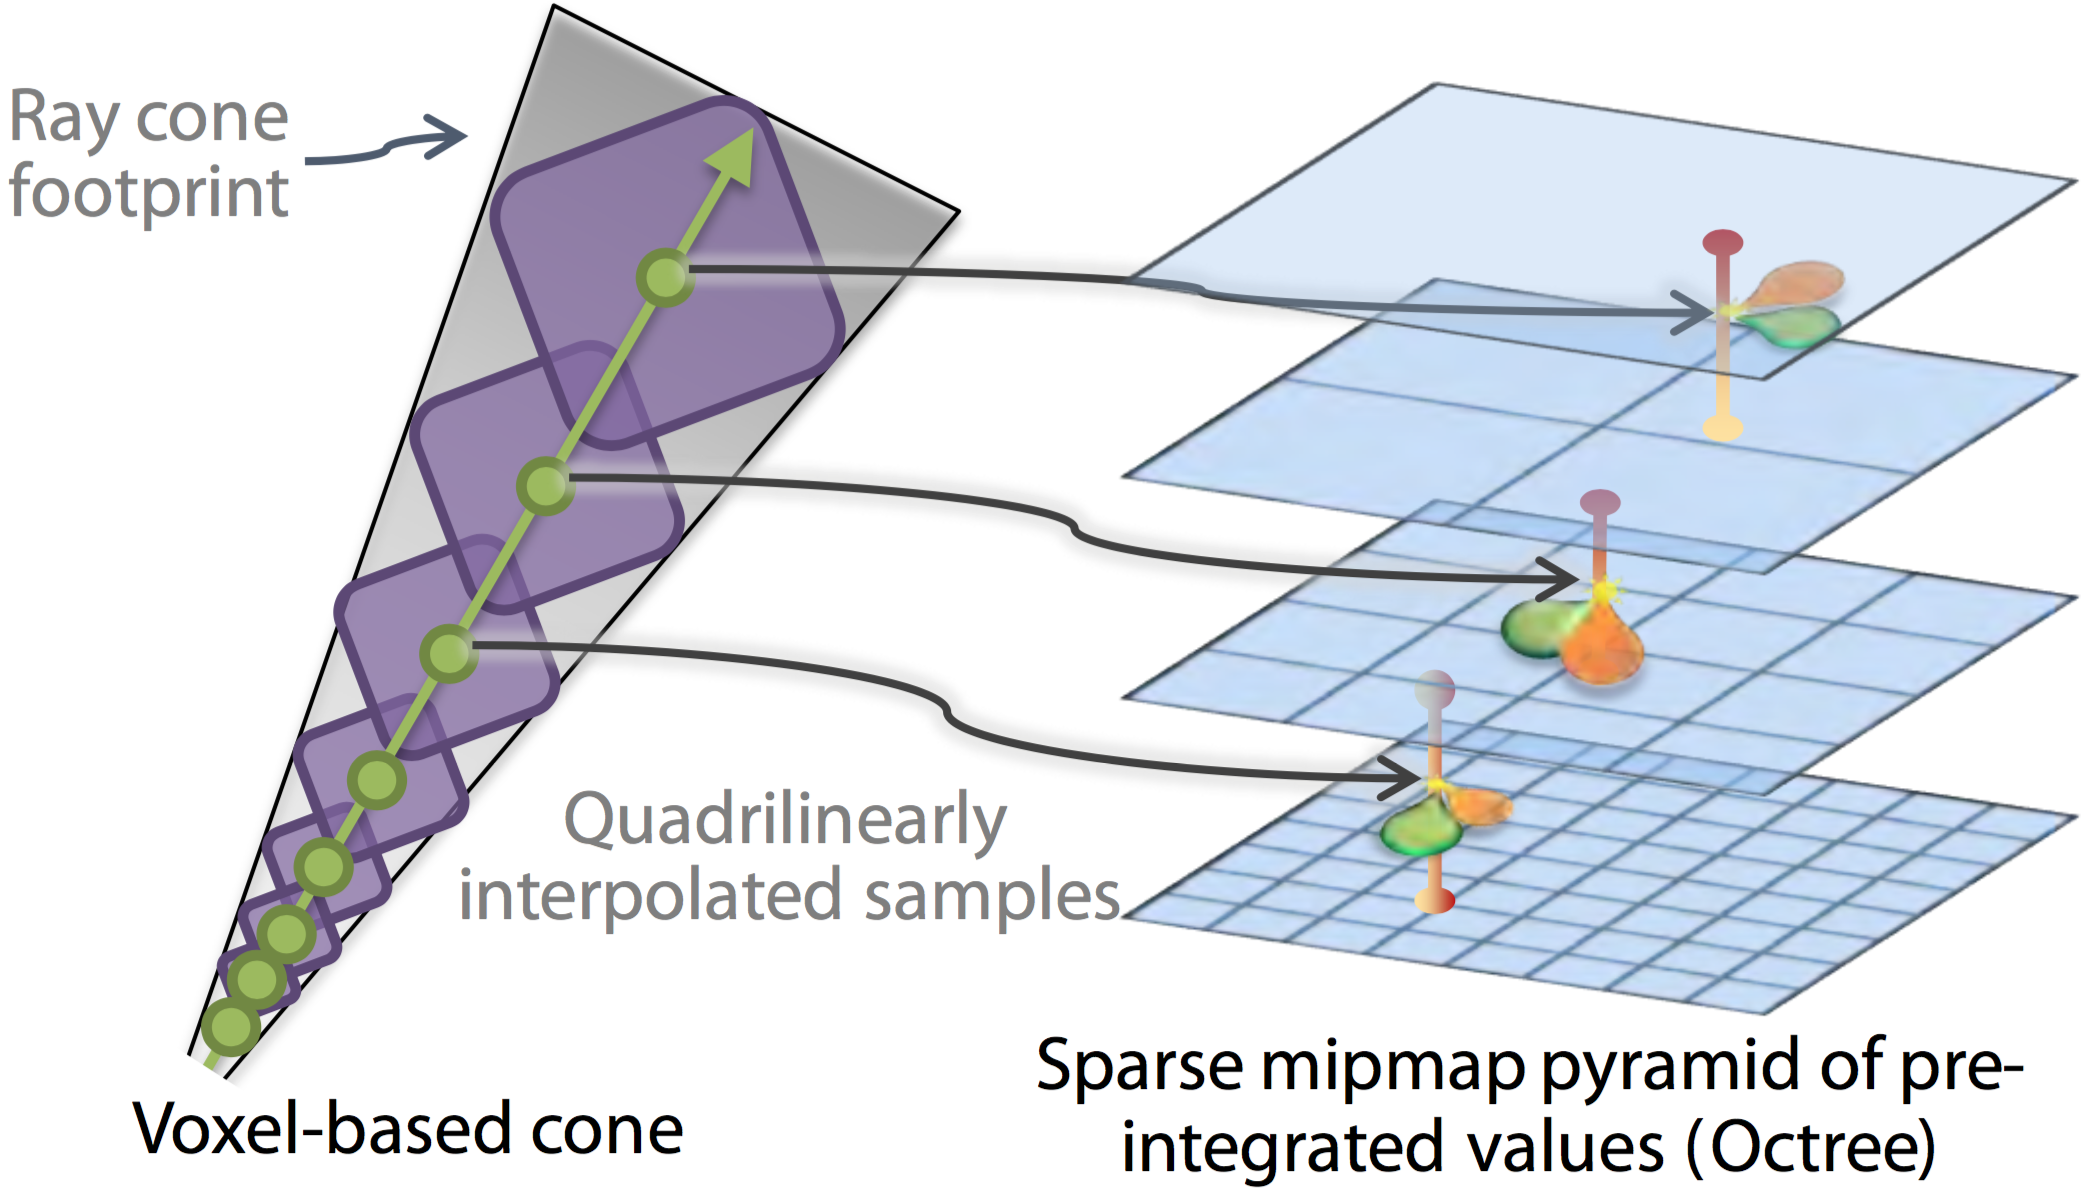
\includegraphics[width=0.65\textwidth]{figures/vct/vct-7-4}
	\caption{基于体素的圆锥 体追踪,它通过光线步进的 方式,多分辨率的体素结构 进行采样,这些体素包含预 过滤的光照和几何材质信 息,通过使用四线性插值, 这些体素内的多个光线的结 果可以被高效地近似(图片 来自\cite{a:Gigavoxels:Avoxelbasedrenderingpipelineforefficientexplorationoflargeanddetailedscenes})}
	\label{f:vct-cone-tracing}
\end{figure}

在圆锥体步进的过程中,我们使用传统的基于参与介质的光学模型来累积 各个采样的体素的光照值,其理论推导过程可以参见本章第\ref{sec:vct-pre-integration-based-cone-tracing}节的内容。我 们持续记录一个遮挡系数 $\alpha$,以及一个由各个体素累积的颜色值 $c$,这个颜色 值代表了整个圆锥体内的表面对圆锥体原点方向的反射光照。在每一次步进中, 我们得到每个体素对应的遮挡值 $\alpha_2$ 和光照贡献 $c_2$,然后使用传统体积渲染模 型从前向后地累积所有体素的光照贡献,即:

\begin{equation}
\begin{aligned}
	c:=&\alpha c+(1-\alpha)\alpha_2c_2\\
	\alpha=&\alpha+(1-\alpha)\alpha_2
\end{aligned}
\end{equation}

同时,为了保证更好的积分质量,由于步进中两个连续相邻的采样位置之 间的距离 $d^{'}$ 并不完全等于当前体素的尺寸 $d$,所以这里对遮挡值作出了适当的修正,即使用:$\alpha^{'}_s=1-(1-\alpha_s)^{\frac{d^{'}}{d}}$。



\subsection{环境遮挡}
为了说明这种近似的圆锥体追踪算法的运用,以及辅助更好地理解后面关 于间接光照的算法,我们这里首先讨论一个简单的情形,即对环境遮挡的估计, 因为环境遮挡只涉及可见性,所以暂时并不需要考虑复杂的光照计算。

环境遮挡(ambient occlusion,AO)\myindex{环境遮挡}{ambient occlusion}可以看做是一个可到达性的值,它是现 代实时渲染领域一个非常重要的概念,我们还会在下一章继续讨论环境遮挡的 不同估计方法。环境遮挡的概念源于环境光照,如前一章的内容可知,由于间 接光照的计算非常复杂,所以我们一些渲染算法尝试使用一个烘焙的环境贴图 来提供间接光照,使间接光照的计算转化为普通的对纹理的采样计算。这种方 法虽然高效,但是由于它忽略了物体表面上的位置点与光源之间的可见性,即 是假设所有表面点都没有被遮挡,因此整个渲染结果显得很“平面”,缺乏由于阴 影遮挡产生的立体感,所以环境遮挡的概念被提出,它用来估计一个表面位置 的可到达性,然后这个比例值被用于缩放来自环境贴图的光照,因此能够呈现 出物体表面的一些明暗细节,使场景更加立体。环境遮挡通常并不要求很精确 的值,它们大都通过一些近似的方法计算而出,例如它们通常忽略方向性,只 考虑整个半空间相对于该表面点的可到达性。

表面上某个点 $p$ 的环境遮挡 $A(p)$ 可以定义为在半空间 $\Omega$ 上关于可见性的 积分,即:

\begin{equation}
	A(p)=\cfrac{1}{\pi}\int_{\omega}V(p,\omega)\cos \omega{\rm d}\omega
\end{equation}

\noindent 其中,$V (p,\omega)$ 是一个可见性函数,如果源自位置 $p$ 且沿方向 $\omega$ 的光线与任 何物体相交,则其值为 0,否则为 1。

在实践中,通常对于室内的场景,由于没有无尽空旷的天空,其可见性往往被局限于一定的距离,因为最终所有可见性会被墙面遮挡,所以\cite{a:InteractiveIndirectIlluminationUsingVoxelConeTracing}提出对遮挡值 $\alpha$ 作用一个权重函数 $f(r)$,该权重函数(这里使用 $\cfrac{1}{1+\lambda r}$)随着距离而逐渐衰退,由此经过修改之后的遮挡值为:

\begin{equation}
	\alpha_f(p+r\omega):=f(r)\alpha (p+r\vec{\omega} )
\end{equation}

\noindent 为了有效地计算积分 A(p) 的值,这里将半空间划分为多个积分和的形式:

\begin{equation}
\begin{aligned}
	A(p)=&\cfrac{1}{N}\sum^{N}_{i=1}V_c(p,\Omega) \text{,其中}\\
	V_c(p,\Omega)=&\int_{\Omega}V_{p,\theta}\cos\theta{\rm d}\theta
\end{aligned}
\end{equation}

对于一种比较规则的划分,每个部分积分$V_c(p, \Omega_i)$ 的积分范围类似于一 个圆锥体。作为一个粗略的近似,我们可以将余弦函数部分从积分 $V_c$ 中分离 出来,这样积分就只包括可见性值,而这正是体素中存储的值,所以我们就可 以使用上述的基于体素的圆锥体追踪方法来计算环境遮挡,如图\ref{f:vct-14-1}所示。其可见性积分 $V(p,\omega)$ 仅仅需要累加体素中的可见性参数即可,将所有细分的圆锥体的可见性累加就得到了像素最终的环境遮挡值。

\begin{figure}
	\sidecaption
	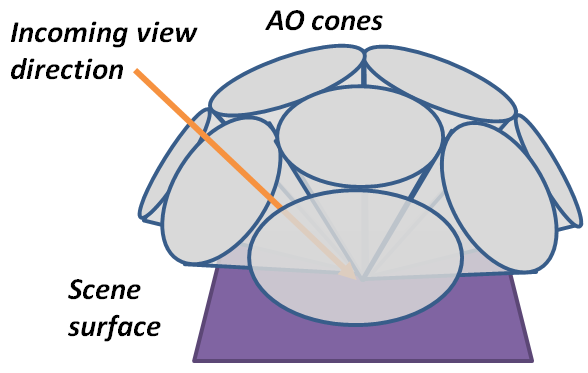
\includegraphics[width=0.5\textwidth]{figures/vct/vct-14-1}
	\caption{使用基于体素的 基元表述,环境遮挡可以被 划分为多个圆锥体的光束, 这些圆锥体的可见性可以直 接从体素中获得(图片 来自\cite{a:InteractiveIndirectIlluminationUsingVoxelConeTracing})}
	\label{f:vct-14-1}
\end{figure}

为了计算场景中表面的环境遮挡,只需要从当前视角执行一个光栅化渲染, 然后在每个像素着色器中执行上述的圆锥体追踪近似计算。为了进一步提高效 率,我们可以使用延迟着色以避免对被遮挡的体素执行上述的圆锥体追踪计算。



\subsection{间接光照}
间接光照的计算要比上述的环境遮挡要复杂得多,这也是我们要实现的主 要目标。为了更好地理解利用体素表述以及圆锥体追踪来计算间接光照,我们 重新来审视一下相关的理论基础。对于一个被采样的体素对其圆锥体原点方向 光照的贡献,综合式\ref{e:vct-reflection-equation-1}和式\ref{e:vct-voxel-distribution-1}可以得到如下的体素着色公式:

\begin{equation}\label{e:vct-voxel-shading}
	L({x},\omega_o)=\int_{S^{2}}L(x,\omega_i)\Biggl(\int_{S^{2}}\rho(\omega_i,\omega_o;\mathbf{n}){\rm d}\mathbf{n}\Biggl){\rm d}\omega_i
\end{equation}

对于上式右边最内部的积分,我们称它为一个“体素 BRDF 分布函数”,即 我们把一个体素视作为一个像素,该体素内所有表面细节的法线分布被封装在 了该体素 BRDF 分布函数中,然后我们将该体素 BRDF 分布函数与入射光照 的乘积进行积分,便可以按一般的反射公式计算体素的光照贡献。

对于这个体素 BRDF 分布函数,它涉及表面的真实(像素级别的)BRDF 分布函数与体素内表面法线分布函数乘积的积分,由于体素的法线分布函数已 经被封装为一个高斯分布,并且在构建体素数据结构的时候已经将其存储在体 素中,考虑表面的 BRDF 分布函数也为高斯分布的话,这个体素 BRDF 分布 函数的积分值就是两个高斯分布的卷积,我们在第\ref{sec:vct-local-shading}节已经介绍了相关的 方法计算这个卷积,这个卷积计算是在渲染的时候实时进行的,这样我们便可 以避免那些不会产生光照贡献的体素的局部着色计算。此外,需要注意的是,虽然我们假设这里表面的 BRDF 模型为冯氏模型,但是上述的逻辑并没有限制 BRDF 的形式,只是其它 BRDF 模型与法线分布函数(高斯分布)的卷积计 算(相比两个高斯分布之间的卷积计算)会稍微复杂,所以只要有比较高效的 卷积计算,理论上是可以对表面使用任意 BRDF 模型的。

一旦计算出了上述的体素 BRDF 分布函数,对于式\ref{e:vct-voxel-shading}表述的体素着色 公式,我们还需要知道该体素接受的入射光照能量 $L({x}, \omega_i)$,这也是渲染阶段主 要要做的事情,一旦得到每个体素的入射光照能量,便可以直接通过式式\ref{e:vct-voxel-shading}计 算出该体素的光照贡献。

为了得到体素的入射光照能量,本节的开头已经说明,我们使用两个步骤 来计算,如图\ref{f:vct-steps}所示。首先,我们在八叉树的叶节点上捕捉来自场景中所有 点光源的入射能量,然后我们对这些叶节点执行过滤,将这些入射能量分配到 八叉树的所有节点上。需要注意的是,由于我们存储的是体素的入射光照及其 方向信息,即入射光照的分布,因此这种方法能够处理光泽反射,如图\ref{f:vct-diffuse-vs-specular}(b)所示。如果体素的入射光照分布也表述为一个高斯分布,那么式\ref{e:vct-voxel-shading}外部的 积分又是两个高斯分布的卷积而已。

\begin{figure}
	\begin{subfigure}[b]{0.5\textwidth}
		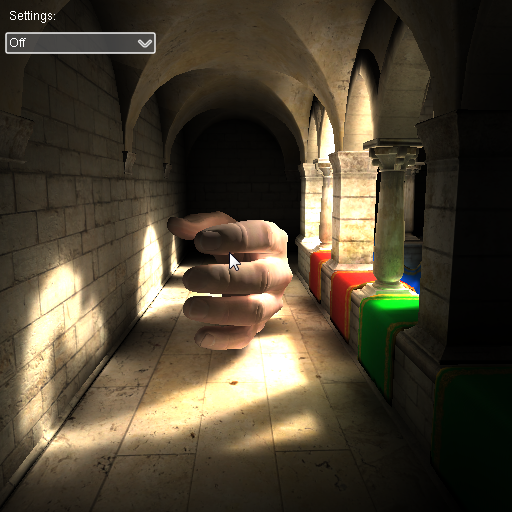
\includegraphics[width=\textwidth]{figures/vct/vct-14-2}
		\caption{漫反射}
	\end{subfigure}
	\begin{subfigure}[b]{0.5\textwidth}
		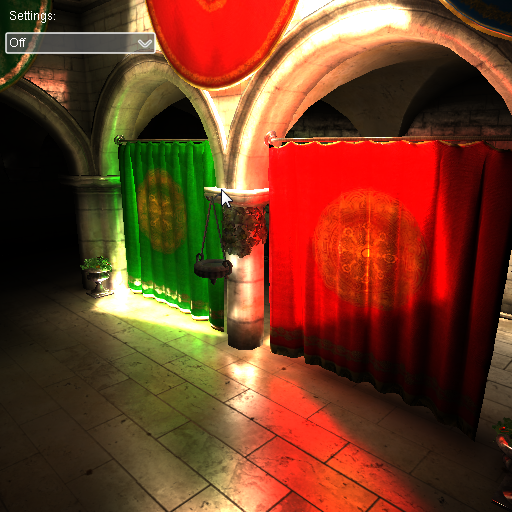
\includegraphics[width=\textwidth]{figures/vct/vct-14-3}
		\caption{光泽反射}
	\end{subfigure}
	\caption{基于体素的全局光照技术能够同时处理低频的漫反射光照(a),以及光泽反射(b)(图片来自\cite{a:InteractiveIndirectIlluminationUsingVoxelConeTracing})}
	\label{f:vct-diffuse-vs-specular}
\end{figure}

有了上述关于体素的入射光照分布,以及相关的着色模型,我们便可以对 表面执行圆锥体追踪来计算其间接光照。需要注意的是,本章介绍的方法只处 理两次反弹的间接光照,即光从光源发出,经过体素的一次反射,然后从摄像 机可见的表面反射至摄像机。\cite{a:TheTechnologyofTheTomorrowChildren} 中介绍了相关的方法来计算三次 反弹乃至多次反弹的间接光照。

不同于其它近似方法,如上一章介绍的那些基于球谐函数近似的方法,基 于体素的全局光照算法能够同时处理任意 BRDF 模型,严格地说,本章的内容 介绍的是一种框架模型,它并没有限制其中任何一个部分的频率,虽然我们主 要是针对冯氏模型进行讨论。

最后的渲染过程,即图\ref{f:vct-steps}中的第三步,跟前面介绍的环境遮挡的计算是 类似的,我们使用延迟渲染来剔除那些不可见的体素。在每个表面位置,我们使 用圆锥体追踪来计算来自所有光线步进过程中采样得到的体素的光照贡献值。



\subsubsection{捕捉直接光照信息}
现在来讨论怎样对体素存储入射光照信息。受反射阴影贴图(reflective shadow maps)\myindex{反射阴影贴图}{reflective shadow maps}的启发\cite{a:ReflectiveShadowMaps},我们将场景从光 源的视角按光栅化管线输出所有(对该光源)可见表面的世界坐标位置, 在其光栅化过程中,每个像素代表了一个光子,这些光子将从体素所在的位置 发生反射,其反射的光照将作为场景中其它(相对于摄像机位置及其视图可见 的)表面的间接光照。称这样的贴图为一个光源视图贴图(light-view map)\myindex{光源视图贴图}{light-view map}。

我们的目标,就是要将这些光子存储在八叉树节点当中。更准确地说,我们 需要存储的关于光子的信息包括两个方面,即光子的方向分布和光子的能量,这 个怎么理解呢?入射光能量不应该是一个关于辐射亮度的分布么,即在不同方 向上可能具有不同的辐射亮度,那样入射能量的分布函数就应该是一个四维的 函数,其中三维用于表述方向,而另外一维表示每个方向对应的辐射亮度值。这 样的分布函数是非常复杂的,并且它使得着色计算非常复杂,所以式\ref{e:vct-reflection-equation-1}其实隐式地包含了一个近似假设,为了方便说明,这里重新复制一下式\ref{e:vct-reflection-equation-1}, 即:

\begin{equation}
\begin{aligned}
	L({x},\omega_o)=&\cfrac{1}{N}\sum_{q\in {x}}\int_{S^{2}}L({x},\omega_i)\rho(\omega_i,\omega_o;\mathbf{n}(q)){\rm d}\omega_i\\
	=&\int_{S^{2}}L({x},\omega_i)\Biggl(\cfrac{1}{N}\sum_{q\in {x}}\rho(\omega_i,\omega_o;\mathbf{n}(1))\Biggl){\rm d}\omega_i
\end{aligned}
\end{equation}

这里其实假设一个体素内所有位置处的入射能量值是相同的,这样 $L({x}, \omega_i)$ 可以作为一个常数独立于后面的体素 BRDF 函数,否则就不可能 将积分后面的部分形成一个单独的新的积分,即体素 BRDF 分布函数。这种假 设其实是成立的,因为体素的尺寸相对于体素到光源的距离是非常远的,在其 对应的立体角内入射光照的能量变化可以忽略不计,并且即使光源很近,光子 的分辨率通常要远远大于体素的分辨率,所以这种假设仍然成立。基于这样的假设处理,入射光照分布就可以仅保留一个方向分布和一个常数的能量值,而 这个能量值(对于点光源)显然应该正比该光子面积所形成的立体角的大小,而 方向分布用于提供入射辐射亮度的方向,这个方向仍然可以使用一个高斯分布 来近似。

为了将光子从光源“洒向”体素,我们对上述的光源视图中的每个像素使用 一个像素着色器,因为光源视图贴图的分辨率通常高于最低层级的体素的分辨 率,所以每个光子可以完全直接洒向八叉树的其中一个叶节点。而且,这样的 光子始终会被落于八叉树的叶节点中,因为这些光子最终始终会落于物体表面 上,而不是在空白区域或者物体内部,而物体的表面位置始终会位于某个叶节 点表述的体素内。

此外需要注意的是,和八叉树结构的构建过程一样,由于每个光子都要自 上向下地访问八叉树,并且由于光子的分辨率高于叶节点的分辨率,多个光子 很可能同时访问一个相同的叶节点,所以这里仍然需要使用互斥锁。

上述的过程看似简单,但是由于体素块包含了冗余,即每个体素的值会被重复出现在其相邻的节点中,前面已经说明这种冗余是为利用 GPU 的硬件插值过滤特性,这种复制操作就可能导致 多个线程对节点访问的冲突,这将严重影响性能,所以需要一种高效的方法执行这种复制操作。





\subsubsection{向相邻块传递光照值}
在叶节点的体素被注入光照之后,为了实现上述的冗余,我们还需要把每个叶节点的光照复制到其相邻的叶节点体素纹理中。为了简化描述,这里我们假设八叉树的每个叶节点都是完全的,这样我们的算法只需要对每个叶节点发起一个复制操作的线程。

这里使用六个渲染通道,其中每个坐标轴$(x,y,z)$包含两个通道。例如在第一个$x-$轴的通道中,如图\ref{f:vct-light-transfer}左小图所示,每个线程会将当前体素的体积数据添加到其右边体素的相应数据位,这意味着每个线程会添加三个数据项,例如原始左边的三项数据为$(3,4,0)$,右边原始的三项数据为$(4,2,1)$,则添加后右边体素的数据为$(7,6,1)$;接下来的通道则会将右边(被加和之后)的数据项传输回左边,这通过直接复制到左边并覆盖原来的数据项即可,在这一步之后,沿着$x-$轴上的所有数据都变得连贯(coherent),例如相邻的数据都为$(7,6,1)$。最后我们对其他$y-$和$z-$轴执行相似的过程。

\begin{figure}
	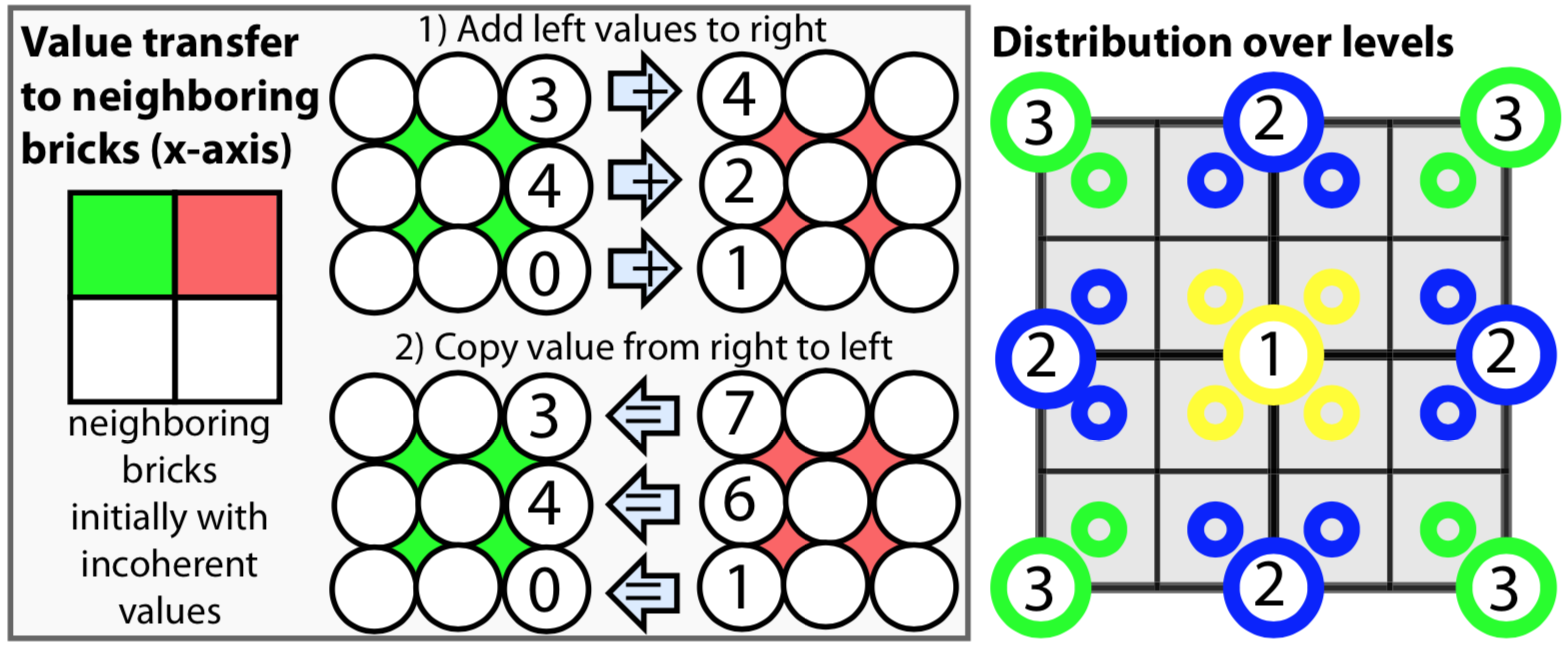
\includegraphics[width=\textwidth]{figures/vct/light-transfer}
	\caption{左图:当光子被“洒向”各个叶节点之后,由于相邻体素之间存在复制的体素,所以需要沿着坐标轴向相邻位置进行复制传输; 右图:为了从高分辨率向更低分辨率的体素进行过滤,这里使用三个通道进行计算,每个低分辨率的纹素对来自高分辨率的体素的三个通道的计算结果进行加和(图片来自\cite{a:InteractiveIndirectIlluminationUsingVoxelConeTracing})}
	\label{f:vct-light-transfer}
\end{figure}

上述的方法是非常高效的,因为我们存储了相邻体素的指针,这使得我们可以快速的读取到相邻体素的数据;同时上述的过程避免了线程访问的冲突,其间甚至不涉及任何原子操作。



\subsubsection{入射能量的过滤}
最后我们需要对八叉树叶节点的体素执行过滤,以生成一个多分辨率的体素结构。一种比较简单的思路是直接对每个低分辨率的体素使用一个线程,然后每个线程分别从高分辨率的体素中读取数据进行加权过滤。尽管这个方法比较简单,但是它有一个缺点:因为我们的体素结构存在冗余,所以相同的体素会被读取多次,这可能多达八次重复相同的计算,并且每个线程的计算量是不平衡的。

\cite{a:InteractiveIndirectIlluminationUsingVoxelConeTracing}使用三个独立的通道来实现体素的过滤,并且这三个通道拥有相似的计算成本,如图\ref{f:vct-light-transfer}右小图所示。其主要的思路是每次只计算最终过滤结果的一部分,然后使用上一节讨论的块之间的数据传输来完善最终的结果。

第一个通道只计算节点中间的位置,它使用高分辨率结构中相关的27个体素进行计算,如图中的黄色小圆所示;第二个通道计算位于节点面上的中间位置,它只计算最终过滤结果的一半,所以只涉及到18个体素,如图中的蓝色小圆所示;第三个通道则计算节点拐角处的位置,它仍然只计算最终过滤计算的一部分,其只涉及到一个体素,如图中的绿色小圆所示。

当三个通道完成之后,上述的计算结果实际上已经形成了一个低分辨率的体素结构,它的结果类似于上一节当中对叶节点进行光子撒播后的结果,即八叉树的每个节点可能只包含一部分,通过在相邻节点之间进行数据传输,就构成了一个完整的结果。因此这里仍然可以对上述的结果执行上一节的数据传输来形成最终完整的过滤结果。

